% arara: pdflatex
% arara: bibtex
% arara: makeglossaries
% arara: pdflatex
% arara: pdflatex
\documentclass[ngerman,a4paper,12pt,pdftex]{report}
\usepackage{dhpaper}
\usepackage{lipsum}
\usepackage[utf8]{inputenc} 
\usepackage[T1]{fontenc}
\usepackage[upright]{fourier} 
%\usepackage[usenames,dvipsnames]{xcolor}
\usepackage{tkz-kiviat,numprint,fullpage} 
\usepackage{pgfplots}
\usepackage{float}
\pgfplotsset{compat=1.16}


\usetikzlibrary{arrows}
\thispagestyle{empty}


\def\SymbReg{\textsuperscript{\textregistered}}


\hypersetup{
	pdfborder = {0 0 0}
}

%\includeonly{
%    intro,
%    foundations,
%    body,
%    conclusion,    
%    qualitativeStudy,
%    beobachtungen,
%    quantitativeStudy,
%    glossary
%}

\makeglossaries
\newacronym{rtfm}{RTFM}{Read The Fucking Manual}
\newacronym{gnu}{GNU}{GNU is Not Unix}
\newacronym{wtf}{WTF}{What The Fuck}
\newacronym{fubar}{FUBAR}{Fucked Up Beyond All Repair}
\newacronym{guc}{GUC}{German University of Cairo}
\newacronym{mbti}{MBTI}{Myers-Briggs-Typenindikator}

\newglossaryentry{report}
{
    name=Bericht,
    description={Eine strukturierte Darstellung von Inhalten aus Datenbeständen}
}

\newglossaryentry{programminglanguage}
{
    name=Programmiersprache,
    description={Eine formale Sprache zur Formulierung von Datenstrukturen und Algorithmen}
}

\newglossaryentry{dummy}
{
    name=Dummy,
    description={Ein Platzhalter, der (vorerst) nicht zum Funktionieren eines Programms benötigt wird}
}

\newglossaryentry{Lego}
{
	name=Lego,
	description={Ein dänischer Klemmbausteinhersteller, welcher mit seinen Sets Lego WeDo und Lego Mindstorms\SymbReg programmierbare Roboter zum Bauen und Spielen herstellt}
}

\newglossaryentry{Konvergenz}
{
	name={konvergentes Denken},
	description={Konvergentes Denken, convergent thinking, nach J. P. Guilford beschreibt das gleichgerichtete Denken, dessen Merkmale zusammenführend, analysierend, in Richtung einer einzigen, genauen Lösung zielend sind \cite{convergentThinking}}
}

\newglossaryentry{Emergenz}
{
	name=Emergenz,
	description={Unter Emergenz versteht man in der Psychologie die spontane Herausbildung von neuen Eigenschaften oder Strukturen auf der Makroebene von Systemen infolge des Zusammenspiels seiner Elemente \cite{emergentThinking}}
}

\newglossaryentry{Divergenz}
{
	name={divergentes Denken},
	description= {Divergentes Denken, divergent thinking, bedeutet, sich offen, unsystematisch und experimentierfreudig mit einem Thema oder Problem zu beschäftigen, wobei das divergente Denken  das Gegenstück zum konvergenten Denken darstellt \cite{divergentThinking}}
}



\bibliography{dhpaper}

\begin{document}

% project details
\projecttitle{Technologiegestütztes Lernen am Beispiel von LEGO}
\projectauthor{Janick Kaltenmark \& Timo Steidinger}
\projecttype{Studienarbeit}
\studentid{5771742 \& 1877259}


% timeline
\deadline{06.05.2021}
\duration{26 Wochen}

% school information
\schoolname{DHBW Karlsruhe}
\schoollogo{icon_dhbw}
\schooladvisor{Prof. Dr. Kay Berkling}

% degree information
\degreetype{Bacherlor of Science}
\subject{Informationstechnik}
\courseid{TINF19B3}

\maketitlepage

\makestatement

%\makenda

% table of contents, listings
\pagenumbering{gobble}
\tableofcontents

\clearpage
\pagenumbering{roman}
\setcounter{page}{1}
% list of figures
\listoffigures
\addcontentsline{toc}{chapter}{Abbildungsverzeichnis}

% list of tables
\listoftables
\addcontentsline{toc}{chapter}{Tabellenverzeichnis}

% list of abbreviations, glossary of terms
\printglossary[title={Abkürzungsverzeichnis},type=\acronymtype]


% list of code listings
%\lstlistoflistings
%\addcontentsline{toc}{chapter}{Codelistingverzeichnis}

% actual body of the report
\begin{onehalfspace}
    \clearpage
    \pagenumbering{arabic}
    % main body of the report, separated by chapters
    \chapter{Intro}


\section{Motivation}

In dem Artikel \citetitle{stephanidis_seven_2019} werden die großen Herausforderungen aufgeführt, welche zukünftig an das Gebiet des \acrshort{hci} (acrlong{hci}) gestellt werden, also an die wechselseitige Interaktion des Menschen mit Maschinen.\\  Immer schneller schreitet der technologische Fortschritt voran. Dies führt nicht nur dazu, dass die Erwachsenen sich auf die neue Technologie stetig neu einstellen müssen, sondern auch dazu, dass die Kinder von heute vor immer komplexere Probleme gestellt werden, die diese Technologie mit sich bringt. Und so führen \citeauthor{stephanidis_seven_2019} den Bereich \textit{Lernen und Kreativität} als eine dieser großen Herausforderungen an. Besonders die Informatik ist von diesem Problem betroffen. Schüler entwickeln hier oft nur oberflächliche Kenntnisse, anstelle von Strategien zum Lösen von Problemen wie \citeauthor{kazimoglu_serious_2012} in \citetitle{kazimoglu_serious_2012} beschreibt. \cite{kazimoglu_serious_2012}.\\
Doch die Technologie stellt nicht nur Herausforderungen, sondern bietet auch Chancen. So lassen sich Technologien in den Lernprozess integrieren, dieser lässt sich sogar durch die Technologie leiten. Dies ist nichts Neues. Bereits im Jahr 2000 gab es mit der \textit{Addy}-Reihe zahlreiche Lernspiele für verschiedene Schulfächer und Altersstufen \cite{addy}. Auch jüngere Altersgruppen wurden bereits \citeyear{wyeth_tangible_2002} von \citeauthor{wyeth_tangible_2002} an die Informatik herangeführt, indem Bausteine so mit Elektronik versehen wurden, dass je nach dem, wie die Steine aufeinander gesteckt werden, unterschiedliche Aktionen ausgeführen \cite{wyeth_tangible_2002}. \\
Doch auch in der jüngeren Vergangenheit gibt es neue Technologien, um Kinder und Jugendliches an verschiedene Lernthemen heranzuführen, wie beispielsweise ein Programm zum Üben der Rechtschreibung an Grundschulen \cite{berkling_learning_2020}.\\
Diesen Trend hat auch \gls{Lego} erkannt, die mit \gls{Lego}-Education seit dem Jahr 1999 eine eigene Produktsparte nur für den Zweck, an Schulen eingesetzt zu werden, anbieten. Die Effektivität dieser Produkte wird von zahlreichen wissenschaftlichen Arbeiten erörtert und belegt \cite{perez_new_2015, karatrantou_algorithm_2008, jun_design_2016, cuellar_design_2014, klassner_lego_2003}\\
Ein weiterer Aspekt des Lernens mithilfe von Technologie ist die Möglichkeit, dass sich die Lernumgebung an den Lernenden anpasst. Beliebt ist hierbei der \acrlong{mbti}. \citeauthor{yel_adaptive_2018} haben beispielsweise ein Modell erstellt, bei dem sich die genannten Lernabschnitte(\textit{Einführung}, \textit{Inhalt}, \textit{Übertragung} und \textit{Übung}), nach dem \acrshort{mbti} an den Lernenden anpassen \cite{yel_adaptive_2018}.\\
In dieser Arbeit soll qualitativ der Fortschritt einer Gruppe von Kindern während der Vorbereitung auf den Wettbewerb \acrlong{fll} dokumentiert und untersucht werden. Dabei soll insbesondere auf die Entwicklung der Kinder in den verschiedenen Kategorien (Teamwork, Computational Thinking) sowie Zusammenhänge zwischen diesen Entwicklungen und dem \acrshort{mbti} der Kinder geachtet werden.



\section{Beschreibung des Projektablaufes}
Im Rahmen des Projektes wurden im wöchentlichen Abstand regelmäßig Kurse mit Lego WeDo 2.0. durchgeführt. Durch die Autoren der Studienarbeit wurde die Mitarbeit der Kinder mithilfe von im Vorhinein erstellten Beobachtungsbögen beobachtet. Diese legen einen Fokus unter anderem auf die Motivation, Kreativität sowie auf die Teamarbeit und das algorithmische Denken. Die Kinder führten dazu im Vorhinein einen Test durch, welcher sie in unterschiedliche Persönlichkeitskategorien unterteilt \cite{knowAndLove}. Ebenfalls wurde zu Beginn der Test von \citeauthor{zapata_bctt_2021} in \citetitle{zapata_bctt_2021} durchgeführt, um das algorithmische Denken der Kinder zu untersuchen.
Um die Ergebnisse nicht mit den Kindern in Verbindung zu bringen, bekam jedes Kind ein Pseudonym. Die Pseudonyme wurden zum Teil von den Eltern der Kinder bei der Anmeldung festgelegt, die restlichen Namen wurden durch die Autoren aufgefüllt.\\
Gleichzeitig fand eine Zusammenarbeit der Autoren mit einer Parallelveranstaltung an der \acrlong{guc}(\acrshort{guc}) statt, die bei ihrer Vorbereitung auf die \acrshort{fll} ebenfalls den Fortschritt der Kinder in den Beobachtungsbögen festhielten.


\section{Daten}
Die Rohdaten, die für die Studienarbeit verwendet wurden, werden nach Abschluss der Arbeit auf GitHub hochgeladen, so dass diese verfügbar sind für eventuelle weitere Arbeiten, die auf dieser basieren. Der Link dazu ist folgender: \url{https://github.com/janick3110/technologyenhancedLearningData}
    \chapter{Grundlagen}

\section{Die \acrlong{fll}}
Bei der \acrlong{fll}(\acrshort{fll}) handelt es sich um Wettbewerbe, die von einer Kooperation von \gls{Lego} und \gls{First} organisiert werden. Das Ziel dieser Wettbewerbe ist es Kinder und Jugendliche für eine Laufbahn im \gls{MINT}-Bereich zu motivieren. In Zentraleuropa wird die \acrshort{fll} von dem Verein HANDS on TECHNOLOGY e.V. betrieben.\\
Mittlerweile besteht die \acrshort{fll} aus zwei Wettbewerben. Die \acrlong{fll} Explore für Kinder im Grundschulalter (6-10 Jahre) und die \acrlong{fll} Challenge für Kinder und Jugendliche der weiterführenden Schulen. Diese beiden Wettbewerbe haben ein gemeinsames Saisonthema, welches in dieser Saison (2021/22) das Thema \textit{Transport} war.\\

\subsection{Der Ablauf der \acrshort{fll} Explore} \label{preparation}
In der Vorbereitungszeit wird den Kindern von der \acrshort{fll} Explore ein IngenieurInnen Notizbuch und ein Motivationsset mit \gls{Lego}-Teilen zugeschickt. In diesem Notizbuch gibt es für jedes Treffen eine Seite mit Fragen und Aufgaben zum Saisonthema. Gelegentlich wird als Aufgabe auch ein Projekt aus der Projektbibliothek \ref{Projektbibliothek} gestellt. Die Aufgaben in dem Notizbuch drehen sich jedoch generell eher um das kreative Bauen, wie \textit{entwirf ein Transportmittel für das Wasser}, als um bewegliche und programmierbare Modelle. Somit nimmt das Programmieren in der Vorbereitung auf die \acrshort{fll} eine etwas untergeordnete Rolle ein.\\
Zuletzt wird von den Teams gefordert, ein Teammodell zu entwerfen, welches sie am Wettbewerbstag den Richtern vorführen und präsentieren. Hierzu soll ebenfalls ein Teamposter erstellt werden.


\section{Das Baukastensystem LEGO WeDo2.0} \label{Wedo}
Zur Durchführung der Kurse wurde der Baukasten LEGO WeDo 2.0 verwendet. Dessen Eigenschaften und Konzepte sollen hier erläutert werden.
\subsection{Das Konzept des Baukastens}
Die LEGO WeDo Produktreihe zielt darauf ab, Kindern spielerisch Inhalte der Naturwissenschaft und Technik, sowie grundlegende Programmierkonzepte zu vermitteln. Hierfür werd von LEGO Handbücher für Lehrer, Leitfäden sowie die Software mit der die Elektronischen Bauteile programmiert werden können zur Verfügung gestellt. Somit richten sich die Baukästen speziell an Schulen und andere Bildungseinrichtungen. Zu den Baukästen gibt es jeweils ein äquivalentes Produkt für zuhause, welches jedoch weniger technische Bauteile (Balken, Achsen, Zahnräder) sondern mehr bunte und dekorative Bauteile enthält.\\ 
Der Vorgänger des WeDo 2.0 Baukastens musste noch über ein USB Kabel direkt mit dem Computer verbunden sein. Des weiteren, enthielt dieser lediglich einen Motor, dessen Drehrichtung und Geschwindigkeit vom Computer aus eingestellt werden konnte. Aufgrund der benötigten USB Verbindung war es nicht möglich die Modelle von Tablet-Computern oder Smartphones zu steuern.  \\
Dahingegen verfügt der verwendete WeDo 2.0 Baukasten über zwei Sensoren und einen Motor. Des weiteren wird keine USB Verbindung mehr benötigt, sondern der Programmierbare Baustein über Bluetooth angesteuert. Durch die App kann neben einem normalen Computer auch über einen Tablet-Computer oder ein Smartphone programmiert werden.

\begin{figure}[htbp!]
	\centering
	\fbox{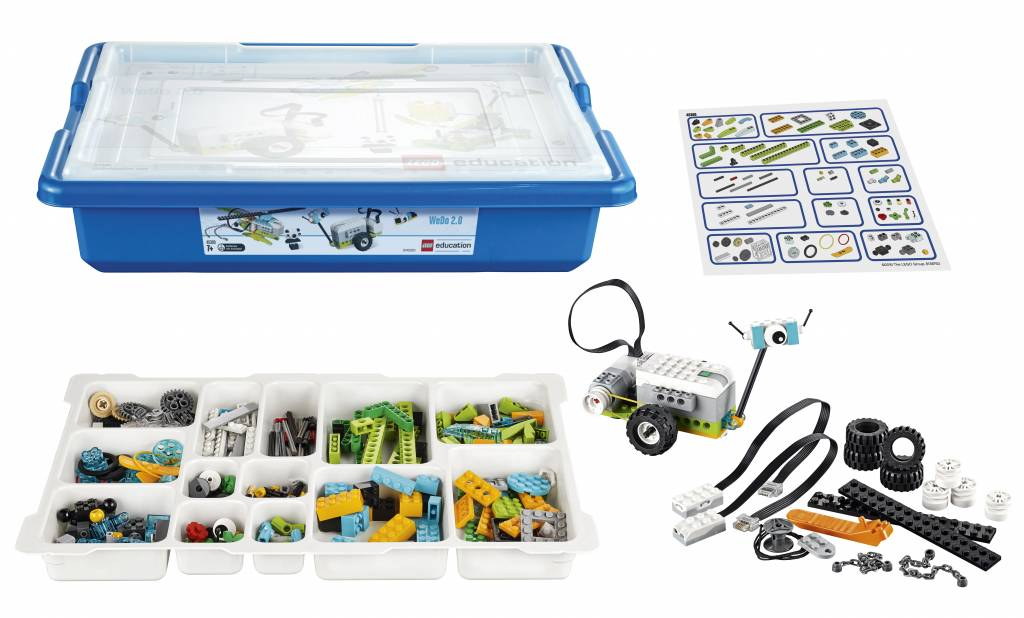
\includegraphics[width=0.4\textheight,angle=0]{img/lego-education-wedo-20}}
	\caption[Der WeDo 2.0 Baukasten]{Der WeDo 2.0 Baukasten} % \cite{knowAndLove}
	\label{img:lego-education-wedo-20}
\end{figure} 

\subsection{Inhalt}

\subsection{Die Projektbibliothek}\label{Projektbibliothek}
Das Programm zu dem WeDo 2.0 Baukasten bietet eine Projektbibliothek (Abb. \ref{img:projects}). Die Projekte innerhalb dieser haben alle einen ähnlichen Aufbau. Das Thema der Projekte ist aus dem \gls{MINT}-Bereich. Zu diesem werden den Kindern zunächst einige Fragen gestellt. Anschließend können sich die Kinder ein kleines Video zu dem Thema ansehen, welches die Kinder auf das Thema einstimmen soll. Beispielsweise ist in dem Video zum Thema \textit{Standfestigkeit} eine Erdkugel mit Kontinentalplatten, ein Seismograph, Aufnahmen von Erdbeben und verschiedene Gebäude, wie Hochhäuser und Pyramiden, zu sehen.\\
Anschließend dürfen die Kinder das Modell zu dem Thema bauen. Das in \ref{img:subject} gezeigte Modell zum Thema \textit{Standfestigkeit} stellt einen vereinfachten Erdbebensimulator dar, mit drei Modellgebäuden.\\
\begin{figure}[htbp!]
	\centering
	\fbox{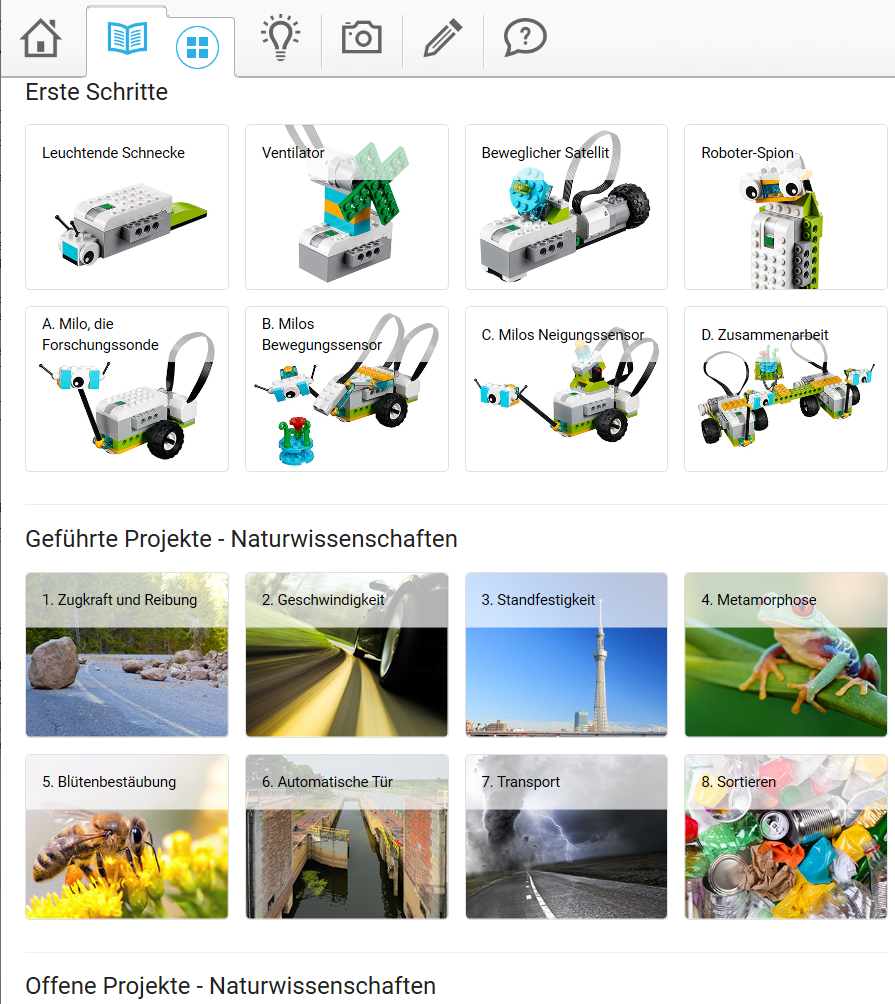
\includegraphics[width=0.4\textheight,angle=0]{img/Projects.png}}
	\caption[Die Programmbibliothek]{Die Programmbibliothek}
	\label{img:projects}
\end{figure} 

\begin{figure}[htbp!]
	\centering
	\fbox{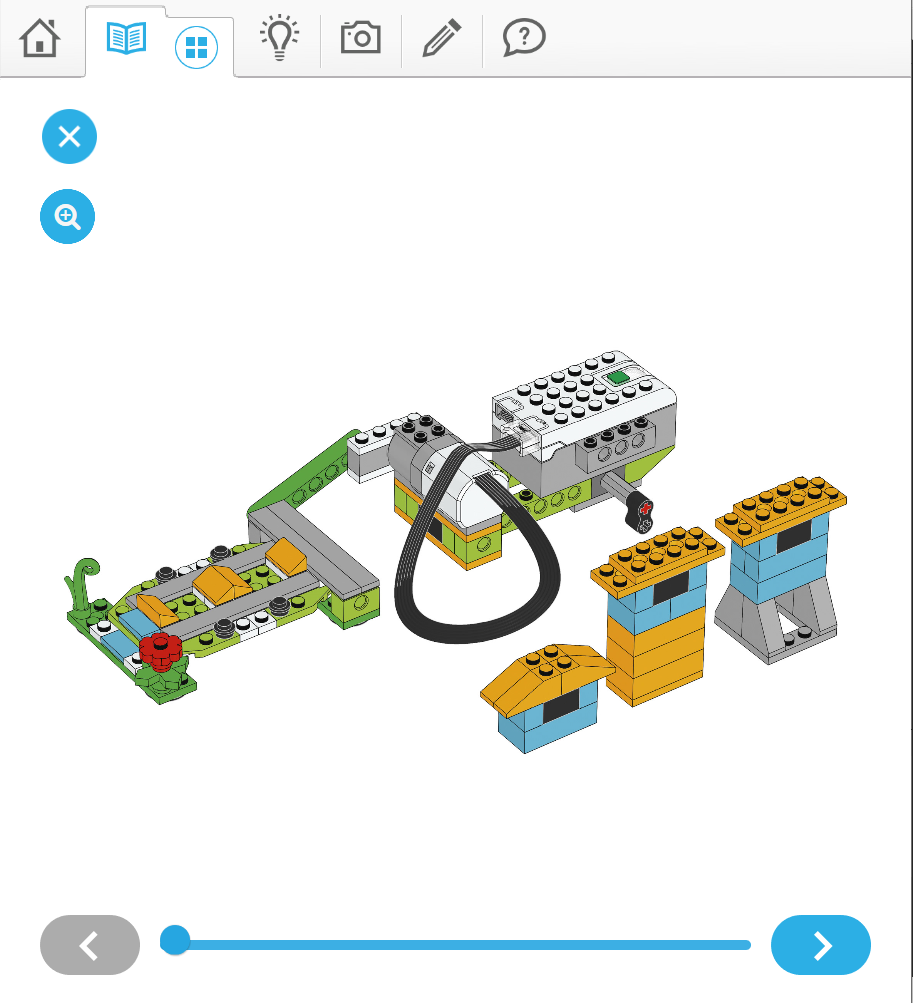
\includegraphics[width=0.4\textheight,angle=0]{img/Model.png}}
	\caption[Das Modell zum Thema Standfestigkeit]{Das Modell zum Thema \textit{Standfestigkeit}}
	\label{img:subject}
\end{figure} 

Nach dem Bau wird das Modell von den Kindern programmiert. Hierzu steht den Kindern eine Programmvorlage zur Verfügung, welche sie nachbauen können. Diese ist für das Projekt \textit{Standfestigkeit} in \ref{img:programtemplate} zu sehen. Dabei wird Motorgeschwindigkeit, welche die Erdbebenstärke simuliert, bei jedem Durchlauf um eins erhöht und der Motor für zwei Sekunden gedreht.\\
Daraufhin sollen die Kinder das Modell mit dem Programm ausprobieren.\\
Zum Abschluss kann den Kindern noch eine Kompetitive Aufgabe gegeben werden, bei der sie das Modell und Programm verbessern sollen. Bei dem Thema Standfestigkeit ist das die Aufgabe, ein Gebäudemodell zu entwerfen, welches der größten Erdbebenstärke standhält und gleichzeitig am höchsten ist.

\begin{figure}[htbp!]
	\centering
	\fbox{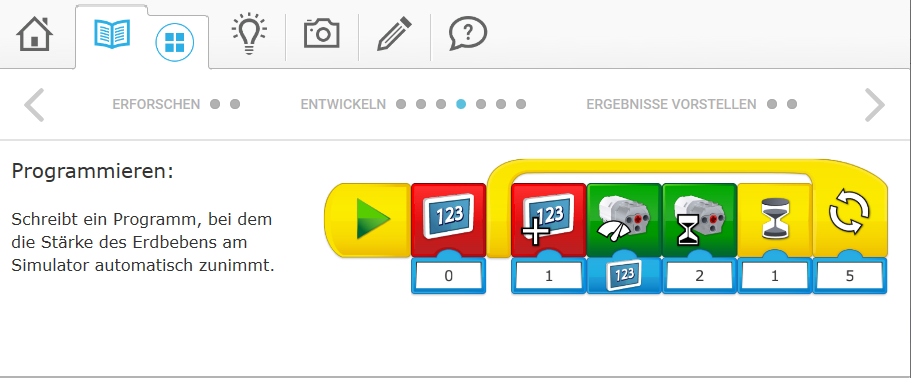
\includegraphics[width=0.4\textheight,angle=0]{img/programtemplate.png}}
	\caption[Die Programmvorlage]{Die Programmvorlage bei dem Thema \textit{Standfestigkeit}}
	\label{img:programtemplate}
\end{figure} 

\subsection{Programmieren mit WeDo 2.0}\label{WedoSoftware}
Um für Kinder leichter greifbar zu sein, wurde zum programmieren der Modelle eine Oberfläche gewählt, bei der einzelne Programmblöcke hintereinander gezogen werden. Die Abfolge der Blöcke ergibt damit das fertige Programm. Nach ihrer jeweiligen Funktion lassen sich die Programmblöcke in Kategorien einteilen. Eine Einteilung ist von LEGO durch die Farbgebung der Programmblöcke bereits gegeben. \\
Einige Blöcke benötigen einen zusätzlichen Wert, der ihnen übergeben werden muss. Diese sind mit einer halbkreisförmigen Öffnung an der Unterseite versehen. Die Blöcke, welche diese Werte liefern, hingegen sind mit einer halbkreisförmigen Wölbung versehen. 

\subsubsection{Die Aktionsblöcke}
\begin{figure}[htbp!]
	\centering
	\fbox{\includegraphics[width=0.4\textheight,angle=0]{img/Aktionsblöcke.png}}
	\caption[Die Aktionsblöcke]{Die Aktionsblöcke} % \cite{knowAndLove}
	\label{img:Aktionsblöcke}
\end{figure}

Mit den Aktionsblöcken Abb. \ref{img:Aktionsblöcke} können Motoraktionen und die Farbe der Statusleuchte gesteuert werden. Für den Motor kann einerseits die Richtung in welche sich der Motor dreht, die Geschwindigkeit und die Dauer der Motordrehung gesteuert werden.

\subsubsection{Die Arithmetik- und Medienblöcke}
\begin{figure}[htbp!]
	\centering
	\fbox{\includegraphics[width=0.4\textheight,angle=0]{img/LogikProgrammblöcke.png}}
	\caption[Die Arithmetik und Medienblöcke]{Die Arithmetik und Medienblöcke} % \cite{knowAndLove}
	\label{img:ArithmetikUndMedienblöcke}
\end{figure}
Mangels einer besseren Bezeichnung für diese Kategorie werden deren Blöcke hier als  Arithmetik- und Medienblöcke bezeichnet (Abb. \ref{img:ArithmetikUndMedienblöcke}). Es können einerseits Geräusche und Töne abgespielt werden. In der Bibliothek stehen 28 unterschiedliche Tonaufnahmen zur Verfügung. Ebenfalls können Bilder auf dem Bildschirm angezeigt werden. Die Tonaufnahmen und Bilder aus der Bibliothek passen jeweils Thematisch zu den Projekten aus der Projektbibliothek \ref{Projektbibliothek}. Die Bibliothek kann jedoch durch eigene Tonaufnahmen und Bilder ergänzt werden. Die Bilder und Tonaufnahmen werden von dem Gerät aus abgespielt, über welches das Modell programmiert wird, da der programmierbare Legostein, der die Befehle von dem Master-Gerät entgegennimmt, weder über ein Display, noch über Lautsprecher verfügt.\\
Mit den beiden Arithmetikblöcken können einfache Berechnungen durchgeführt werden. Es kann lediglich ein einziger Wert als Variable existieren. Dieser wird auf dem Bildschirm als große Zahl angezeigt. Das erlaubt die Beobachtung des Wertes, während der Programmausführung. Zur Verfügung stehen die Operationen: \textit{Plus}, \textit{Minus}, \textit{Mal} und \textit{Geteilt durch}.\\
Mit dem letzten Block dieser Kategorie (ganz rechts) kann das Bild und die Variable die angezeigt wird vergrößert oder verkleinert werden.

\subsubsection{Die Programmablaufblöcke}
\begin{figure}[htbp!]
	\centering
	\fbox{\includegraphics[width=0.4\textheight,angle=0]{img/Programmablaufblöcke.png}}
	\caption[Die Programmablaufblöcke]{Die Programmablaufblöcke} % \cite{knowAndLove}
	\label{img:Programmablaufblöcke}
\end{figure}
In Abb. \ref{img:Programmablaufblöcke} sind die Blöcke zu sehen, welche den Programmablauf steuern. Bei den drei linken Blöcken handelt es sich um die verschiedenen Startblöcke.\\
Der mit dem grünen Pfeil erlaubt den Start eines dahinterliegenden Programmteils mittels eines einfachen Knopfdrucks. Mit dem zweiten Block kann der Programmteil durch einen Buchstaben der Tastatur gestartet werden. Der Buchstabe mit dem das Programm gestartet wird, kann für jeden einzelnen dieser Blöcke geändert werden, sodass ein leichtes Auswählen verschiedener Programmteile ermöglicht wird.\\
Der dritte Startblock mit dem Briefumschlag, der in einen Briefkasten geworfen wird, als Symbolbild kann ein Programm durch ein Signal aus einem anderen Programmteil gestartet werden. Das Signal wird von dem Block rechts daneben gesendet, mit dem Briefumschlag als Symbolbild. Diesem wird ein Wert übergeben und anschließend wird der Startblock gestartet, der den gleichen Wert hat. \\
Der Block mit der Sanduhr dient dazu, eine bestimmte Zeit zu Warten. Er kann jedoch auch dafür verwendet werden, auf einen Sensorzustand zu warten. Ein kleines Beispiel zu dem Programmstart mit dem Postkasten-Block und dem Warten-Block ist in Abb. \ref{img:Beispiel_01} zu sehen. Dabei wird nach Starten des Programms durch den grünen Pfeil, zunächst der obere Programmteil gestartet, welcher den Motor nach rechts drehen lässt und nach einer Sekunde der untere Programmteil, der den Motor nach links drehen lässt. 



\begin{figure}[htbp!]
	\centering
	\fbox{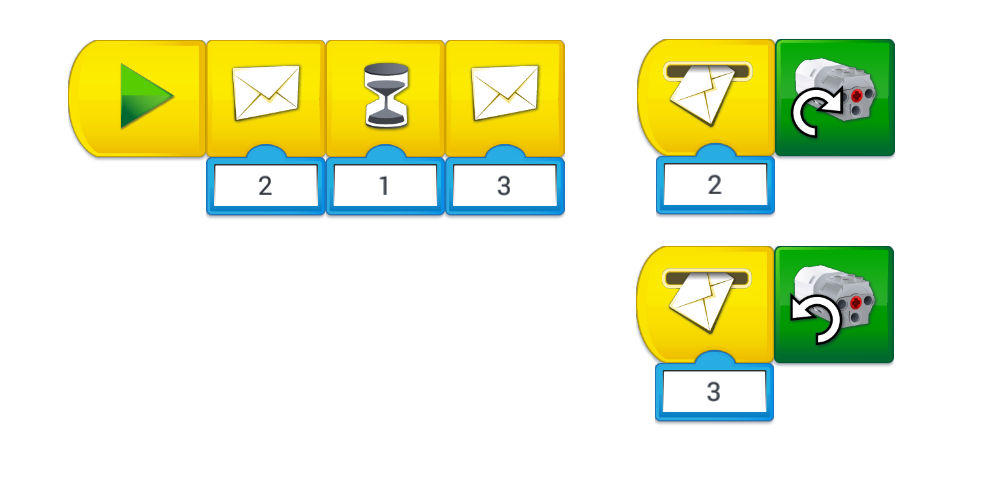
\includegraphics[width=0.4\textheight,angle=0]{img/Example_01.png}}
	\caption[Beispielprogramm zum Start aus anderem Programmteil]{Beispielprogramm zum Start aus anderem Programmteil} % \cite{knowAndLove}
	\label{img:Beispiel_01}
\end{figure}

\subsubsection{Wertblöcke}

Die Blöcke, welche zusätzliche Werte zur Konfiguration benötigen können über die Wertblöcke andere Werte zugewiesen bekommen. Diese Art Blöcke wird in die halbkreisförmige Öffnung des Blockes gehängt, dem ein neuer Wert zugewiesen werden soll. \\
Zur Verfügung stehen Zahlenwerte, Zeichenketten, die Variable vom Bildschirm und ein zufälliger Zahlenwert zwischen 0 und 10.

\begin{figure}[htbp!]
	\centering
	\fbox{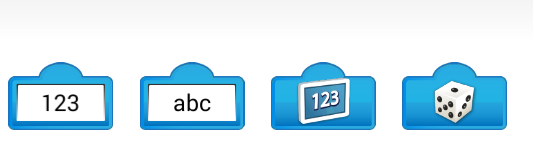
\includegraphics[width=0.4\textheight,angle=0]{img/Werte.png}}
	\caption[Werte]{Werte}
	\label{img:Werte}
\end{figure}


\subsubsection{Sensorwertblöcke}

Diese Blöcke werden verwendet, um Blöcken einem Sensorwert zuzuweisen. Die Blöcke können Werte zwischen 0 und 10 annehmen und bilden somit ihre Messwerte auf dieser Skala ab.\\
Der Kippsensor weist jeder Kipprichtung einen Ganzzahlwert zu. Damit kann eine Hebelsteuerung realisiert werden. \\
Der Distanzsensor misst grob eine Distanz zu Hindernissen. Damit kann Beispielsweise ein Automodell vor einer Wand zum stehen gebracht werden.\\
Der Lautstärkesensor misst grob die Umgebungslautstärke. Damit kann ein Programm durch klatschen gestartet werden.

\begin{figure}[htbp!]
	\centering
	\fbox{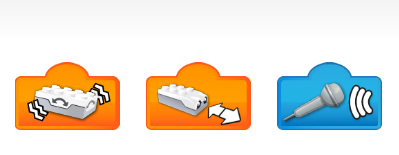
\includegraphics[width=0.4\textheight,angle=0]{img/Sensoren.png}}
	\caption[Sensorwerte]{Sensorwerte} % \cite{knowAndLove}
	\label{img:Sensorwerte}
\end{figure}


\section{Die Kurse}






\section{Myers-Briggs-Typenindikator\textsuperscript{\textregistered}} 
\subsection{Typen nach Jung}
Der Psychoanalytiker Carl Gustav Jung definierte im 20. Jahrhundert insgesamt acht verschiedene Typen. Diese Typen sind unterteilt in zwei Kategorien mit je vier Typen. Die beiden Kategorien, die Jung definierte, sind die Kategorie \glqq Extrovertiert"' und \glqq Introvertiert"'. In beiden Kategorien sind jeweils die vier Typen Fühlend, Denkend, Intuitiv und Empfindend. \cite{jung_1921}\\

In den folgenden Abschnitten werden mithilfe des Werks \citetitle{jung_2014} Jungs Kategorien sowie die Typen kurz zusammengefasst.
\subsubsection{Extrovertiert}
Nach \citeauthor{jung_2014} sind Menschen, welche in Jungs Kategorie der Extravertierung
fallen, sehr lebhafte Menschen, die den Kontakt zu Anderen lieben. Wenn extravertierte Menschen sich an eine Gruppe anpassen müssen, fällt ihnen das sehr einfach. Menschen, die als extravertiert bezeichnet werden, werden häufig als störend bezeichnet. Ihrer eigenen Innenwelt wird von diesen Menschen nur wenig Achtung geschenkt, was sie als eher oberflächliche Menschen wirken lässt. Wenn es um Tätigkeiten geht, übernehmen extravertierte Menschen Rollen, welche organisatorischer, kreativer oder repräsentativer Art sind. 

\noindent
\cite{jung_2014}

\subsubsection{Introvertiert}

Introvertierte Menschen sind das Gegenteil der Extrovertierten. Sie scheuen den Kontakt mit der Außenwelt und sind dadurch viel mehr auf ihr Inneres fokussiert. Diese Menschen zeigen nach dem Autor \citeauthor{jung_2014} des Werks \citetitle{jung_2014} häufig scheue und verschlossene Charakterzüge, seltener auch etwas weltfremde Züge. Dieser Typus von Menschen neigt nach dem Autor auch häufig zu Rechthaberei und Eigensinn, woraus Konflikte resultieren. Im Vergleich zu den eher praktischen Aufgaben, die extravertierte Menschen lieben, bevorzugen introvertierte Menschen eher die theoretischen Aufgaben.

\noindent
\cite{jung_2014}

\subsubsection{Fühlend}
Offenheit, Toleranz und Teamfähigkeit sind Eigenschaften, die nach Hans Jung und C. G. Jung dem extravertierten fühlenden Typus zugesprochen werden. Als charakterliche Züge werden diese Menschen als loyal und treu beschrieben. Da sich der extravertierte Typus weniger auf seine Innenwelt, sondern eher auf die Außenwelt fokussiert, beschränken sich auch die Gefühle des extravertierten Fühltypus nicht nur auf seine Innenwelt.\\
Sollte der Mensch sich mit seinen Gefühlen weniger auf die Außen-, sondern auf die Innenwelt beschränkt, handelt es sich um einen introvertierten Fühltypus. Die Urteilsbildung eines solchen Menschens werden von seinen eigenen persönlichen Werten geleitet. 

\noindent
\cite{jung_2014}
\subsubsection{Denkend}
\citeauthor{jung_2014} fasst den extravertierten Denktypus nach \citeauthor{jung_1921} als eine Person, welche sich analytisch mit seiner Welt auseinandersetzt und Bewertungen und Beurteilungen auf eine sachliche Weise durchgeführt werden. Das Treffen von Entscheidungen ist keine Hürde für extravertierte Menschen des Denktypus. Personen dieses Typs übernimmt wie bereits erwähnt gerne Tätigkeiten organisatorischer Art, da es in dessen Natur liegt zu versuchen, seine Umwelt zu organisieren.\\
Personen, welche dem introvertierten 



Der introvertierte Denktypus hingegen lässt sich nur mit Tatsachen überzeugen. 
Er denkt und handelt logisch, objektiv, kritisch und unpersönlich. Er versucht nicht 
seine Umwelt zu ändern oder ihr seine Ideen aufzudrängen. Negativ für einen solchen Typus ist, dass seine Gedankengänge für andere Personen schwer verständlich 
sind und diese ihn missverstehen können.
\subsubsection{Intuitiv}
Extravertiert: 
Intuition, als eine Art Ahnung oder Wahrnehmung auf unbewusste Weise, äußert sich 
bei dem extravertierten Typus in der Art, dass er über Ideenreichtum verfügt und 
Eingebungen mit hoher Zielstrebigkeit verfolgt, um zu prüfen, ob sie realisierbar sind 
oder nicht. Er verfügt über die Gabe andere Personen von seinen Ideen zu überzeugen, 
beziehungsweise regelrecht mitzureißen. Leider liegt ihm nichts an der Umsetzung. 
Sein Interesse flaut ab, wenn er sein Ziel erreicht hat und andere mit der Umsetzung 
betraut sind. 
Introvertiert: 
Beim introvertierten Typus richtet sich die Intuition auf das Erkennen von Potenzialen und Möglichkeiten, die sich aus unbewussten Inhalten ableiten. Der introvertierte 
Typus mag Herausforderungen, wenn diese Inspiration für seine Ideen und Visionen 
bieten. Ähnlich wie bei dem extravertierten Typus verliert er das Interesse, wenn das 
Projekt konkrete Formen annimmt und die Lösung bevorsteht.
\subsubsection{Empfindend}
Extravertiert: 
Empfindungen entstehen durch Sinnesreize, wie Geruch, Geschmack, Gehör, Tastsinn 
sowie Bewegung und Gleichgewicht. Der extravertierte Typ stützt sich auf seine 
Sinne, wobei Einzelheiten und Tatsachen Beachtung geschenkt wird. Die Einstellung seiner Umwelt gegenüber ist eher als sachlich und realistisch zu beschreiben. Er akzeptiert Tatsachen, kann aber nicht Veränderungen und neue Ideen akzeptieren, weil 
er sie nicht mit seinen Sinnen erfassen kann. 
Introvertiert: 
Der introvertierte Typ hingegen beschäftigt sich intensiv und sensitiv mit den Empfindungen in seinem Seelenleben, wobei er nach außen hin eher durch Neutralität auffällt. Er wird nie auf äußerliche Empfindungen und Eindrücke reagieren, sondern sich 
Zeit für innerliches Überlegen und Überdenken nehmen. Von daher kann man von 
ihm keine impulsiven oder spontanen Gefühlsausbrüche erwarten.




\section{Persönlichkeitscharaktere}

Der folgende Abschnitt geht genauer auf den Test für den Persönlichkeitstypus der einzelnen Kinder ein.

Der Test, den die Kinder durchgeführt haben, ordnet jedem Teilnehmer eine Tier zu. Jedes dieser Tiere steht für einen Typus nach dem \acrlong{mbti} (\acrshort{mbti}). Der \acrshort{mbti} besteht aus 16 verschiedenen Persönlichkeitstypen (vgl. Abbildung \ref{img:mbti}), bei denen jede der Typ die Überlagerung aus vier verschiedenen Attributen ist. Wie in der Abbildung dargestellt, gibt es damit 16 verschiedene Anordnungen der Zeichen E, F, I, J, N, P, S und T, wobei jedes Zeichen für ein bestimmtes Attribut steht. Insgesamt werden aus diesen Zeichen vier Paare gebildet: EI, SN, TF und JP. In einer Abkürzung nach Myer-Briggs kann jeweils nur ein Buchstabe eines Paares vorkommen, woraus die 16 Typen in Abbildung \ref{img:mbti} resultieren.
\begin{figure}[htbp!]
	\centering
	\fbox{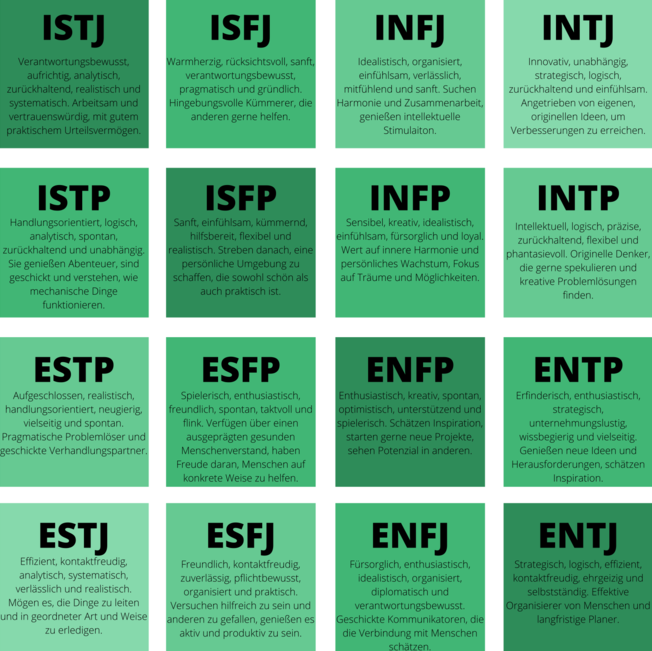
\includegraphics[width=0.35\textheight,angle=0]{img/Myers-Briggs-Typenindikator}}
	\caption[Myers-Briggs-Typenindikator]{Die 16 Persönlichkeitstypen nach Myers-Briggs}
	\label{img:mbti}
\end{figure}

Jeder einzelne Typ hat nach Myers-Briggs Auswirkungen auf Personen. \cite{myers_myers_2002} 
\begin{figure}[htbp!]
	\centering
	\fbox{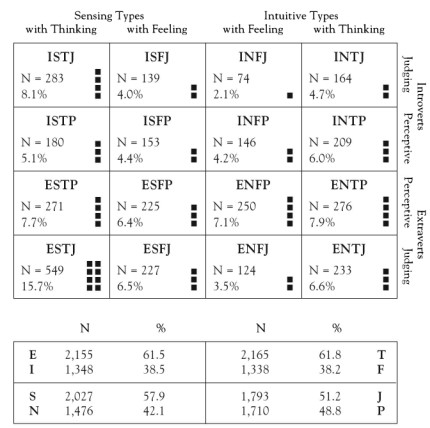
\includegraphics[width=0.35\textheight,angle=0]{img/distribution}}
	\caption[Verteilung der Myers-Briggs-Typen]{Verteilung der Myers-Briggs-Typen \cite{myers_myers_2002}}
	\label{img:mbti_distribution}
\end{figure}

\subsection{Studienrelevante Persönlichkeitscharaktere}
\subsubsection{Border Collie - ESTJ / ENTJ}
\begin{figure}[htbp!]
	\centering
	\fbox{
\includegraphics[width=0.2\textheight,angle=0]{img/Border_Collie}}
	\caption[Border Collie]{Border Collie}
	\label{img:Border_Collie}
\end{figure}
„Collie“ ist das schottisch-gälische Wort für „nützlich“. Sie sind logisch, entschlossen, kompetent und organisiert und bevorzugen eine Umgebung, in der sie ihre Intelligenz einsetzen, andere führen und aktiv gehalten werden können. Diese Kinder sind am glücklichsten, wenn sie die Möglichkeit haben, die Verantwortung zu übernehmen und sich zu messen. Sie genießen Herausforderungen, Debatten und die Interaktion mit einer Vielzahl von Menschen. Das Leben ist ein großer Wettbewerb, und sie sind entschlossen zu gewinnen.

\subsubsection{Elefant - ESFJ / ENFJ}
\begin{figure}[htbp!]
	\centering
	\fbox{
\includegraphics[width=0.2\textheight,angle=0]{img/Elephant}}
	\caption[Elefant]{Elefant \cite{knowAndLove}}
	\label{img:Elefant}
\end{figure}
Freundlich, aufgeschlossen und organisiert. Sie sind am glücklichsten, wenn sie anderen helfen, gesellschaftliche Veranstaltungen planen oder an Aktivitäten teilnehmen, an denen Menschen beteiligt sind – ALLE Menschen. Diese Kiddos bevorzugen ein harmonisches und kooperatives Umfeld mit viel Lob und Zuneigung. Im Leben dreht sich alles um echte Beziehungen und die Verbindung zu Menschen. 

Friendly, outgoing and organized. They're happiest when helping others, planning social events or participating in activities that involve people - ALL of the people. These kiddos prefer a harmonious and cooperative environment with lots of praise and affection. Life is all about genuine relationships and connecting with people.	\\
\subsubsection{Erdmännchen - INFP / ISFP}
\begin{figure}[htbp!]
	\centering
	\fbox{
\includegraphics[width=0.2\textheight,angle=0]{img/Meerkat}}
	\caption[Erdmännchen]{Erdmännchen \cite{knowAndLove}}
	\label{img:Elephant}
\end{figure}
Moralisch, sanft und sensibel mit einer kreativen und doch komplexen inneren Welt. Sie sind am glücklichsten in einer ruhigen, kooperativen und unterstützenden Umgebung, in der sie sinnvollen Dingen nachgehen können. Diese Kinder brauchen viel eingeplante Zeit allein, um ihre natürlichen Bauchgefühle zu verarbeiten und die Welt zu analysieren. Sie sind tief im Einklang mit den Gefühlen und Bedürfnissen anderer und neigen dazu, eine Friedensstifterrolle einzunehmen. Im Leben geht es darum zu verstehen, wie Menschen ticken. 

Moralistic, gentle and sensitive with a creative yet complex inner world. They're happiest in calm, cooperative and supportive environments where they can pursue meaningful matters. These kiddos need plenty of scheduled alone time to process their natural gut feelings and analyze the world. They are deeply in tune with others' feelings and needs and tend to take on a peacemaker role. Life is about understanding what makes people tick. \\	
\subsubsection{Panda - INFJ / INTJ}
\begin{figure}[htbp!]
	\centering
	\fbox{
\includegraphics[width=0.2\textheight,angle=0]{img/Panda}}
	\caption[Panda]{Panda \cite{knowAndLove}}
	\label{img:Panda}
\end{figure}
Intensiv privat, kreativ und ideenorientiert. Sie sind am glücklichsten, wenn ihre Bemühungen und einzigartigen Ideen anderen helfen, zu wachsen und zu lernen. Sie schätzen Autonomie und sind vertrauenswürdige, einzigartige, fähige und aufschlussreiche Personen. Diese Kinder bevorzugen eine ruhige Umgebung, in der sie in ihrer inneren Welt denken, verarbeiten und erschaffen können. Den Sinn hinter den Dingen zu verstehen, ist ihr Lebensziel. 

	Intensely private, creative and idea-oriented. They're happiest when their efforts and unique ideas help others to grow and learn. They appreciate autonomy and being trustworthy, unique, capable and insightful individuals. These kiddos prefer a calm environment where they can think, process and create in their inner world. Understanding the meaning behind things is their goal in life. \\
\subsection{Restliche Tiere}
Im folgenden wird zur Einordnung der bereits genannten Tiere in das gesamte Spektrum der Persönlichkeitstypen mit den Tieren, welchem keinem Kind in der Studie zugeordnet wurde, dargestellt.



\section{Computational Thinking} \label{sec:ct}
Um das informatische Denken der Kinder messen zu können, wurde mit den Kindern der Computational Thinking Test durchgeführt. Da die Kinder noch sehr jung sind, wurde deshalb die spezielle Variante für Jüngere, der sogenannte Beginners Computational Thinking Test, von den Kindern absolviert. Nach den Autoren des \acrshort{bctt}, \citeauthor{bcct}, ist die Fähigkeit des Computational Thinkings, eine kognitive Fähigkeit, welche für eine erfolgreiche Anpassung an die Zukunft wichtig ist, eine Kernfähigkeit. Dadurch, dass die Welt immer mehr den Schwerpunkt auf Technologie und Programmierungen legt, ist diese Fähigkeit des Computational Thinkings eine sehr kritische. Die Autoren des \acrshort{bctt} halten es für wichtig, dass Schüler und Schülerinnen in der Lage sein sollten, kritisch zu denken und komplexere Probleme lösen zu könne.\\
Die vier Kernelemente des Computational Thinkings sind Abstraktion, Dekomposition, Algorithmen und das Debugging.\\
\cite{bcct} 
\subsection{Beginners Computational Thinking Test}
Der \acrlong{bctt}, kurz \acrshort{bctt}, ist eine Weiterentwicklung des Computational Thinking Tests für Jüngere. Gemeinsam mit Experten wurde eine erste Version erstellt, welche mithilfe von Pilottests und Experten in eine zweite Variante verbessert wurde. Diese wurde anschließend an verschiedenen Schulen in Spanien durchgeführt.\\

Der \acrshort{bctt} ist in mehrere Segmente aufgeteilt. Insgesamt sind es drei große Kerngebiete, die wiederum in sechs verschiedene Aufgabengebiete aufgeteilt wurden, die der Test überprüft. Das erste Segment \glqq Sequences"' überprüft, ob die Kinder in der Lage sind, Sequenzen zu folgen. Dies ist das erste Kerngebiet des \acrshort{bctt}. Der zweite Abschnitt überprüft einfache Schleifen, der dritte Abschnitt überprüft verschachtelte Schleifen. Die beiden genannten Abschnitte bilden damit die Überprüfung für Schleifen. Das letzte Kerngebiet sind die sogenannten Conditionals. Dieses Kerngebiet wird von den drei Gebieten If-Then, If-Then-Else und While gebildet. Dort wird überprüft, ob die Kinder in der Lage sind, Anweisungen, welche an Bedingungen geknüpft sind, korrekt auszuführen.\\

Die Gebiete sind nicht gleich groß. Die Größe der Aufgabengebiete ist in der untenstehenden Tabelle dargestellt. Der größte Bereich wird vom Kerngebiet Schleifen gebildet, gefolgt von den Conditionals. Das kleinste Kerngebiet sind die einfachen Sequenzen.

\begin{table}[H]
	\centering
	\begin{tabular}{|l|l|}
		\hline
		Bezeichnung              & Anzahl Fragen \\ \hline
		Sequenzen                & 6             \\ \hline
		einfache Schleifen       & 5             \\ \hline
		verschachtelte Schleifen & 7             \\ \hline
		If-Then                  & 2             \\ \hline
		If-Then-Else             & 2             \\ \hline
		While                    & 3             \\ \hline
	\end{tabular}
	\caption{Anzahl Fragen pro Aufgabengebiet}
	\label{tab:distQuestions}
\end{table}

In Abbildung \ref{img:bcttQuestion} ist beispielhaft eine Frage eines Aufgabengebiets, hier das Gebiet der While-Conditionals, dargestellt. Eine Frage besteht immer aus einer Grafik und vier dazugehörigen Antworten, von denen nur eine richtig ist. Bei den Antwortmöglichkeiten sind die jeweiligen Anweisungen dargestellt, welche zur Lösung führen sollen. Die Aufgaben, bei denen neben Pfeilen auch andere Symbole verwendet werden, wie in der untenstehenden Abbildung dargestellt, beinhalten noch eine zusätzliche Anweisung für die Person, die den Test bearbeitet. 

\begin{figure}[H]
	\centering
	\fbox{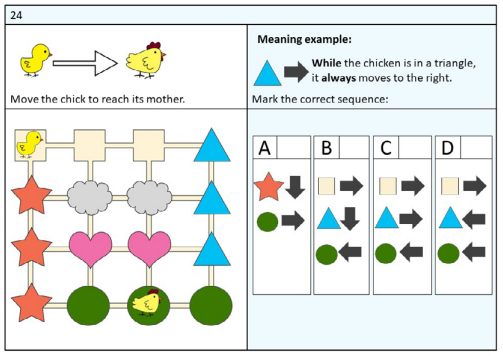
\includegraphics[width=0.4\textheight,angle=0]{img/bcttQuestion}}
	\caption[Beispielhafte Frage des \acrshort{bctt}]{Beispielhafte Frage des \acrshort{bctt}\cite{bcct}}
	\label{img:bcttQuestion}
\end{figure}

Die zweite Version des Tests wurde so abgeändert, dass auch Farbenblinde diesen Test durchführen können, weshalb die Felder in Abbildung \ref{img:bcttQuestion} mit Symbolen versehen wurden statt wie ursprünglich nur farbig dargestellt. Dies hat den Vorteil, dass zusätzlich der Test nicht zwingend in Farbe gedruckt werden muss, sondern auch in schwarz-weiß gut lösbar ist. \cite{bcct}

Der Test wurde wie bereits erwähnt an mehreren Schulen in Spanien angewendet. Insgesamt wurde eine Stichprobe von 299 Schüler und Schülerinnen an drei verschiedenen Schulen durchgeführt. Die Schüler und Schülerinnen waren in verschiedenen Klassenstufen, so dass der Test die Klassen 1,2,4,5 und 6 abdeckte. Für die Studienarbeit sind die Daten der Schüler und Schülerinnen relevant, welche die zweite Variante des \acrshort{bctt} durchführten. Die Ergebnisse nach \citeauthor{bcct} sind in der untenstehenden Tabelle dargestellt. Für die Studienarbeit nicht relevante Daten wurden aus Gründen der Übersichtlichkeit nicht übertragen.

\begin{table}[H]
	\centering
	\begin{tabular}{|l|l|l|l|}
		\hline
		\rowcolor[HTML]{C0C0C0} 
		Klassenstufe & N  & durchschnittliches Ergebnis & Standardabweichung \\ \hline
		2            & 18 & 14.278                      & 2.445              \\ \hline
		4            & 28 & 21.286                      & 1.922              \\ \hline
		6            & 25 & 21.280                      & 3.542              \\ \hline
	\end{tabular}
	\caption[Statistiken des \acrshort{bctt}]{Statistiken des \acrshort{bctt} nach \citeauthor{bcct}}
	\label{tab:statisticsBCTT}
\end{table}


\section{Torrance Tests}{
	\label{sec:torrance_tests}
	\begin{figure}[H]
		\centering
		\fbox{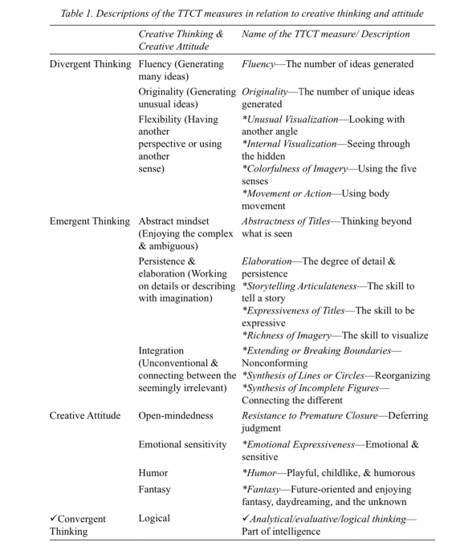
\includegraphics[width=0.4\textheight,angle=0]{img/ttct}}
		\caption[Relation von TTCT-Maßnahmen]{Relation von TCTT-Maßnahmen gegenüber kreativem Denken und kreativer Haltung \cite{Kim2016}}
		\label{img:ttct}
	\end{figure}
}

    \chapter{Qualitative Studie}
	Im folgenden Abschnitt werden die Durchführung der Studie sowie die genaueren Ergebnisse und Beobachtungen aufgeführt, welche im Verlauf der Studie gewonnen werden konnten. Es werden jedoch nur die reinen Beobachtungen und Ergebnisse hier aufgeführt, die Fazite werden erst in einem späteren Kapitel behandelt.
\section{Teilnehmerübersicht}
	Es folgt ein kurzer Überblick über die acht Teilnehmer der Studie.\\
	Insgesamt nahmen acht Kinder an den Terminen teil. Die Kinder waren zum Zeitpunkt dieser Arbeit noch in der Grundschule, jedoch nicht alle in der gleichen Klassenstufe. Die Kinder kannten sich zum Teil bereits untereinander bevor die Studie begann.Es wurde folgende Anzahl von Persönlichkeitstypen im Vorfeld abgegeben: drei Elefanten, zwei Border Collie, zwei Erdmännchen und ein Panda. Die Zuordnung der Tiere lautete wie folgt: Heinz, Lulu und Moritz als Elefanten, Jonas und Mario als Border Collies, Henriette und Benny als Erdmännchen und Sara als Panda.\\
	
	\begin{table}[H]
		\centering
		\begin{tabular}{|
				>{\columncolor[HTML]{C0C0C0}}c |c|c|c|}
			\hline
			\textbf{Typ} & \cellcolor[HTML]{C0C0C0}\textbf{Anzahl n} & \cellcolor[HTML]{C0C0C0}\textbf{Verteilung in \%} & \cellcolor[HTML]{C0C0C0}\textbf{Differenz in \%} \\ \hline
			ENTJ//INFJ   & 2                                         & 25                                                & +2,7                                             \\ \hline
			ENFJ//ESFJ   & 3                                         & 37,5                                              & -27,5                                            \\ \hline
			ISFP//INFP   & 2                                         & 25                                                & -16,4                                            \\ \hline
			INTJ//INFJ   & 1                                         & 12,5                                              & -5.7                                             \\ \hline
		\end{tabular}
		\begin{tabular}{|
				>{\columncolor[HTML]{C0C0C0}}c |c|c|c|}
			\hline
			\textbf{Typ} & \cellcolor[HTML]{C0C0C0}\textbf{Anzahl n} & \cellcolor[HTML]{C0C0C0}\textbf{Verteilung in \%} & \cellcolor[HTML]{C0C0C0}\textbf{Differenz in \%} \\ \hline
				E            & 5                                         & 62,5                                             & +1,0                                                 \\ \hline
				I            & 3                                         & 37,5                                             & -1,0                                                 \\ \hline
				T            & 3                                         & 33,3                                             & -28,5                                                \\ \hline
				F            & 6                                         & 66,6                                             & +28,5                                                \\ \hline
				S            & 5                                         & 62,5                                             & +4,6                                                 \\ \hline
				N            & 3                                         & 37,5                                             & -4,6                                                 \\ \hline
				J            & 6                                         & 75,0                                             & +23,8                                                \\ \hline
				P            & 2                                         & 25,0                                             & -23,8                                                \\ \hline
			\end{tabular}
		\caption[Verteilung der Typen unter den Teilnehmern]{Verteilung der Typen unter den Teilnehmern und Abweichung von Myers und Myers \cite[31]{myers_myers_2002}}
		\label{tab:distribution_type}
	\end{table}
	
	Die Tabelle \ref{tab:distribution_type} zeigt die Verteilung\footnote{Durch das Zusammenfassen von zweier Typen im Test kommen die Buchstaben T und F zusammen häufiger vor als es Teilnehmer gibt} der verschiedenen Persönlichkeitstypen in der oben genannten Gruppe der teilnehmenden Kinder. Dies sollte mit der Abbildung \ref{img:mbti_distribution} verglichen werden. Die Zahlen decken sich in manchen Fällen mit den Werten, welche von Myers-Briggs ermittelt wurden \cite[31]{myers_myers_2002}. Jedoch in den meisten Fällen liegen die Werte, die die Teilnehmer der Studie lieferten, deutlich neben den Werten von Myers-Briggs. Dies kann verschiedene Ursachen haben. Erstens, der Test ist auf Englisch, welches die Kenntnisse der Kinder übersteigt und deshalb die Eltern der Kinder helfen müssen und so unter Umständen verfälschte Werte herauskommen können. Zweitens, die Anzahl der Probanden, die diesen Test durchgeführt und die Werte übermittelt haben, liegen deutlich unter der Anzahl, die für Abbildung \ref{img:mbti_distribution} verwendet wurde. Daher ist eine größere Abweichung bei den Werten der Autoren dieser Arbeit nicht ungewöhnlich.
	
\section{Vorbereitung}
	Im folgenden Abschnitt wird der Beobachtungsbogen, welcher in Abbildung \ref{pdf:observation_sheets} dargestellt wird, genauer erläutert. Dieser Bogen wurde erstellt, bevor die Workshops begannen.\\
	Der Beobachtungsbogen besteht aus insgesamt drei Teilen. Der erste Teil soll das Verhalten der Kinder im Team dokumentieren. Als erstes Attribut wurde die Wichtigkeit des Teams beobachtet. Dabei wurde geschaut, wie sich das Kind im Team verhält, besonders ob es nicht die Einzelarbeit bevorzugt. Daher wurde auch beobachtet, ob das Kind in der Gruppe fähiger ist neue Themen zu lernen. Die Fähigkeit, generell in einem Team zu arbeiten, also ob es seinen Teampartnern hilft, sich querstellt oder eher der Einzelkämpfer ist. Um die Kommunikation zwischen den Teammitgliedern zu dokumentieren, wurde das Feedback der Kinder untersucht. Dabei wurde darauf geachtet, in wie weit Kinder sich gegenseitig, aber auch den Autoren gegenüber Feedback geben. Zusätzlich dazu wurde die generelle Kommunikation der Kinder untersucht. Um einen Rückschluss auf das Verhalten der Kinder in der Gruppe gegenüber Teammitgliedern schließen zu können, wurde beobachtet, ob Kinder versuchen, andere Kinder miteinzubeziehen in ihrer Arbeit als Gruppe und ob sie die Anmerkungen und Ideen anderer Kinder schätzen. Dazu wurde auch untersucht, ob sie jeden in der Gruppe als gleichwertiges Mitglied sehen. Gleichzeitig wurde auch beobachtet, wie gut die Kinder sich in einer Führungsrolle verhalten.
	
	Der zweite Beobachtungsblock bilden die kreativen Fähigkeiten, welche wiederum aufgeteilt sind in das divergierende\footnote{\gls{Divergenz}}, emergentes\footnote{\gls{Emergenz}} und konvergentes\footnote{\gls{Konvergenz}} Denken sowie die Einstellung gegenüber der Kreativität. Für den Block des divergierenden Denkens wurden vor allem die Ideen der Kinder beobachtet. Dabei spielten unter anderem das Ideenreichtum sowie die Originalität und die Flexibilität ihrer Ideen eine Rolle. Die Autoren schauten hierbei während Diskussionen über bestimmte Themen, ob die Kinder auch bei unbekannteren Themen Ideen hervorbringen. Vor allem sollte dadurch auch beobachtet werden, ob die Kinder in der Lage sind, aus anderen Perspektiven, im besten Fall sogar Perspektiven, welche ein Denken um mehrere Ecken erfordern, die Dinge zu betrachten und daraus Ideen zu generieren. Beim emergenten  Denken werden die Fähigkeiten der Abstraktion, detailgetreues Arbeiten und die Integrierfähigkeit untersucht. Für das detailgetreue Arbeiten wurde unter anderem untersucht, wie gut die Kinder in der Lage sind, Dinge zu visualisieren. Bei der Integration wurden die Kinder beobachtet, wie gut sie in der Lage sind, Verbindungen zwischen auf den ersten Blick nicht relevanten Dingen zu ziehen. Der Humor, die Fantasie, die emotionale Sensitivität sowie ihre Einstellung gegenüber Neuem wurden als Indikatoren dafür verwendet, wie die Haltung der Kinder zur Kreativität ist. Als letzter Block der kreativen Fähigkeiten wurde das generelle logische Denken der Kinder beobachtet.Der gesamte Kreativitäts-Block basiert auf dem Torrance Test (vgl. Kapitel \ref{sec:torrance_tests}).
	
	Die beiden eben beschriebenen Blöcke werden durch subjektive Beschreibungen der Autoren ausgefüllt, während der dritte und letzte Block, die Computational Thinking Skills, nur mit den vier Kategorien not able (ist nicht in der Lage), understands when shown (versteht es, nachdem es erklärt wurde), on their own (versteht es von selbst) und adding own ideas to it (ergänzt durch eigene Ideen) bewertet wird. Dabei wurde eine Werteskala von 0 bis 3 definiert, wobei den eben genannten Kategorien in der Reihenfolge jeweils eine Zahl zugeordnet ist. Zusätzlich dazu gibt es für den Fall, dass dieser Aspekt nicht beurteilt werden kann, die Kategorie  n/a (nicht angegeben). Die Computational Thinking Skills können in fünf Blöcke kategorisiert werden: Dekompositon, Generalisierung, algorithmisches Denken, Evaluation und Abstraktion. Dekomposition bewertet die Kinder auf ihre Fähigkeit ein Problem zu beschreiben und zu zerlegen sowie Lösungskriterien zu definieren. Die Generalisierung soll zeigen, wie gut die Kinder in der Lage sind, Muster und Konzepte, welche bereits gelernt wurden, wiederzuverwenden. Inwiefern die Kinder algorithmische Konzepte kennen und Schritte, welche zu einem Ergebnis führen definieren und implementieren können, wird durch das algorithmische Denken bewertet. Der Block Evaluation soll dokumentieren, ob am Ende das Programm der Kinder funktioniert, eventuelle Fehler gelöst werden konnten, warum ihr Programm das vorausgegangene Problem löst und ob die Kinder in der Lage sind, alternative Lösungsansätze zu finden. Zu guter Letzt wird durch die fünf Kategorien das Abstraktionsverhalten bewertet. Dieses setzt sich zusammen aus der Fähigkeit, das wichtigste Teil einer Lösung herauszuarbeiten, das wichtigste Detail zu nennen sowie eine Verbindung zwischen der Lösung und dem Erfolgskriterium zu schaffen.
 
\section{Durchführung}
	Vor Beginn der Studie führten alle Teilnehmer einen Persönlichkeitstest durch, der jedes der teilnehmenden Kinder einem Tier zuordnete. Der Test besteht aus 38 verschiedenen Fragen, jede dieser Frage bietet zwei Antwortmöglichkeiten. Am Ende dieses Tests bekommt der Teilnehmer als Ergebnis ein Tier entweder aus der Kategorie der extrovertierten oder der introvertierten Persönlichkeitstypen (vgl. Abbildung \ref{img:animals}). 
	\begin{figure}[htbp!]
		\centering
		\fbox{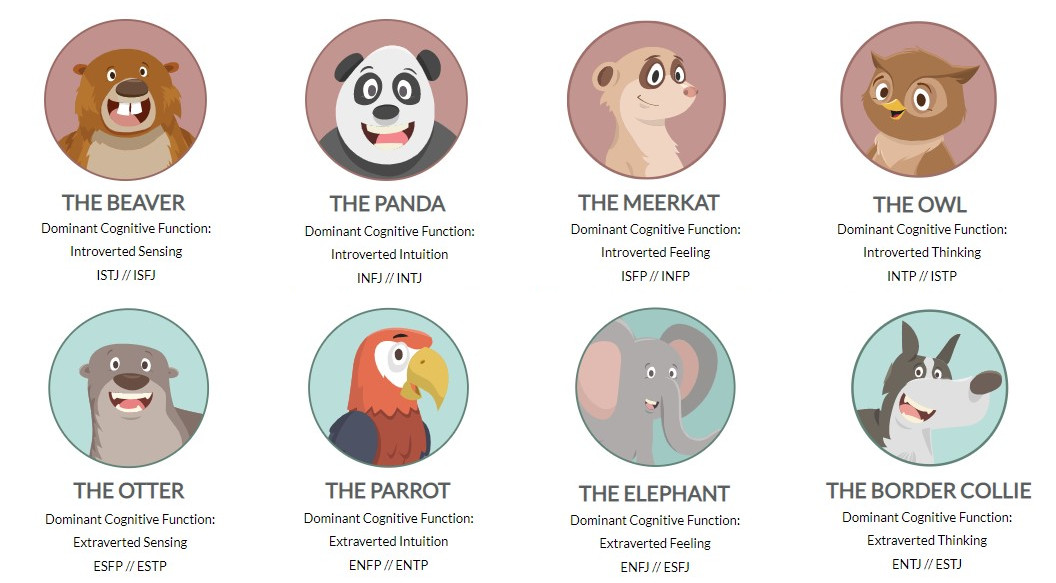
\includegraphics[width=0.4\textheight,angle=0]{img/animals}}
		\caption[Alle Tiere des Persönlichkeitstests]{Alle Tiere des Persönlichkeitstests \cite{knowAndLove}}
		\label{img:animals}
	\end{figure} 
	In der ersten Stunde der Studie mussten alle Teilnehmer den Computational Thinking Test durchführen. Die Auswertung der Ergebnisse aus der ersten Stunde jedes Teilnehmers befinden sich in Tabelle \ref{tab:data}. Wie bereits erwähnt, besteht dieser Test aus mehreren Kategorien, die normalisierten Ergebnisse befinden sich in Abbildung \ref{img:auswertung}.\\
	Die Termine der Studie können in zwei Phasen eingeteilt werden. Die erste Phase ist die Phase, in der die Kinder sich mit Lego WeDo vertraut machten. Die jeweiligen Termine hatten ein eigenes Thema, welches von der WeDo-App angeboten wurde. Die Autoren stellten zu Beginn eines Termins den Kindern Fragen zum Thema und es wurde über das Thema diskutiert. Nachdem die Diskussionsrunde vorbei war, führten die Kinder selbständig die von der WeDo-App bereitgestellten Kurse zu dem Thema durch während die Autoren die Kinder beobachteten und dabei Notizen in einem Fragebogen machten. Der Fragebogen wird im weiteren Verlauf noch genauer erklärt. Die zweite Phase läutete den Beginn des Wettbewerbs ein. Die beiden Gruppen, je vier Teilnehmer, erhielten ein sogenanntes Motivationsset von Lego, welches zusätzlich zu den bis dahin verwendeten Kästen verwendet wurden. Der Aufbau dieser Termine ähnelte dem von Phase eins: Jeder Teilnehmer bekam mit dem Motivationsset ein sogenanntes IngenieurInnen-Notizbuch (vgl. Abbildung \ref{img:explorer_heft}). In jedem Heft sind Aufgaben für die Kinder, insgesamt existieren 12 dieser Treffen, welche alle auf den Wettbewerb hinführen. Bei jedem dieser Treffen wird ein Thema, wie bereits in Phase eins besprochen, bevor die Kinder anschließend selbständig die weiteren Aufgaben lösten. Auch hier notierten die Autoren das Verhalten der Kinder und trugen dies in den Fragebogen ein. 
	\begin{figure}[htbp!]
		\centering
		\fbox{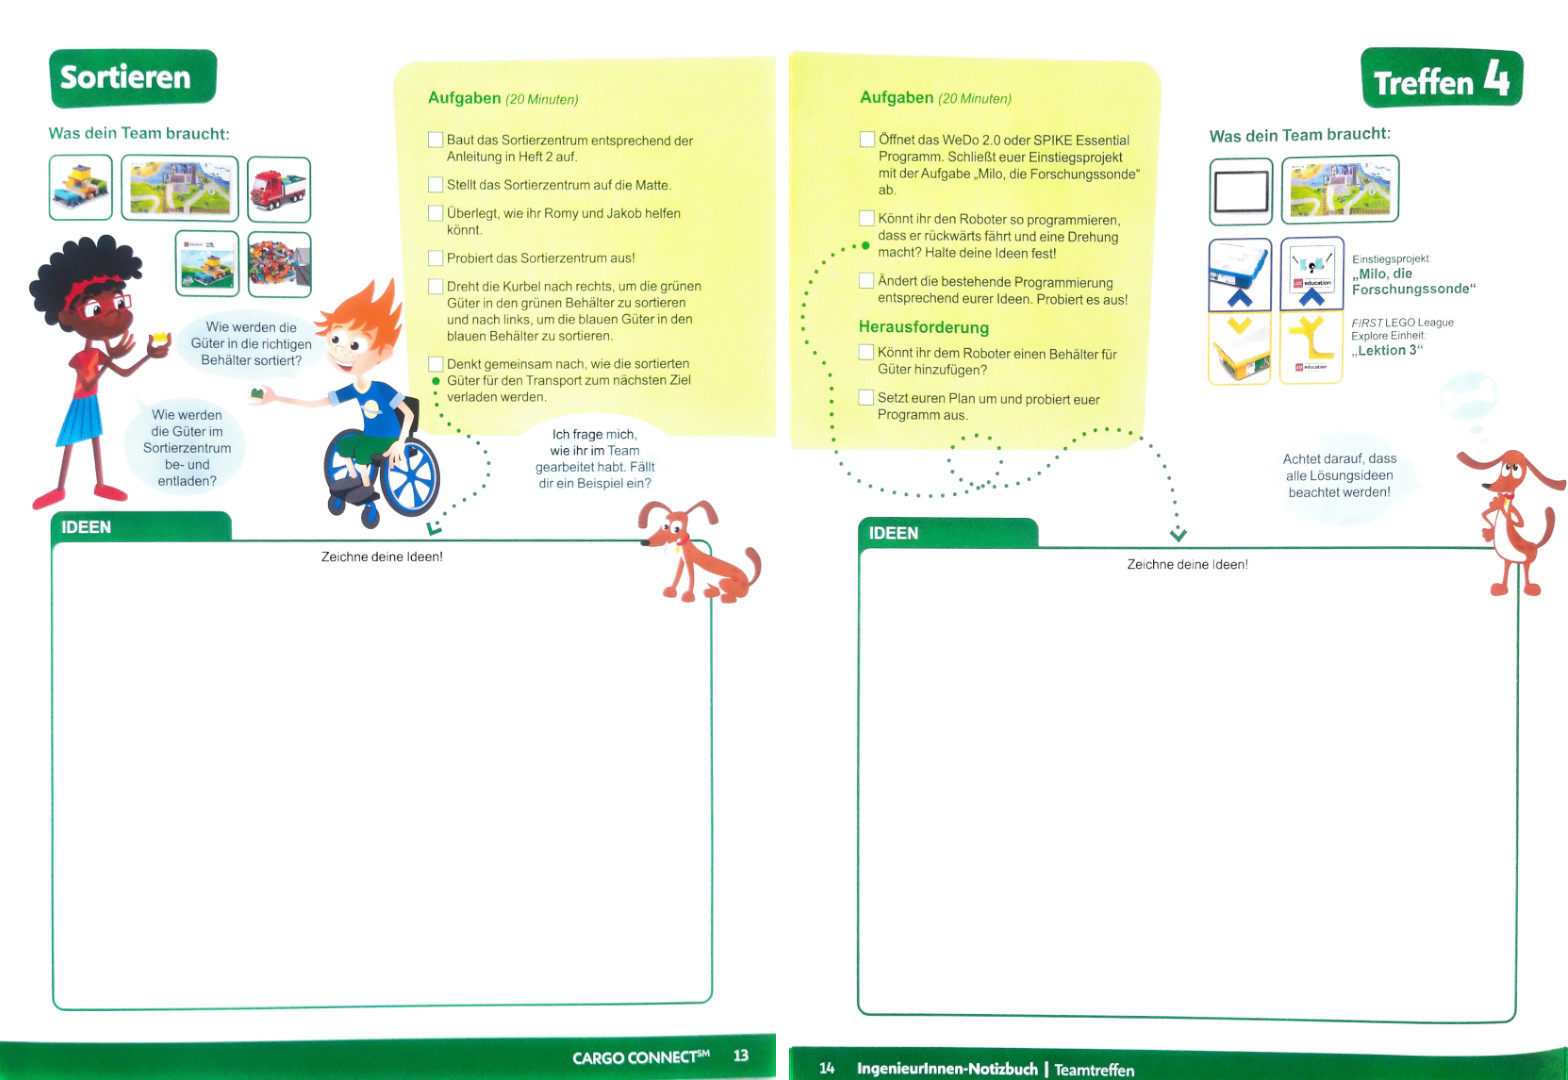
\includegraphics[width=0.3\textheight,angle=0]{img/Explorer}}
		\caption[Ausschnitt aus dem IngenierurInnen-Heft]{Ausschnitt aus dem IngenierurInnen-Heft}
		\label{img:explorer_heft}
	\end{figure}
	
\section{Ergebnisse des Computational Thinking Test}\label{sec:ErgebnisseCTT}
	\subsubsection{Vor Beginn des Workshops}
	\begin{table}[H]
		\centering
		\begin{tabular}{|
				>{\columncolor[HTML]{C0C0C0}}c |c|c|c|c|c|c|c|}
			\hline
			\textbf{Name} &
			\cellcolor[HTML]{C0C0C0}\textbf{Typ 1} &
			\cellcolor[HTML]{C0C0C0}\textbf{Typ 2} &
			\cellcolor[HTML]{C0C0C0}\textbf{Typ 3} &
			\cellcolor[HTML]{C0C0C0}\textbf{Typ 4} &
			\cellcolor[HTML]{C0C0C0}\textbf{Typ 5} &
			\cellcolor[HTML]{C0C0C0}\textbf{Typ 6} &
			\cellcolor[HTML]{C0C0C0}\textbf{Total} \\ \hline
			
		
			Henriette            & 6 & 5 & 7 & 2 & 2 & 3 & 25 \\ \hline
			Moritz               & 6 & 5 & 7 & 2 & 2 & 3 & 25 \\ \hline
			Heinz                & 6 & 5 & 7 & 2 & 1 & 3 & 24 \\ \hline
			Benny                & 6 & 5 & 7 & 2 & 0 & 3 & 23 \\ \hline
			Lulu                 & 6 & 4 & 6 & 2 & 2 & 3 & 23 \\ \hline	
			Mario                & 6 & 4 & 3 & 2 & 1 & 2 & 17 \\ \hline
			Sara                 & 6 & 2 & 7 & 0 & 1 & 1 & 17 \\ \hline		
			Jonas                & 0 & 2 & 3 & 1 & 1 & 3 & 10 \\ \hline
			\textbf{Maximalwert} & 6 & 5 & 7 & 2 & 2 & 3 & 25 \\ \hline
		\end{tabular}
		\caption{Erreichte Punkte pro Kategorie}
		\label{tab:data}
	\end{table}
	
	In der obenstehenden Tabellen sind die Anzahl der Punkte aufgeführt, die die einzelnen Teilnehmer, hier mit Pseudonym aufgeführt, erreicht haben. Wie aus der letzten Zeile deutlich wird, sind unterschiedliche Maximalpunkte erreichbar. Daher wurden für die beiden folgenden Abbildungen die Werte dieser Tabelle auf 10 normalisiert. Dabei ist zu sehen, dass besonders in Kategorie 1, welche reine Sequenzen abfragte, und Kategorie 3, die den Umgang mit verschachtelten Schleifen prüfte, fast alle Probanden außer Jonas die volle Punktzahl erreicht haben, da er die Fragen nicht eindeutig beantwortet hatte und deshalb ihm keine Punkte gegeben werden konnte.	\\ 
	
	
	\begin{figure}[H]
		\centering
		\begin{tikzpicture}
			\tkzKiviatDiagram[scale=.5,label distance=.5cm,
			radial  = 5,
			gap     = 1,  
			lattice = 10]{Typ 1,Typ 2,Typ 3,Typ 4 ,Typ 5, Typ 6}
			%Jonathan
			\tkzKiviatLine[thick,color=blue,mark=none!20,opacity=1](10,8,4.285714286,10,5,6.666666667)
			%Annabell
			\tkzKiviatLine[thick,color=green,mark=none!20,opacity=.85](10,10,10,10,10,10)
			%Luise
			\tkzKiviatLine[thick,color=yellow,mark=none!20,opacity=.5](10,8,8.571428571,10,10,10)
			%Benny
			\tkzKiviatLine[thick,color=magenta,mark=none!20,opacity=.85](8.333333333,6,4.285714286,5,0,3.333333333)
			%Mohammed
			\tkzKiviatLine[thick,color=orange,mark=none!20,opacity=.85](10,10,10,10,5,10)
			%Yufei
			\tkzKiviatLine[thick,color=brown,mark=none!20,opacity=.85](10,4,10,0,5,3.333333333)
			%Henrik
			\tkzKiviatLine[thick,color=purple,mark=none!20,opacity=.85](0,4,4.285714286,5,5,10)
			%Namenslos
			\tkzKiviatLine[thick,color=teal,mark=none!20,opacity=.85](10,10,10,10,10,10)
			%Maximalwert
			%\tkzKiviatLine[thick,color=black,mark=none,
			%fill=black!20,opacity=1](10,10,10,10,10,10)
			\tkzKiviatGrad[prefix=,unity=1](1)  
			
		\end{tikzpicture}
		\caption[Auswertung]{Auswertung der Tests}
		\label{img:auswertung}
	\end{figure}
	
	Abbildung \ref{img:auswertung} verwendet die normalisierten Werte aus Tabelle \ref{tab:data}. Sichtbar wird hier besonders der Einbruch in der Kategorie für Bedingungen mit If und Else, nur ein Proband konnte hier alle Fragen richtig beantworten. Bei Kategorie 3 ist erkennbar, dass es hier wohl große Unterschiede zwischen den einzelnen Teilnehmern gibt, da hier die Extremwerte eine Differenz von etwas unter 6 Punkten, also fast 60\% Unterschied sichtbar wird. Auch die Typen 2 und 6 weisen ähnliche Muster auf, wobei bei Typ 6 die Differenz über 6 liegt. Typ 1 und Typ 4 dagegen ist bei allen Teilnehmern fast gleich gut, hier ist die Differenz der Extremen deutlich geringer.\\ 
	
	
	
	
	
	\begin{figure}[H]
		\centering
		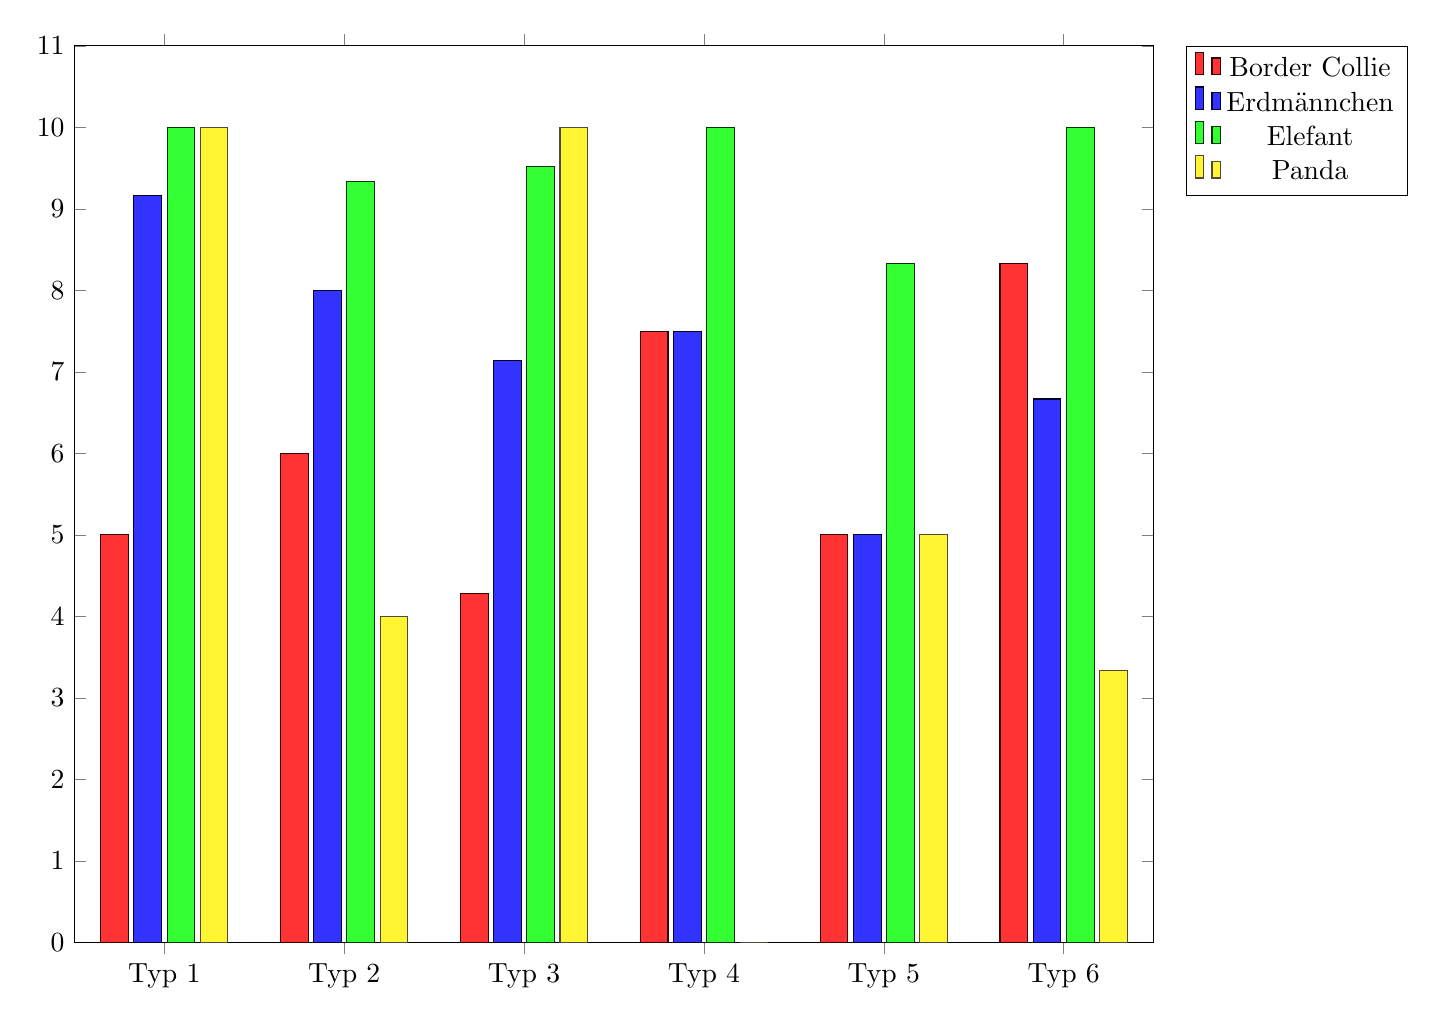
\begin{tikzpicture}
			\begin{axis}[
				ybar,ymin=0,
				symbolic x coords={Typ 1, Typ 2, Typ 3, Typ 4, Typ 5, Typ 6},xtick={Typ 1, Typ 2, Typ 3, Typ 4, Typ 5, Typ 6 
				}, scale = 2,legend pos=outer north east
				]
				%Border Collie
				\addplot[red!20!black,fill=red!80!white] coordinates
				{(Typ 1,5) (Typ 2,6) (Typ 3,4.285714286) (Typ 4,7.5) (Typ 5,5) (Typ 6,8.333333333)};
				%Erdmännchen 9,166666667	8	7,142857143	7,5	5	6,666666667
				\addplot[blue!20!black,fill=blue!80!white] coordinates
				{(Typ 1,9.16666667) (Typ 2,8) (Typ 3,7.142857143) (Typ 4,7.5) (Typ 5,5) (Typ 6,6.66666667)};
				%Elefant
				\addplot[green!20!black,fill=green!80!white] coordinates
				{(Typ 1,10) (Typ 2,9.333333333) (Typ 3,9.523809524) (Typ 4,10) (Typ 5,8.333333333) (Typ 6,10)};
				%Panda
				\addplot[yellow!20!black,fill=yellow!80!white] coordinates
				{(Typ 1,10) (Typ 2,4) (Typ 3,10) (Typ 4,0) (Typ 5,5) (Typ 6,3.33333333)};
				\addlegendentry{Border Collie}
				\addlegendentry{Erdmännchen}
				\addlegendentry{Elefant}
				\addlegendentry{Panda}
			\end{axis}
		\end{tikzpicture}
		\caption[Auswertung Durchschnitt]{Durchschn. Punkte pro Kategorie der einzelnen Typen, normalisiert}
		\label{img:auswertung_typus}
	\end{figure}

	Ebenfalls die normalisierten Werte verwendet auch Abbildung \ref{img:auswertung_typus}. Hierbei wird der Durchschnitt der einzelnen Typen pro Kategorie des Tests dargestellt. Auffallend ist besonders der Typ Border Collie und Elefant. Border Collie hat eine relativ geringe Durchschnittspunktzahl in den Testkategorien erreicht, Elefant dagegen erreichte in der Hälfte aller Kategorien den Maximalwert, in der anderen Hälfte kam dieser Typ nahe ans Maximum. Der Panda dagegen hat eine relativ hohe Streuung, die Werte liegen im kompletten Bereich von 0 bis inklusive 10.\\
	\subsubsection{Am Ende des Workshops}
	
\section{Parallelveranstaltung an der German University of Cairo}
Was wurde gemacht? \\
Wie viele Kinder --> 4 \\
Aufbau eines Kurses?\\
Alter und Beschreibungen der Kinder\\
    \chapter{Beobachtungen}
Im folgenden Abschnitt werden die subjektiven Beobachtungen der Autoren dokumentiert. Dabei werden die Beobachtungen nach Persönlichkeitstyp kategorisiert.
\section{Präsenzveranstaltungen}
\subsection{Border Collies}
Während den Workshops konnte bei allen Probanden, welche aus ihrem Persönlichkeitstest das Ergebnis \textit{Border Collie} erhielten, festgestellt werden, dass ihre Fähigkeit, im Team zu arbeiten, vorhanden war. Bei den beiden Kindern, die diesen Persönlichkeitstyp zugeordnet hatten, hat sich die Teamfähigkeit weder verschlechtert oder verbessert. Für die Kinder war das Arbeiten des Teams wichtig, sie arbeiteten miteinander und schätzen die gegenseitigen Beiträge, so dass keiner im Alleingang arbeitete. Ihr Verhalten gegenüber anderen Teampartnern war bei beiden Kindern in der Regel gleich, nur zu Beginn der Workshops zeigte ein Kind einen leicht arroganten Charakter gegenüber anderen Kindern, welcher sich durch Aussagen wie: \textit{"Mach du das mal, ich kann das schon"}, äußerte. Wenn es darum ging, die Führungsrolle zu übernehmen, konnten beide Teilnehmer gut andere Teampartner anweisen, ohne aber dabei zu dominant zu werden. Beide Kinder kommunizierten in der Regel sehr gut mit anderen Kindern, eines der Kinder hatte jedoch manchmal Schwierigkeiten, sich richtig auszudrücken. Dieses Verhalten ist vermutlich nicht auf die Persönlichkeit, sondern auf einen Sprachfehler zurückzuführen. Dasselbe Kind war jedoch trotz der Schwierigkeiten sich auszudrücken sehr kommunikativ was das Feedback betraf. Die Autoren wurden häufig gefragt, für wie gut sie die Bauwerke des Kindes befanden.


Die Kinder des Persönlichkeitstyps \textit{Border Collie} hatten jedoch Schwierigkeiten, eigene Ideen während der Besprechungsrunden zu bilden. Häufig wurden entweder Ideen von anderen Teilnehmern übernommen oder nur nach Hilfestellung der Autoren, welche das Maß, welches bei der Altersklasse angemessen wäre, übertraf, so dass häufig bei ganz niedrigen Grundlagen gestartet werden musste. Jedoch konnte manchmal auch beobachtet werden, dass die Kinder verschiedene Konzepte ausprobierten, dies allerdings geschah nur sehr selten. Die Kinder taten sich auch häufig schwer, die Dinge auch aus anderen Perspektiven zu betrachten.\\
Ein Abstraktionsverhalten der Kinder wurde kaum festgestellt, nur ganz selten konnte beobachtet werden, dass die Kinder über das Thema hinaus sehen konnten. Ihr Verhalten in den Aspekten Beharrlichkeit und Integrationsfähigkeit wurde von den Autoren als gut dokumentiert. Dies bedeutet, dass die Kinder zwar in der Lage waren, diese Fähigkeiten zu zeigen, dies jedoch nicht sehr häufig geschah oder die Ausprägung der Fähigkeiten nicht stärker war.\\
Generell konnte beobachtet werden, dass die Kinder gegenüber neuen Themen sehr offen eingestellt waren und sich dann auch mit den Themen gedanklich befassten. Ab und zu konnte festgestellt werden, dass die Kinder ein wenig Fantasie zeigten und ab und zu Züge von Humor aufzeigten. Die Kinder zeigten in der Regel sich als sehr spielerische Kinder, was sich dadurch zeigte, dass die Kinder öfters auch mit ihren Bauwerken und anderen Teilen spielten, statt diese nur zu reinen Programmierzwecken zu verwenden.\\
Die Kinder zeigten während der Workshops, besonders beim Implementieren ihrer Programme, dass sie in der Lage sind, logisch zu denken. Die logischen Gedankengänge konnten auch, wenn die Autoren die Kinder dazu befragten, erklärt werden.


Wenn es darum ging, Probleme zu beschreiben, waren beide Kinder dieses Persönlichkeitstyps in der Lage, dies zu tun. Dazu wurde keine Hilfestellung seitens der Autoren benötigt. Erfolgskriterien konnten von den Kindern nicht  selbständig genannt werden, genauso wenig konnten sie das Problem nicht in kleinere Schritte zerlegen, außer die Autoren führten sie mit Fragen durch das Problem. Hin und wieder konnte bei einzelnen Fällen erkannt werden, dass die Kinder in der Lage sind, Muster zu erkennen. Gelernte Konzepte konnten im Regelfall von den Kindern selbständig angewandt werden, ohne dass Hilfe benötigt wurde.\\
Das algorithmische Denken wurde bei den von Lego gestellten Projekten übernommen, da die Software den benötigten Code vorgab und die Kinder nur den Code nachbauen mussten. In den freien Aufgaben, die unabhängig von den genannten Projekten waren, konnten die Kinder in der Regel nachdem die Autoren ihnen den Weg gezeigt hatten, ein algorithmisches Denken an den Tag legen. Die algorithmischen Konzepte, die unter anderem in Abbildung \ref{pdf:observation_sheets} aufgeführt wurden, konnte nach einigen Wochen von den Kindern selbständig angewandt werden, ohne dass externe Hilfe benötigt wurde.\\
Durch die Vorgabe ist auch die Beurteilung der Funktionalität eines Programms hinfällig, weshalb lediglich freie Aufgaben bewertet wurden. Diese Aufgaben wurden in den meisten Fällen selbständig bearbeitet und funktionierten ohne Eingreifen der Autoren. Fehler wurden selbständig behoben, alternative Lösungen wurden jedoch zu selten gefunden, als dass dies hätte bewertet werden können.

\subsection{Elefanten}
Bei zwei der drei Kinder, bei denen der Persönlichkeitstest als Ergebnis Elefant ergab, konnte festgestellt werden, dass die Kinder in der Lage waren, gemeinsam im Team zu arbeiten. Heinz zeigte jedoch zu Beginn im Vergleich zu den anderen beiden Kinder ein eher dominierendes Verhalten gegenüber seiner Teampartner, was der Fähigkeit, im Team zu arbeiten, schadete. Während sich das Verhalten im weiteren Verlauf seltener auftrat und er besser in der Lage war, mit anderen zu arbeiten, verschlechterte sich bei den anderen Kindern die Teamarbeit. Alle drei Kinder gaben selten bzw. gar kein Feedback, lediglich Heinz fragte öfters nach Feedback, jedoch nur, um erneut nachzufragen, was er jetzt zu tun hatte. Während Heinz Probleme hatte, seine Teampartner miteinzubeziehen, konnten die beiden anderen Kinder ihre Partner miteinbeziehen, auch wenn sie manchmal etwas mehr zurückhaltender waren im Vergleich zu ihren Partnern. Jedoch verschlechterte sich dies ebenfalls im Verlaufe der Kurse. Heinz lernte im Verlauf, mit Teampartnern zu kommunizieren, was den anderen Kindern schon zu Beginn gelang. Moritz übernahm während den Kursen häufig die Rolle des Anführers, welche er gut ausübte. Lulu teilte sich die Rolle mit ihren Teampartnern, was in der Regel gut funktionierte. Heinz dagegen war eher ein Einzelkämpfer und führte sein Team nur selten an. Während sich das gegen Ende verbesserte, ließ bei den anderen beiden Kinder die Qualität ihrer Führungsrolle deutlich nach.

Alle drei Kinder waren sehr gute Ideengeber während der Besprechungen, ihre Ideen waren in der Regel immer sehr gute Einfälle. Von den drei Kindern war die Originalität von Moritz sehr gut, die anderen beiden Kinder hatten zwar eine gute, aber nicht übermäßig gute Fähigkeit, originelle Ideen zu bilden. Moritz war außerdem sehr flexibel in der Ideenbildung, während die anderen beiden eher Probleme damit hatten.Heinz hatte sehr große Probleme zu abstrahieren. Er hatte sehr große Schwierigkeiten, aus konkreten Dingen sich darunter etwas abstrakteres vorzustellen.\\
Für Moritz war Abstraktion weniger schwierig, er konnte, wenn gefordert, zu abstrahieren. Für Lulu war dies ebenfalls möglich.Das detailreiche Arbeiten war für Heinz eine große Herausforderung, durch die ganzen Termine hinweg fragte er alle fünf Minuten, was er jetzt machen soll. Moritz arbeitete dagegen sehr fokussiert an den Aufgaben und arbeitet diese auch häufig mit einem hohen Detailgrad aus. Gegen Ende wurde dies jedoch weniger. Lulu arbeitete in der Regel mit einem gewissen Detailgrad, welcher zwar nicht sehr hoch war, jedoch trotzdem noch ein gutes Maß an Details aufwies.Die Fähigkeit zu integrieren war unterschiedlich ausgeprägt. Moritz gelang es oft, Verbindungen zwischen einzelnen Dingen zu knüpfen, Lulu konnte dies ebenfalls genauso gut gut. Nur Heinz hatte Schwierigkeiten, auch teilweise einfache Verbindungen zu knüpfen.\\
Zu Beginn der Termine war Moritz sehr offen gegenüber neuen Themen, zeigte oftmals auch ein sehr großes Interesse an weitergehenden Einblicken in die Themen. Zudem kam ein großer Verbesserungsdrang für seine Bauwerke und wollte dafür Wissen von den Autoren. Lulu war ebenfalls sehr offen gegenüber Neuem, wenn auch nicht so aufgeschlossen wie es Moritz war. Bei beiden Kindern zeigte sich gegen Ende jedoch ein Trend, bei dem sich ihre Offenheit immer weiter reduzierte und sie Projekten weniger offen waren. Bei Heinz dagegen war eine konstante Skepsis gegen neue Themen bemerkbar. Er hatte häufig Probleme, sich in die neuen Themen einzuarbeiten. Alle drei Kinder zeigten hier und da Humor. Für zwei der drei Elefanten war es keine große Schwierigkeit, Fantasie zu zeigen, für Heinz jedoch war es teilweise schon sehr schwierig bestehende Konzepte zu bestehen.\\
Bei Moritz war das logische Denken in der Regel gut, bei den anderen beiden Kindern eher durchwachsen.

Moritz konnte meistens die Problematiken der behandelten Themen gut definieren. Wenn man ihm half, wie er die Erfolgskriterien finden kann, konnte er diese nennen. Das Zerlegen der Probleme benötigte am Anfang wenig Hilfe, gegen Ende mussten die Autoren hier und da Unterstützung bieten. Wie Moritz konnte auch Lulu die Probleme in den Workshops definieren. Bei den Erfolgskriterien konnte nichts beobachtet werden, das Zerlegen in kleinere Teile dagegen konnte mit Hilfe durchgeführt werden. Heinz zeigte beim Nennen und Zerlegen eines Problems sowie beim Nennen eines Erfolgskriteriums große Defizite, war aber nach etwas längerer und intensiverer Hilfe seitens der Autoren doch in der Lage, Genanntes durchzuführen.\\
Muster und Konzepte, die aus vorherigen Terminen bekannt waren, wurden von Heinz oftmals nur nach Hilfe verstanden. Lulu benötigte zwar für Muster mehr Hilfe, konnte aber die Konzepte häufig selbständig anwenden. Moritz zeigte bei den Konzepten durch das Hinzufügen eigener Ideen, das er in der Lage war, die gelernten Konzepte zu verstehen und nicht nur anzuwenden.\\
Im Bereich des algorithmischen Denkens zeigte Lulu, dass sie in der Regel dazu fähig war, größere Schritte zu definieren und sie in kleineren Schritte zu zerlegen. Algorithmische Konzepte wie Schleifen waren für sie nach anfänglicher Einlernphase kein Problem. Heinz hatte dagegen mehr Probleme, die großen Schritte zu definieren. Das Implementieren lief in der Regel selbständig ab, auch wenn er Probleme hatte mit Schleifen oder Ähnlichem. Für Moritz hingegen war es nicht sehr schwierig, die Schritte selbständig zu definieren und implementieren, in einigen Fällen ergänzte er die Implementierungen mit eigenen Ideen. Mit den Konzepten des algorithmischen Denkens konnte er ebenfalls meist selbständig umgehen.\\
Da wie bereits erwähnt Lego einen Teil der Programmierung abnahm, konnte für die Evaluation nur eine beschränkte Beobachtung durchgeführt werden. Die freien Programme der Kinder funktionierten meist selbständig, ohne dass Hilfe notwendig wurde. Fehler wurden von den drei Kindern ebenfalls selbständig behoben. Moritz und Lulu waren in der Lage zu erklären, warum ihr Programm jetzt genau das macht, was es sollte, während dies bei Heinz nicht beobachtbar war. Alternative Lösungen waren selten gefordert, wenn sie gefordert wurden war meist Hilfe notwendig.\\
Für den letzten Aspekt des Computational Thinking, der Abstraktion, konnte Moritz die wichtigsten Details sowohl von der Lösung als auch generell nennen. Wenn gefragt, konnte er den Autoren selbständig erklären, wie das Erfolgskriterium mit der Lösung zusammenhängt. Heinz benötigte auch für die Abstraktion sehr viel Hilfe, das Nennen der Details gelang oftmals nur nach Hilfe der Autoren, genauso wie das Knüpfen eines Zusammenhangs zwischen Lösung und Erfolgskriterien.  Lulu konnte meistens die Details selbständig nennen, nur mit den Zusammenhängen hatte sie manchmal Schwierigkeiten, sodass größere Hilfe notwendig war.

\subsection{Erdmännchen}
Die Kinder des Persönlichkeitstyps Erdmännchen konnten zu Beginn sehr gut in einem Team arbeiten, egal ob in Zweier- oder Viererteams. Beide unterscheiden sich jedoch in ihrer Rolle in einem Team. Benny zeigte sehr dominantes Verhalten in seinen Teams, selbst mit anderen Kindern, die ähnlich dominant waren. Henriette dagegen hatte ein eher zurückhaltendes Verhalten im Vergleich zu Benny. Trotz der Zurückhaltung beteiligte sie sich aktiv in den Gruppen, jedoch nicht in der Rolle einer (dominanten) Anführerin, wie es Benny häufig übernahm. Beide waren jedoch in der Lage, gut in ihren Teams zu arbeiten. Zwischen ihren Teampartnern kam es meist immer zu viel guter und sinnvoller Kommunikation. Auch bei Aufgaben, bei denen ihnen absichtlich das Gegenteil ihrer präferierten Rolle zugewiesen wurde, hatten sie keine Probleme, wenn auch es gerade für Benny schwer viel, jemand anderem seine gewohnte Rolle zu überlassen. In ihren Gruppenarbeiten wurden ihre Teampartner von ihnen immer gut unterstützt.

Auch bei den Ideen unterschieden sich beide Kinder. Benny brachte sich während den Besprechungsrunden über die verschiedenen Themen häufig ein, zeigte dabei auch verschiedene Perspektiven auf. Henriette dagegen zeigte eher weniger Flexibilität und war auch häufig abgelenkt. Ideen von beiden Kindern waren oft sehr originell und sehr kreativ, gerade Benny zeigte hin und wieder mit Ideen, welche über dem Niveau, welches in der Altersklasse normal wäre, lagen, dass er über ein hohes Maß an Wissen und Verständnis verfügte. Hier wurden physikalische Konzepte wie Reibung und Anpressdruck erwähnt, welche für dieses Alter nicht selbstverständlich sind.\\
Im Bereich des emergierenden Denkens fehlte Henriette die Fähigkeit, aus konkreten Dingen zu abstrahiern. Dies gelang Benny deutlich besser. Auch war ein deutlicher Unterschied in der Beharrlichkeit beider Kinder zu sehen. Benny arbeitete deutlich beharrlicher an den einzelnen Projekten, deutlich detaillierter als es bei Henriette der Fall war. Bei ihr trat das Problem auf, dass sie sich oft zu sehr zu leicht ablenken ließ. Während Benny auch meist ohne größere Mühe zwischen Dingen Verbindungen knüpfen konnte, waren dieselben Verbindungen für Henriette öfters nicht verständlich. \\
Bei Benny zeigte sich schon zu Beginn ein großes Interesse in die Themen und war immer sehr aufgeschlossen gegenüber neuen Themen und Konzepten. Er versuchte Unbekanntes zu verstehen und nicht nur wie es anzuwenden war. Henriette versuchte sich ebenfalls in neue Thematiken einzuarbeiten, jedoch nicht so aktiv wie es Benny versuchte. Benny, der von Anfang an sehr aktiv und redefreudig war, zeigte hin und wieder fantastische und humoristische Züge. Im Gegensatz zu ihm war Henriette deutlich schüchterner als er, welches sich aber im Laufe der Termine immer besserte. Sie verhielt sich auch deutlich kindlicher und verspielter, als es Benny tat. Auch sie zeigte, dass sie durchaus in der Lage war, mit Fantasie umzugehen. Dies wurde beispielsweise dadurch ersichtlich, dass sie in Bauwerke, welche nur aus wenigen Elementen bestanden, viele Dinge hineininterpretieren konnte.\\
Während den einzelnen Aufgaben zeigte sich, dass Benny oftmals besser in der Lage war, logische Schritte zu durchlaufen, während bei Henriette oftmals Verbindungen und Struktur fehlten.

Beide Kinder waren in der Lage, Probleme zu beschreiben, sobald sie darauf angesprochen wurden, ohne dass sie Hilfe benötigten. Es war möglich, sie nach den Kriterien zu fragen, die benötigt wurden, um die Probleme zu lösen. Lediglich die Zerlegung gelang Benny besser als Henriette.\\
Benny konnte Muster selbständig erkennen, während Henriette zwar auch in der Lage dazu war, jedoch dazu eine Hilfestellung seitens der Autoren benötigte. Nach anfänglichen Einführungen fiel es für beide Kinder leicht, bereits gelernte Konzepte in neuen Projekte umzusetzen.\\
Im Bereich algorithmischen Denken tat sich Benny sehr leicht, die Sequenzen von Schritten zu bilden und einzelne Schritte zu implementieren, während bei Henriette oft die Autoren eine Hilfestellung geben mussten. Die Konzepte wie If-Bedingungen und Ähnliches konnten sie selbständig in die Aufgaben miteinfließen lassen, nachdem sie diese erklärt bekommen haben.\\
Wie bereits erwähnt konnten die geführten Lego-Projekte selbständig gelöst werden. Bei den eigenen Projekten konnten die Programme selbständig funktionsfähig gemacht werden, auch auftretende Probleme wurden von den Kindern ohne weitere Hilfestellungen gelöst. Auf die Frage, warum dadurch das Ausgangsproblem gelöst wurde, konnten sie in der Regel ohne Führungshilfen oder andere Hilfestellungen der Autoren beantworten.\\
Während Benny selbständig die wichtigsten Details der Lösung aufzeigen konnte, war Henriette auf die Unterstützung durch die Autoren angewiesen, konnte aber dadurch ebenfalls die Details nennen.\\

Gegen Ende der Termine verschlechterte sich jedoch bei beiden die Leistung. Ihre Gruppen, die bisher immer sehr stark waren und gute Ergebnisse lieferten, hatten große Probleme, fertig zu werden und sinnvolle Aufgaben zu erledigen. Die Kommunikation untereinander verstummte, stattdessen wurde sehr viel mit anderen Gruppen geredet über Thematiken, die nichts mit den Workshops zu tun hatten. Ein Einschreiten der Autoren reduzierte zwar für kurze Zeit diesen Austausch, jedoch nach einiger Zeit nahm dieser Effekt wieder ab. Zusätzlich zu diesen Gesprächen wurden beide Kinder lauter, riefen viel durch den Raum und rannten durch den Hörsaal, in dem der Workshop stattfand. Dadurch störten sie einerseits ihren eigenen Fortschritt als auch den anderer Gruppen. Die Gruppen der beiden Kinder wurden deshalb am Ende oft nur knapp, teilweise sogar gar nicht fertig mit Aufgaben, deren Zeitaufwand deutlich weniger Zeit erforderte, als sie für die Aufgabe bekommen hatten.\\
Benny wurde gegen Ende gemeiner, versuchte Bauwerke anderer Gruppen zu zerstören, die zwar nicht für die eigentliche Aufgabe wichtig war, diese Gruppe in dieses Objekt jedoch sehr viel Fantasie steckte. Daher war hier ein Einschreiten der Autoren deutlich häufiger erforderlich.

\subsection{Panda}
Die folgenden Beobachtungen sind nur für eine Person. Daher kann es vorkommen, dass Personen, welcher dem gleichen Persönlichkeitstyp angehören, andere Verhaltensmuster aufweisen.

Das Kind, welches diesem Persönlichkeitstyp zugeordnet wurde, tat sich sehr schwer, was die Arbeit im Team anbelangt. Generell war zu beobachten, dass dem Kind die Arbeit im Team wichtig war, jedoch auch nicht allzu wichtig. Was das Lernen im Team betrifft, ist es sehr schwer, hierzu eine Beobachtung durchzuführen. Sara zeigte im Wesentlichen keine größeren Fortschritte in den Bereichen, die in den Workshops den Kindern vermittelt wurden. Einerseits arbeitete sie in einer Gruppe, wurde aber von den anderen Teilnehmern immer stark dominiert, so dass sie sich sehr zurückgezogen hatte. Die Autoren mussten hierbei sie immer wieder auffordern, an den Projekten auch geistig teilzunehmen und nicht nur zuzusehen. Durch die Zurückgezogenheit leidet auch ihre Fähigkeit zu kommunizieren, da kaum Kommunikation stattfindet und sie nicht nach Feedback fragt beziehungsweise gibt. Aufgrund ihrer rezessiven Verhaltensweise war Sara nicht in der Lage, in einer Gruppe als Führungskraft aufzutreten und andere Gruppenmitglieder zu delegieren. Trotz ihrem Verhalten konnten gegen Ende Verbesserungen im Teamverhalten beobachtet werden, was durch eine regere Mitarbeit in den Projekten sichtbar wurde.

Sara zeigte während der Workshops nur selten einen Drang zu Neuem. Zwar versuchte sie, hin und wieder dabei zu sein, hatte aber sonst damit oft Probleme. Für ihre emotionale Sensitivität kann nur eine Aussage über ihre Schüchternheit getroffen werden. Dadurch zeigte Sara während den Workshops nur selten bis gar nicht, dass sie die Fähigkeit für Humor besitzt. Bei den Bauwerken und Ideen konnte sie ab und zu ein wenig Fantasie zeigen, aber ansonsten blieb diese Eigenschaft im Verborgenen.\\
Das logische Denken konnte durch ihre geringe Mitarbeit nur bei Aufforderung beobachtet werden, jedoch fiel ihr logische Schlüsse zu ziehen schwer.

Generell kann über ihre Computational Thinking Skills gesagt werden, dass sie für die meisten Attribute zwar in der Lage war, jedoch nur nach Aufforderung und zeigen durch die Autoren. Mithilfe von Hilfestellungen und dem Führen durch Probleme und Themen war sie dann doch in der Lage ein Problem zu zerlegen und zu erkennen, was nötig ist, um dieses Problem zu lösen. Dasselbe galt auch für bereits gelernte Konzepte; Sara musste oft noch einmal an die Konzepte, die in den letzten Stunden durchgearbeitet wurden, herangeführt werden.\\
Wie bei den anderen Gruppen bereits erwähnt, wurden für das algorithmische Denken nur die freien Aufgaben abseits der geführten Kurse beobachtet. Hier hatte Sara jedoch einige Probleme, stand auch hier wieder im Schatten ihrer Teampartner, welche das meiste für sie erledigten. Zwar haben die Programme ihres Teams funktioniert, ihre Mitarbeit an diesen ist jedoch nie sehr hoch gewesen, nur nach mehrmaligem Auffordern. Alternative Lösungen wurden nicht geboten.\\
Ihre Fähigkeiten der Abstraktion waren auch nur durch sehr viele Hilfestellungen möglich, ein Hinterfragen der Lösung warum diese jetzt funktioniert und weshalb ein Teil der Implementierung wichtig ist für die Lösung konnte sie nur sehr schwer durchführen.


\subsection{Gruppenkonstellationen}
Während den Terminen arbeiteten die Kinder oft zusammen. Die Teamauswahl erfolgte meist selbständig. Wenn die Autoren die Teams bildeten, wurde darauf geachtet, dass auch dominantere Kinder sich den Anweisungen anderer Kinder fügen müssen, beispielsweise durch konkretes Aufteilen der Aufgaben, dass ein Kind die Anweisungen geben muss und nicht bauen darf und das andere Kind die Anweisungen seines Partners ausführen muss.\\
Wenn die Kinder selbständig ihre Partner wählen durften, bildeten sich meist die folgenden Gruppen:
\begin{itemize}
	\item Benny (Erdmännchen) \& Moritz (Elefant)
	\item Henriette (Erdmännchen) \& Lulu (Elefant)
	\item Jonas (Border Collie) \& Mario (Border Collie)
	\item Sara (Panda) \& Heinz (Elefant)
\end{itemize}
Zur letzteren Gruppe muss angemerkt werden, dass diese beiden oft zusammenarbeiten mussten, weil keine anderen Teamkonstellationen mehr verfügbar waren. Alle anderen Teamkonstellation bestanden jeweils aus befreundeten Kindern.\\
In manchen Fällen war es notwendig, dass zwei Vierergruppen gebildet wurden. Die Gruppen, die sich dann bildeten, sahen wie folgt aus:
\begin{itemize}
	\item Benny (Erdmännchen) \& Moritz (Elefant) \& Henriette (Erdmännchen) \& Lulu (Elefant)
	\item Jonas (Border Collie) \& Mario (Border Collie) \& Sara (Panda) \& Heinz (Elefant)
\end{itemize}
Die Konstellationen basierten auf den Schulen, die die Kinder besuchten. Eine Gruppe bestand aus Kindern von genau einer Schule. Für den späteren Wettbewerb wurden diese beiden Gruppen in obiger Konstellation angemeldet.\\


\section{Onlineveranstaltungen}
Aufgrund der COVID-19-Pandemie wurden einige Termine online abgehalten. Dafür trafen sich die Teilnehmer und die Autoren gemeinsam in einem Online-Raum, wobei öfters zwei Kinder sich zuhause getroffen haben und dann gemeinsam in der Sitzung dabei waren. Aufgrund von Ausfällen seitens der Autoren konnte nicht aus allen Terminen Beobachtungen gewonnen werden, da der Kursleiter nicht in der Lage war, den Kindern gleichzeitig etwas beizubringen und dabei auf alle Kinder zu achten.\\

Für die Online-Sitzung mit dem Thema Forschungssonde waren Lulu und Sara abwesend.\\
Heinz arbeitet unsorgfältig an seinen Bauwerken, was zur Folge hatte, dass sein Bauwerk öfters auseinander fiel. Nur mit Hilfe der Autoren gelang es ihm, am Ende ein korrektes Modell zu bauen. Der Grund für die Instabilität war in der Anleitung, die er nicht genau gelesen hatte. Sein Programm funktionierte. Moritz und Benny arbeiten ihr Modell schnell und mit viel Freude durch, am Ende existiert ein Modell, welches funktioniert. Durch die schnelle Arbeitszeit war geplant, ihnen weiterführende Aufgaben zu geben, was jedoch aufgrund ihrer plötzlichen Abwesenheit nach der Fertigstellung ihres Modells nicht mehr möglich war. Im Vergleich zu ihrem sonstigen Verhalten war Henriette während dieser Online-Sitzung deutlich effektiver und konzentrierter. Sie musste in dieser Sitzung ohne ihre sonstige Teampartnerin Lulu auskommen. Stattdessen hatte sie eine Freundin bei sich, welche sich bisher noch nie mit Lego WeDo auseinandergesetzt hatte. Gemeinsam bauten und programmierten sie das Modell, während Henriette ihrer Freundin alles erklärte. Die beiden Kinder Jonas und Mario kamen in dieser Sitzung nur sehr langsam voran. Jonas baute unter anderem sehr viele unnötige Anbauten an ihren Roboter an, bevor sie ein lauffähiges Programm hatten. Auch wenn sie am Ende ein fertiges Programm hatten, hatten sie beim Programmieren des Roboters sehr große Schwierigkeiten.\\
%-----------------
Bei einer weiteren Sitzung mit den Thema Tiermodelle arbeiteten Benny und Moritz, Mario und Jonas sowie Henriette und Lulu zusammen. Sara arbeitete alleine, Heinz war abwesend.\\
Sara arbeitete mit ihrer Mutter zusammen, welche am Ende des Kurses den Autoren berichtete, dass Sara die Programmierarbeit alleine übernommen hatte. In Partnerarbeit stellten Benny und Moritz ihr Modell sehr schnell fertig und auch die Programmierung funktionierte ohne Probleme. Die beiden Kinder sind jedoch danach direkt abwesend, so dass ihnen keine weitere Aufgabe gegeben werden konnte. Ebenfalls schnell fertig sind Mario und Jonas. Zusätzlich zur gestellten Aufgabe erweitern sie ihr Programm mit zusätzlichen Funktionen. Bei der Gruppe von Henriette und Lulu funktioniert die Zusammenarbeit nicht sehr gut. Henriette baut selbständig nicht relevante Bauwerke und hindert so Lulu daran, ihr Modell fertig zu bekommen. Beiden fehlt jedoch der Ideenreichtum, um ihr Modell erweitern zu können. Ihr Programm funktioniert auch erst nach etwas Hilfe durch die Autoren. Lulu musste dies alleine programmieren, da Henriette abgelenkt war.\\
%-----------------
Bei der Online-Sitzung mit dem Thema Tiermodelle \RNum{2} bauten die beiden Kinder Benny und Moritz ihr Modell zügig fertig. Dabei wurde beobachtet, dass die beiden mit sehr viel Spaß und Freude an die Sache herangingen. Für ihr Modell bauten sie zusätzliche Details mit ein, wie beispielsweise Geräusche, obwohl es nicht erfordert war. Nachdem sie ihr Modell beendeten, waren sie zwar noch im Raum angemeldet, jedoch erschienen die beiden nicht mehr vor der Kamera und waren auch nicht mehr erreichbar. In der Gruppe von Lulu und Henriette herrschte während der Arbeit eine schlechte Kommunikation. Henriette arbeitete nicht sehr konzentriert an ihrem Modell, sondern war damit beschäftigt, Unfug zu treiben. Mit den anderen Teilen baute Henriette andere Bauwerke, welche nichts mit den geforderten Aufgaben zu tun hatten. Henriettes Teampartnerin Lulu musste daher alles von alleine machen, weshalb sie nur sehr langsam voran kam. Das Programmieren funktionierte bei ihr sehr gut. Mario arbeitete sehr zügig an der Fertigstellung seines Modells, hatte auch mit der Programmierung des Modells keine Probleme. Bei Heinz war erkennbar, dass ihm die Fähigkeit der Fantasie fehlt. Er hatte große Schwierigkeiten damit, das Modell, das er baute, mit dem realen Abbild zu assoziieren. Er arbeitete in einem normalen Tempo, allerdings nicht sehr sorgfältig. Dies war unter anderem daran erkennbar, dass sein Modell sehr instabil war und ständig auseinander fiel.

\section{Verhalten am Wettbewerbstag}

Beim Wettbewerb der \acrshort{fll} wurden zwei Gruppen gebildet. Die erste Gruppe bestand aus den zwei Border Collies Mario und Jonas sowie dem Panda Sara. Heinz war ursprünglich ebenfalls in dieser Gruppe, konnte aber nicht an diesem Termin teilnehmen. Die Gruppe war sehr aufgeregt während ihrer Präsentation. Sara begann als Rednerin und hatte insgesamt auch den größten Redeanteil. Die beiden anderen Kinder der Gruppe waren etwas schüchterner und hielten sich deswegen zurück.\\
Ebenfalls aufgeregt war die Gruppe der beiden Erdmännchen, Benny und Henriette, und den beiden Elefanten Moritz und Lulu. In dieser Gruppe war der Redeanteil besser verteilt, auch wenn beispielsweise Moritz den wenigsten Anteil hatte. Dafür nannte er hin und wieder Details zu ihrer Arbeit. Die Präsentation dieser Gruppe begann Benny.

\section{Beobachtungen der German University of Cairo}
Im folgenden Abschnitt werden die Beobachtungen aufgeführt, welche im Rahmen einer Parallelveranstaltung mit ähnlichem Aufbau und Inhalt aufgezeichnet wurden. Diese stammen jedoch nicht von den Autoren selbst, sondern von Mitarbeitenden der \acrlong{guc}.\\

\subsection*{Abdelrahman}
Abdelrahman bevorzugte für den ersten Termin die Alleinarbeit. Im Verlaufe der weiteren Termine verbesserte sich dies, durch das Drängen der dortigen Kursleiter akzeptierte er die Arbeit mit seinen Partnern. Am Ende war die Wichtigkeit des Teams zwar noch nicht sehr gut, aber im Vergleich zum Beginn deutlich besser. Gleichzeitig lernte er zu Beginn nicht sehr viel im Team, da er erst seine Teampartner akzeptieren musste. Nach dem ersten Termin funktionierte dies deutlich besser, er fing an, die Ideen seiner Partner zu akzeptieren. Seine generelle Fähigkeit im Team zu arbeiten konnte nur durch Drängen verbessert werden, er selbst arbeitete von sich aus nicht gerne im Team. Gegen Ende ist dies deutlich besser. Abdelrahman gab generell gutes Feedback und fragte auch sehr aktiv nach Rückmeldungen. Jedoch war es für ihn schwierig, andere in sein Team mit einzubinden. Die Ideen seiner Partner wurden gegenüber seinen eigenen Ideen wenig geschätzt, allerdings wurde dies mit der Zeit besser. Ebenso bereitete es Abdelrahman zu Beginn Probleme, die andern Mitglieder seiner Gruppe als gleichwertig anzusehen. Über den Zeitraum, in dem die Kurse stattfanden, konnte er in diesem Aspekt Fortschritte aufzeigen. Seine Kommunikation mit anderen konnte, trotz Schwierigkeiten in der Zusammenarbeit, als gut bezeichnet werden. Auch wenn Abdelrahman in der Lage war, in seiner Gruppe als Führungsperson voranzugehen, bevorzugte er es, dass dies andere Kinder übernahmen.\\

Abdelrahman war in der Lage, viele neue Ideen während den Veranstaltungen zu generieren. Er versuchte stets, dass seine Ideen sich von den Ideen seiner Partner unterschieden. Wenn man Abdelrahman dazu drängte, Ideen aus einer anderen Sichtweise zu generieren, schaffte er dies, selbständig war dies jedoch nicht möglich.\\
Für ihn war es kein Problem, zu abstrahieren. Seine Beharrlichkeit muss hierbei als besonders gut hervorgehoben werden, da die Beobachter für den ersten Termin für diese Kategorie ein "`very very very persistent"' notierten. Zu Beginn beobachteten die Kursleiter ein Verbesserungspotenzial für Abdelrahmans Integrationsfähigkeit, ab dem zweiten Termin veränderte sich dies und seine Fähigkeit wurde als gut eingestuft.\\
Abdelrahman ist zu Beginn der Kurse nicht sehr offen gegenüber Neuem, was sich aber mit der Zeit verbessert und er Neues akzeptiert. Seine emotionale Sensitivität konnte nur schlecht beobachtet werden, genauso wie Humor und Fantasie.\\
Seine Logikfähigkeiten sind vorhanden, zu Beginn denkt er ein wenig zu logisch, in den restlichen Terminen verbessert sich dies und er zeigt gutes bis sehr gutes logisches Denken.\\ 

Für die Dekomposition konnte Abdelrahman selbständig das Problem beschreiben und versteht, was das Erfolgskriterium ist. In weiteren Terminen ist er sogar in der Lage, zu den Erfolgskriterien eigene Ideen hinzuzfügen. Zudem fügt er beim Zerlegen des Problems seine eigenen Ideen hinzu.\\
Bei der Generalisierung versteht er meistens die Muster und verbessert seine Fähigkeit, gelernte Konzepte nicht nur anzuwenden, sondern auch durch eigene Ideen zu verbessern.\\
Abdelrahman zeigte während den Terminen, dass er in der Lage war, eine Abfolge größerer Schritte zu definieren und einzelne Schritte zu implementieren. Algorithmische Konzepte verstand er aber erst während des letzten Termins.\\
Seine Programme funktionierten immer ohne Hilfe, Probleme wurden selbständig von ihm gelöst. Zudem konnte er alternative Lösungen präsentieren und erklären, warum seine Lösung das Ausgangsproblem löste.\\
Über die ganzen Termine hinweg war Abdelrahman in der Lage, das wichtigste Segment der Lösung sowie das wichtigste Detail zu nennen. Zudem konnte er ohne Hilfe erklären, wie die Lösung mit dem vorher definierten Erfolgskriterium zusammenhängt.\\

\subsection*{Farid}
Für Farid war das Arbeiten mit seinem Teampartner sehr wichtig. Jedoch war für ihn sehr wichtig, dass sein Teampartner eine bestimmte Person ist, ansonsten war er gegenüber Teamarbeit nicht sehr offen. Dies verbesserte sich im Laufe der Zeit, so dass er andere Partner akzeptierte. Generell war er jedoch in der Lage, in der Gruppe mehr zu lernen als alleine und war, trotz der Skepsis gegen anderen Teampartnern, fähig, im Team zu arbeiten. Es wurde beobachtet, dass er gutes Feedback gab und auch konstant nach Rückmeldungen von anderen Personen fragte. Farid versuchte, andere Personen in seine Gruppe mit einzubinden, für die Beobachter war es auch wichtig zu notieren, dass er die anderen Gruppenmitglieder respektierte. Der Einschätzung der Beobachter nach ist Farid ein sehr guter Kommunikator. Seine Rolle in Gruppen ist weniger die Führungsrolle, sondern eher die Rolle, bei der er die Anweisungen der Führungsperson durchführt. Führen selbst kann Farid nicht sehr gut.\\

Wenn es um das Generieren von Ideen geht, ist Farid in der Lage, sehr viele Ideen zu generieren. Diese sind allerdings nicht immer strukturiert und der Gedankengang ist nicht immer nachvollziehbar. Seine Ideen sind zwar häufig Nachahmungen anderer Ideen, jedoch versucht Farid, die Ideen mit seinen eigenen Ideen abzuändern. Generell ist er auch sehr flexibel, was Ideen angeht, auch wenn er dafür etwas Hilfe benötigt.\\
Farid zeigte während den Terminen ein sehr detailliertes Arbeiten, auch wenn das Erkennen des höheren Zieles dadurch etwas schlechter wurde. Deshalb musste er dafür etwas mehr geführt werden. Auch Farid arbeitete sehr beharrlich an den Projekten. Die Fähigkeit zu integrieren konnte bei ihm beobachtet werden.\\
Farid zeigte nach Überzeugungsarbeit sich offen gegenüber Neuem, gegen Ende öffnete er sich von selbst ein wenig mehr den Ideen und Vorschlägen anderer. Bei Farid zeigte sich ein guter Sinn für Humor. \\
Beim ersten Termin wurde bei Farid ein sehr gutes logisches Verhalten dokumentiert, der Auffassung der Beobachtenden nach müsste Farid in weiteren Terminen mehr gefordert werden. Im weiteren Verlauf wurde dies nicht mehr benötigt.\\

Bei den Computational Thinking Skills zeigte Farid, dass er in der Lage war, ein Problem zu beschreiben, die Erfolgskriterien zu benennen und das Problem in kleinere Schritte zu zerlegen. Bei letzterem war auch er in der Lage, dies durch weitere, eigene Ideen zu ergänzen.\\
Muster erwähnte Farid nie, benutzte jedoch selbständig das Wissen über gelernte Konzepte und wandte dies an.\\
Ebenso selbständig konnte Farid große Schritte für die Lösung eines Problems definieren und auch kleine Schritte implementieren. Das Verständnis für algorithmischen Konzepte konnte erst am letzten Termin beobachtet werden, davor war Farid dazu nicht fähig.\\
Die Programme, die Farid erstellte, funktionierten korrekt. Probleme wurden selbständig behoben. Durch eigene Ideen ergänzte Farid alternative Lösungen und die Beschreibung, wie seine Lösung das Problem löst.\\
Die wichtigsten Details und Bauteile der Lösung konnte Farid ohne Hilfe selbständig erklären. Für ihn war es ebenfalls kein Problem, eine Verbindung zwischen der Lösung und dem Erfolgskriterium zu ziehen. 

\subsection*{Gamal}
Das Arbeiten im Team war für Gamal wichtig. Er lernte sehr gut im Team und zeigte auch, dass er durchaus fähig war, im Team zu arbeiten. Aber für ihn war es sehr wichtig, mit einem bestimmten Partner zu arbeiten, er weigerte sich, mit anderen zusammenzuarbeiten. Wenn er jedoch im Team arbeitete, respektierte er die Rollen seiner Partner. Von sich aus fragte Gamal zu Beginn nicht nach Feedback, nur nach einiger Nachfrage fragte er nach. Dies verbesserte sich, er fragte in den weiteren Terminen nach Feedback am Ende der Session. Er selbst gab jedoch gutes Feedback und konnte den Fortschritt oder aktuelle Probleme beschreiben. Seine Anstrengung, andere mit einzubinden, waren in einem guten Rahmen. Gegenüber den Ideen anderer war er skeptisch und musste erst überzeugt werden. Später verbesserte sich dies und er fragte aktiv nach den Beiträgen anderer. Alle Mitglieder wurden von ihm gleich behandelt. Ebenso verbesserte sich seine Kommunikation von einem Austausch auf Nachfrage bis hin zu einer guten Kommunikation. In den gesamten Terminen erwies sich Gamal als ein guter Anführer. \\
Gamal generiert im Verlauf der Kurse an der \acrshort{guc} sehr viele gute Ideen, welche unterschiedlich sind von den Ideen der anderen Kinder. Gegenüber der Replikation von Ideen ist er abgeneigt. Im Zeitraum der Kurse entwickelt sich seine Flexibilität, so dass er am Ende selbständig in der Lage ist, andere Perspektiven zu haben. \\
Das Kind ist sehr detailorientiert und verliert so den Überblick über das große Ganze. Im Verlaufe der Kurse verbessert sich aber diese Fähigkeit. Zudem ist er sehr beharrlich in den Projekten. Seine Integrationsfähigkeit wurde von den Beobachtern als gut beschrieben, welche konstant bleibt.\\
Gamal ist offen gegenüber Neuem und wird über den Zeitraum der Kurse offener im Bereich des Humors, so dass er am Ende als sehr humorvoll beschrieben wird.\\
Seine Logikfähigkeit bleibt während den Kursen konstant auf einem guten Niveau.\\
In fast allen Bereichen des Computational Thinkings fügt Gamal eigene Ideen hinzu, in allen andern Fällen ist er zumindest selbständig in der Lage, diese Attribute anzuwenden. Lediglich im Bereich des algorithmischen Denkens benötigt er fast bis zum Ende, um die Konzepte zu verstehen.

\subsection*{Omar}
Omar wird von den Beobachtern im Bereich des Teamworks in den meisten Fällen nur bescheinigt, dass er diese Teilbereiche zeigt, jedoch fügen sie nur wenig eigene Notizen hinzu. Lediglich sein Feedback wird zu Beginn kritisiert, was sich jedoch im Verlauf der Kurse ändert. Auch die Kommunikation zwischen Omar und den anderen Kindern verbessert sich wohl im Laufe der Zeit. Er wird jedoch von den Beobachtern an der \acrshort{guc} nicht als Führungsperson gesehen.\\
Omar entwickelt im Verlaufe der Termine eine immer höhere Anzahl an generierten Ideen. Seine Ideen sind jedoch häufig Replikate anderer Ideen, jedoch versucht er, sich zu verbessern, so dass am Ende die Verteilung von eigenen Ideen und replizierten Ideen sich verbessert. Seine Fähigkeit der Flexibilität wird jedoch als sehr gut eingeschätzt, nachdem er zu Beginn Probleme hatte.\\
Für Omar war es leichter, das Abstrakte zu erkennen und nicht die spezifischen Details. Gegen Ende wird er etwas detailorientierter, jedoch ohne die Abstraktionsfähigkeit zu verlieren. Seine Beharrlichkeit wird als durchschnittlich bezeichnet, seine Integrationsfähigkeit sehen die Beobachter auf einem guten Niveau.\\
Omar ist ein sehr offenes Kind gegenüber neuen, anderen Ideen und Ansätzen. Sein Sinn für Humor wird den Beobachtungsbögen der ägyptischen Veranstaltung nach als gut definiert.\\
Wenn es um die logische Denkfähigkeit geht, ist Omar weniger ein logisch denkendes sondern ein kreativ denkendes Kind, was sich im Verlaufe der Kurse nicht verändert.\\
Die Computational Thinking Skills von Omar sind in der Regel so ausgeprägt, dass er bei fast allen Aspekten in der Lage ist, diese selbständig anzuwenden, ohne dass Hilfe benötigt wurde. Größere Probleme bereiteten ihm jedoch das Zerlegen von Problemen, die Implementierung von Schritten und das Anwenden von Konzepten. Bis auf den letzten Aspekt verbessert sich Omar in diesen Bereichen im Verlaufe der Veranstaltung. Beim Aspekt der alternativen Lösung ist Omar am Ende in der Lage, Ideen hinzuzufügen statt nur selbständig Lösungen zu nennen.
    \chapter[Quantitative Studie]{Quantitative Studie}
\section{Durchführung}
\section{Ergebnisse des BCTt}

    \chapter{Auswertung}
\section{Auswertung der subjektiven Beobachtungen}\label{sec:auswertungSubjektiv}
Im folgenden Abschnitt wird die Auswertung der im vorherigen Kapitel beschriebenen Beobachtungen durchgeführt.
\subsection{Problemstellung}
Nach Abschluss der Beobachtungsphase der Kinder musste nun eine Grundlage geschaffen werden, so dass die Daten, die dabei gesammelt wurden, miteinander vergleichbar werden. Durch die subjektive Beobachtungen der Autoren ist die Vergleichbarkeit nicht gegeben. Daher wurde für die Studienarbeit eine Metrik geschaffen, deren Ziel es war, aus subjektiven Bewertungen Werte zu erhalten, mit welchen besser gerechnet und verglichen werden kann.
\subsection{Entwicklung einer Metrik}
Nachdem alle Daten der Kinder erfasst wurden, sowohl die der Kinder an der \acrshort{dhbw} Karlsruhe als auch an der \acrlong{guc}, wurden alle während der Beobachtung verfassten Formulierungen gesammelt. Dies wurde gemacht, um einen Überblick darüber zu gewinnen, welches Spektrum die Aussagen der Beobachter bildeten. Um aus diesen Formulierungen ein mathematisches Spektrum zu erhalten, mussten zwei Kernfragen beantwortet werden.\\
Zuerst musste geklärt werden, wie feinstufig das Spektrum sein musste. Dies hing davon ab, wie viele verschiedene Formulierungen es bei den einzelnen Antworten gab. Häufig waren jedoch die Antworten sehr überschaubar, oftmals wurde nur ein einzelnes "`yes"' oder "`no"' in den Beobachtungsbögen eingetragen, so dass die Skala, mit der später die Formulierungen in Zahlenwerte umgewandelt werden sollte, nicht sehr fein sein musste. Für die Skala wurde deshalb ein fünfstufiges System definiert. Die Skala beinhaltete einen positiven und einen negativen Teil, welche beide aus je zwei Stufen bestanden. Für die Anschaulichkeit wurde eine zweite Skala geschaffen, so dass es einfacher war, die Werte einzuteilen. Die fünf Stufen, die die Skala zur Anschauung bildeten, waren folgende: --,-,0,+,++. Die Stufe, welche als -- bezeichnet wurde, steht ganz links auf der Skala und bildet damit den schlechtesten Wert. Auf der positiven Seite bildet die Stufe mit der Bezeichnung ++ den höchsten Wert. Mit diesen Bezeichnungen ist es nun möglich, Formulierungen einzuordnen.\\
Da mit diesen Bezeichnungen jedoch noch keine arithmetischen Operationen durchgeführt werden konnte, wurde nun eine zweite fünfstufige Skala definiert. Deren Minimum ist bei 0, was auf der Anschauungs-Skala der Bezeichnung -- entspricht. Das Maximum der Skala liegt bei 4 und ist das Gegenstück zu der Stufe mit der Bezeichnung ++ auf der Anschauungs-Skala. Nachdem die Formulierungen nun in Stufen eingeteilt wurden, konnte mithilfe dieser neuen Skala aus den Beobachtungen Daten gewonnen werden, mit denen nun Vergleiche möglich sind.\\

Die zweite Kernfrage, die sich gestellt hatte, war welche Formulierung in welche Stufe eingeordnet werden muss. Hierfür wurde noch einmal das Spektrum der Beobachtungen analysiert. Durch die bereits erwähnte Häufigkeit der Formulierung "`yes"' wurde diese als Nullpunkt der Skala definiert. Für das linke Ende der Skala wurde "`no"' definiert. Auf der rechten Seite der Skala wurde keine Formulierung definiert, welche das Maximum darstellte.\\
Bei der Einteilung der restlichen Formulierungen wurde danach geschaut, ob eine Formulierung inhaltlich das Kind besser oder schlechter bewerteten als "`yes"'. Sollte es zwischen "`no"' und "`yes"' liegen, so wurde es mit einer Eins bewertet, sollte es besser sein wurde, je nach dem wie sehr positiv die Formulierung war, mit einer Drei oder der Maximalpunktzahl Vier bewertet.\\

Die definierte Skalen sind in der untenstehenden Tabelle definiert. Das Bilden der Skala wurde von einer Studentin der \acrlong{guc} übernommen, welche nur die ihr zur Verfügung gestellten Bewertungsbögen als Grundlage dafür hatte.

\begin{table}[H]
	\centering
	\begin{tabular}{|c|c|c|c|c|}
		\hline
		-- & - & 0 & + & ++ \\
		\hline
		0 & 1 & 2 & 3 & 4 \\
		\hline
	\end{tabular}
	\caption{Definierte Skala nach Reem Ayman}
\end{table}
\subsection{Verifizierung der Metrik}
\begin{figure}[H]
	\centering
	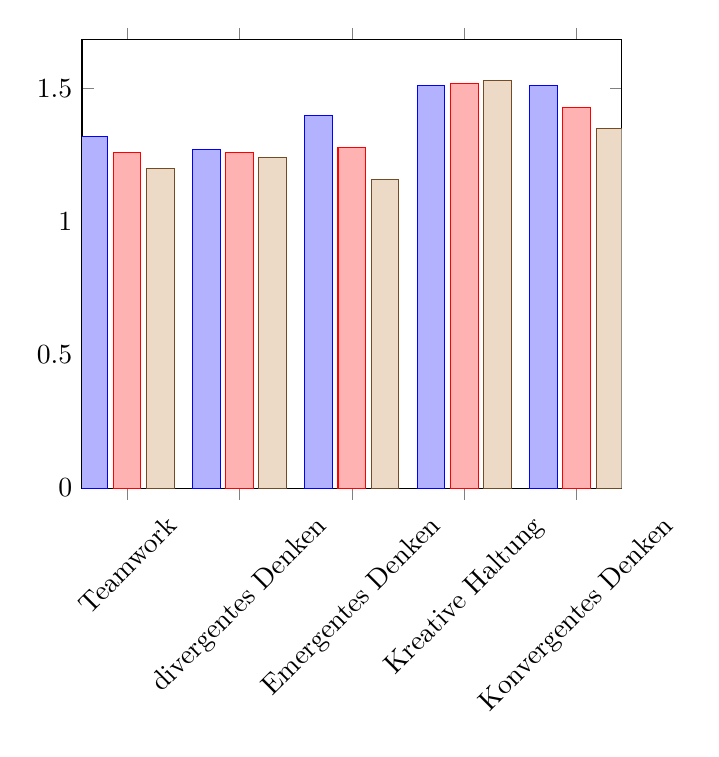
\begin{tikzpicture}
		\begin{axis}[
			ybar,ymin=0,
			symbolic x coords={Teamwork, divergentes Denken, Emergentes Denken, Kreative Haltung, Konvergentes Denken},
			xtick={Teamwork, divergentes Denken, Emergentes Denken, Kreative Haltung, Konvergentes Denken},
			xticklabel style={rotate=45}, legend style={at={(0.5,1)},
				anchor=north,legend columns=-1},
			]
			%Timo
			\addplot coordinates
			{(Teamwork, 1.32)(divergentes Denken,1.27)(Emergentes Denken, 1.4)(Kreative Haltung, 1.51)(Konvergentes Denken,1.51)};\label{diag:Timo}
			%Durchschnitt
			\addplot coordinates
			{(Teamwork, 1.26)(divergentes Denken,1.26)(Emergentes Denken, 1.28)(Kreative Haltung, 1.52)(Konvergentes Denken,1.43)}; \label{diag:average}
			%Reem
			\addplot coordinates
			{(Teamwork, 1.2)(divergentes Denken,1.24)(Emergentes Denken, 1.16)(Kreative Haltung, 1.53)(Konvergentes Denken,1.35)};\label{diag:Reem}
			
		\end{axis}
	\end{tikzpicture}

	\caption[Durchschnittliche Bewertung der Formulierungen]{Durchschnittliche Bewertung der Formulierungen zweier unabhängig voneinander bewertenden Person}
	\label{img:verificationMetric}
\end{figure}
Abbildung \ref{img:verificationMetric} zeigt wie eindeutig die von Reem Ayman definierte Metrik ist. Je weiter die beiden Balken von Timo Steidinger und Reem Ayman auseinanderliegen, umso schlechter funktioniert die Skala. Die genauen Differenzen aus der obigen Abbildung sind als durchschnittliche Abweichung in Tabelle \ref{tab:differences} aufgeführt.

\begin{table}[H]
	\centering
	\begin{tabular}{|
			>{\columncolor[HTML]{C0C0C0}}l |c|}
		\hline
		Kategorie & \multicolumn{1}{l|}{\cellcolor[HTML]{C0C0C0}durchschnittliche Abweichung} \\ \hline
		Teamwork            & 0.12 \\ \hline
		Divergentes Denken  & 0.03 \\ \hline
		Emergentes Denken   & 0.24 \\ \hline
		Kreative Haltung    & 0.02 \\ \hline
		Konvergentes Denken & 0.16 \\ \hline
		Mittlere Abweichung & 0.10 \\ \hline
	\end{tabular}
	\caption{Durchschnittliche Abweichung der beiden Bewertungen}
	\label{tab:differences}
\end{table}


\section{Entwicklung der Kinder}
\subsection{Jonas}

\begin{figure}[H]
	\centering
	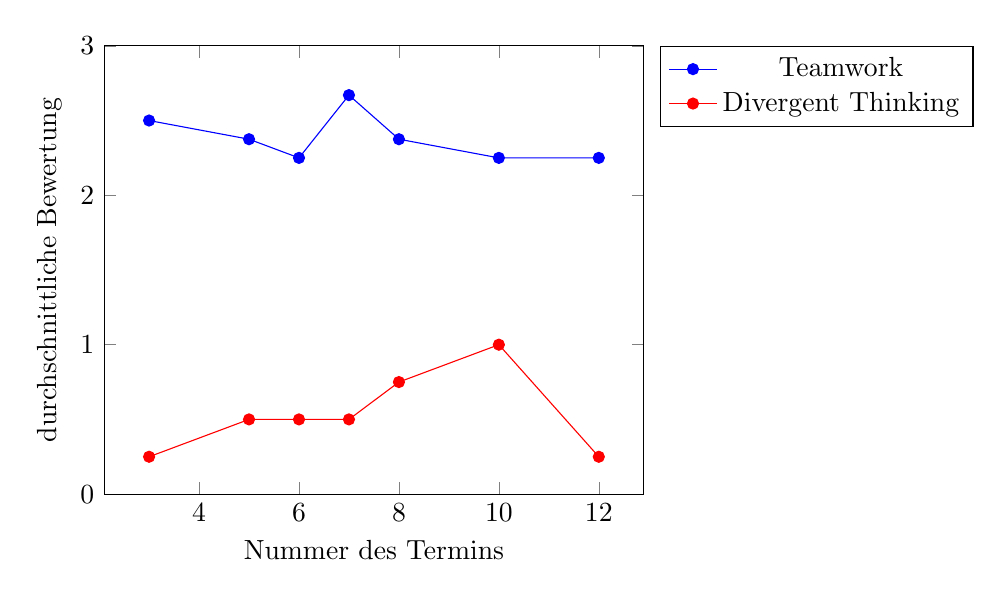
\begin{tikzpicture}
		\begin{axis}[legend pos=outer north east, ymin = 0, ymax = 3,xlabel={Nummer des Termins},ylabel={durchschnittliche Bewertung}]
			\addplot[mark=*,blue]
			coordinates {
				(3,2.5) (5,2.375) (6,2.25) (7,2.67) (8,2.375) (10,2.25) (12,2.25)
			};
			\addlegendentry{Teamwork}
			\addplot[mark=*,red]
			coordinates {
				(3,0.25) (5,0.5) (6,0.5) (7,0.5) (8,0.75) (10,1) (12,0.25)
			};
			\addlegendentry{Divergent Thinking}
		\end{axis}
	\end{tikzpicture}
	\caption{Entwicklung von Jonas}
	\label{img:jonasDevelopment}	
\end{figure}


Die Entwicklung von Jonas zeigt eine sehr konstante Teamfähigkeit. Der Durchschnitt der Bewertungen aus dem vorherigen Kapiteln wies wie in der obenstehenden Abbildung zu sehen Werte um 2.5 auf, welche damit als sehr gut einzuschätzen sind. Von einer Entwicklung im Bereich des Teamworks kann aber aufgrund seiner Konstanz nicht gesprochen werden.

\subsection{Mario}
\begin{figure}[H]
	\centering
	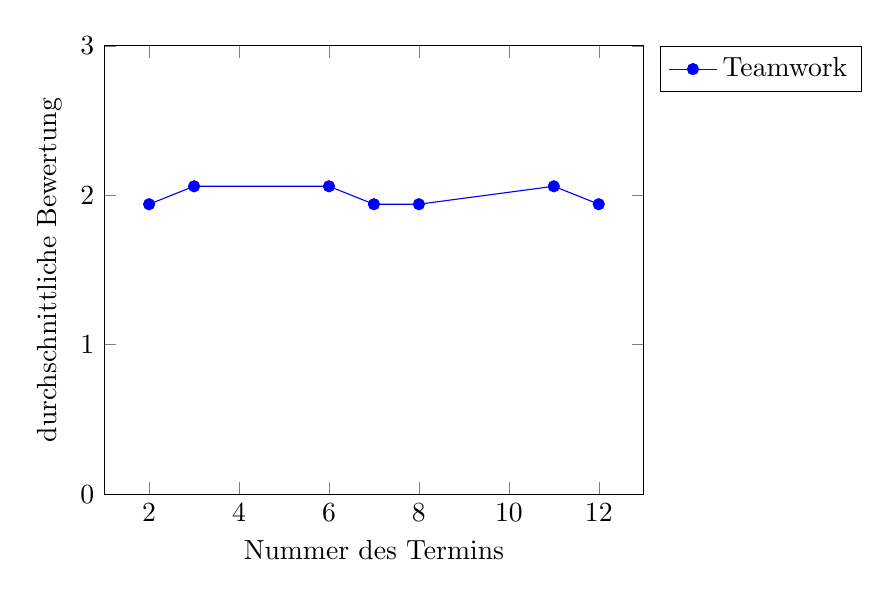
\begin{tikzpicture}
		\begin{axis}[legend pos=outer north east, ymin = 0, ymax = 3,xlabel={Nummer des Termins},ylabel={durchschnittliche Bewertung}]
			\addplot[mark=*,blue]
			coordinates {
				(2,1.94)(3,2.06)(6,2.06)(7,1.94)(8,1.94)(11,2.06)(12,1.94)
			};
			\legend{Teamwork}
		\end{axis}
	\end{tikzpicture}
	\caption{Entwicklung von Mario}
	\label{img:marioDevelopment}
	
\end{figure}



Auch Mario zeigte bei seiner Entwicklung im Teamwork nur wenig Verbesserung, dafür aber ebenfalls Konstanz. Die Differenz zwischen Maxima und Minima betragen bei ihm nur 0.12. Das bedeutet, dass auch Mario keine Entwicklung im Bereich Teamwork aufweisen kann. Generell ist seine Teamfähigkeit im oberen Mittelfeld einzuordnen.

\subsection{Sara}
\begin{figure}[H]
	\centering
	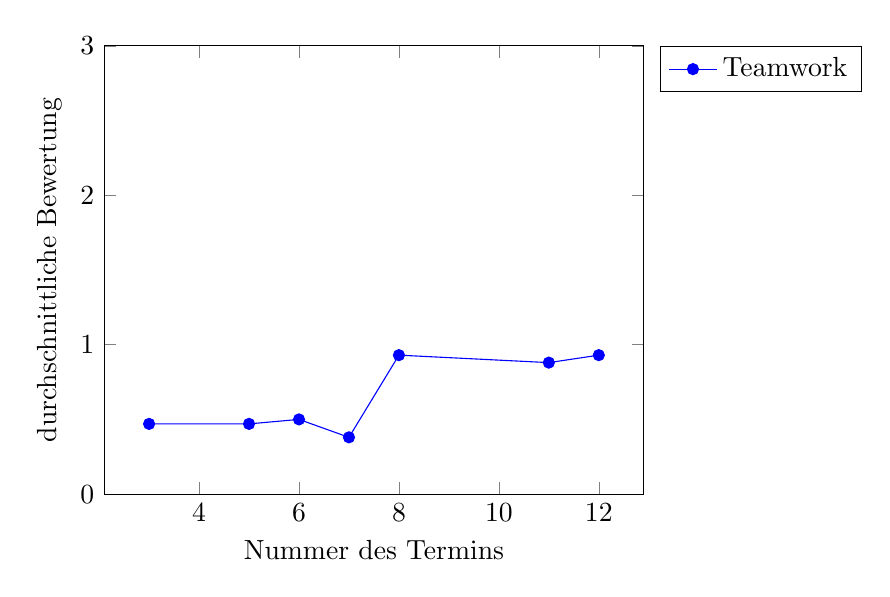
\begin{tikzpicture}
		\begin{axis}[legend pos=outer north east, ymin = 0, ymax = 3,xlabel={Nummer des Termins},ylabel={durchschnittliche Bewertung}]
			\addplot[mark=*,blue]
			coordinates {
				(3,.47) (5,.47) (6,.5) (7,.38) (8,0.93) (11,.88) (12,.93)
			};
			\legend{Teamwork}
		\end{axis}
	\end{tikzpicture}
	\caption{Entwicklung von Sara}
	\label{img:saraDevelopment}
\end{figure}

Sara zeigte im Laufe der Kurse eine starke Verbesserung ihrer Teamfähigkeit. Von anfänglich einer Bewertung von nicht einmal 0.5, zeigte Sara im weiteren Verlauf große Sprünge, so dass ihre Teamfähigkeit von den Autoren und der externen Person der \acrshort{guc} mit Werten nahe der 1.0 bewertet wurden. Für Sara ist daher eine Entwicklung im Bereich des Teamworks zu notieren.
\subsection{Benny}
\begin{figure}[H]
	\centering
	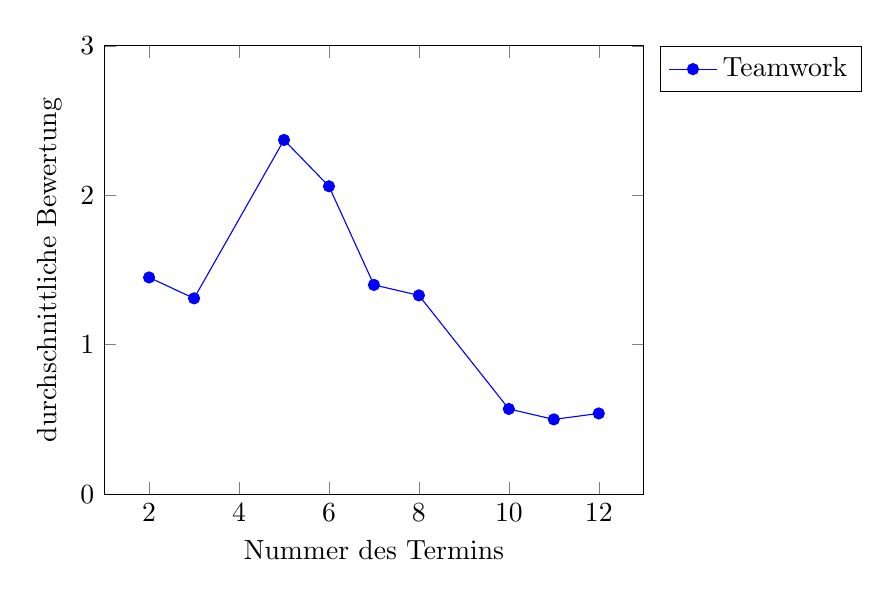
\begin{tikzpicture}
		\begin{axis}[legend pos=outer north east, ymin = 0, ymax = 3,xlabel={Nummer des Termins},ylabel={durchschnittliche Bewertung}]
			\addplot[mark=*,blue]
			coordinates {
				(2,1.45)(3,1.31) (5,2.37) (6,2.06) (7,1.4) (8,1.33) (10,.57) (11,.5)(12,.54)
			};
			\legend{Teamwork}
		\end{axis}
	\end{tikzpicture}
	\caption{Entwicklung von Benny}
	\label{img:bennyDevelopment}
\end{figure}
Zu Beginn der Kurse zeigte sich wie in Abbildung \ref{img:bennyDevelopment} zu sehen eine starke Verbesserung seiner Teamfähigkeiten, diese näherten sich dem im Vergleich zu den anderen Kindern Spitzenwert 2.5 stark an. Nachdem jedoch das Maximum erreicht war, ließen seine Teamfähigkeiten drastisch nach, so dass gegen Ende nur noch Bewertungen von etwa 0.5 erreicht wurden. Für Benny ist daher eine Entwicklung seiner Teamfähigkeit zu vermerken, eine positive Entwicklung in den ersten Terminen und am Ende eine Verschlechterung seiner Fähigkeit.



\subsection{Henriette}
\begin{figure}[H]
	\centering
	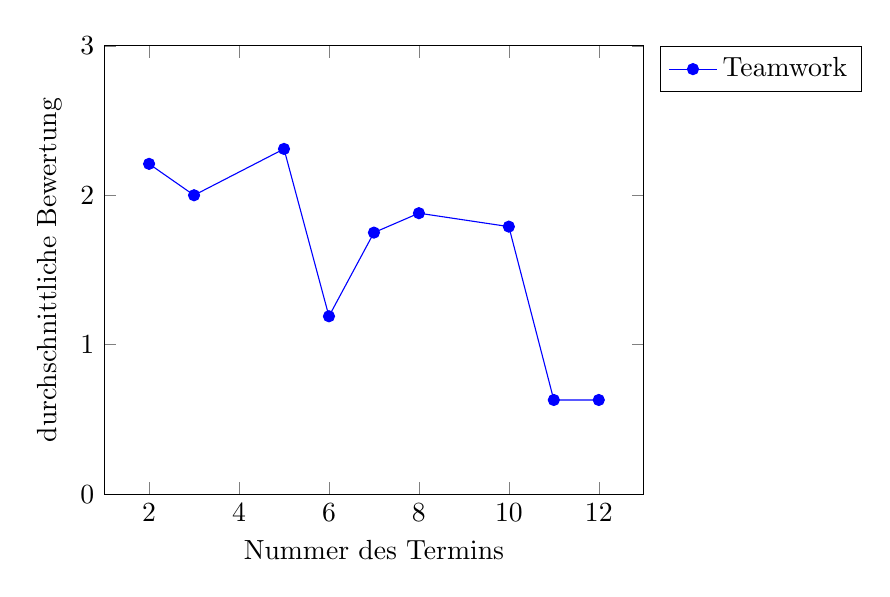
\begin{tikzpicture}
		\begin{axis}[legend pos=outer north east, ymin = 0, ymax = 3,xlabel={Nummer des Termins},ylabel={durchschnittliche Bewertung}]
			\addplot[mark=*,blue]
			coordinates {
				(2,2.21)(3,2)(5,2.31)(6,1.19)(7,1.75)(8,1.88)(10,1.79)(11,0.63)(12,0.63)
			};
			\legend{Teamwork}
		\end{axis}
	\end{tikzpicture}
	\caption{Entwicklung von Henriette}
	\label{img:henrietteDevelopment}
\end{figure}
Henriette entwickelte ihre Teamfähigkeit während den Kursen nur sehr wenig in positive Richtung. Der Durchschnitt der Bewertungen zeigte bei ihr in Abbildung \ref{img:henrietteDevelopment}, dass sie zwar eine starke Teamfähigkeit besaß, diese aber sich im Verlaufe der Kurse in eine schlechte Richtung entwickelten, so dass eine Differenz von 1.68 zwischen den Bewertungen an ihrem besten Tag und an ihrem schlechtesten Tag befindet.


\subsection{Moritz}
\begin{figure}[H]
	\centering
	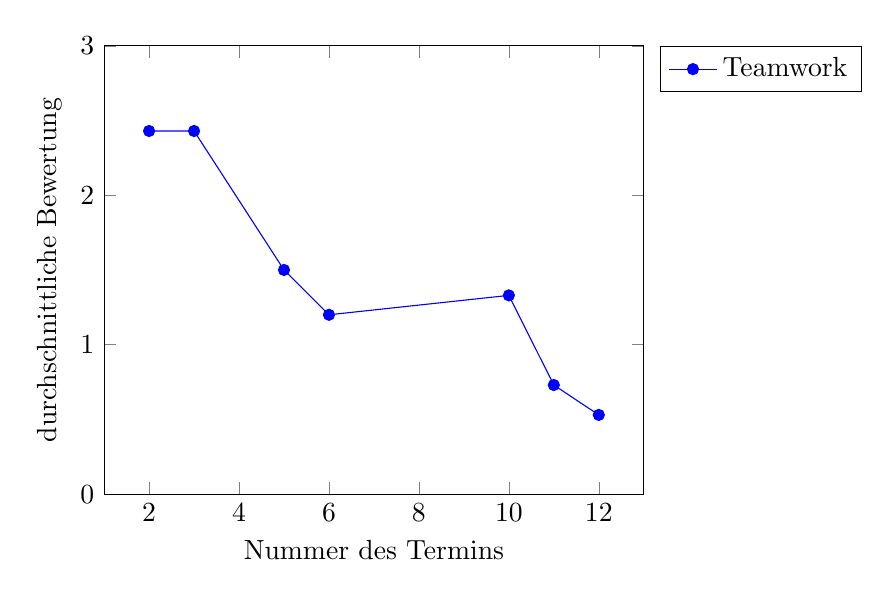
\begin{tikzpicture}
		\begin{axis}[legend pos=outer north east, ymin = 0, ymax = 3,xlabel={Nummer des Termins},ylabel={durchschnittliche Bewertung}]
			\addplot[mark=*,blue]
			coordinates {
				(2,2.43)(3,2.43)(5,1.5)(6,1.2)(10,1.33)(11,.73)(12,.53)
			};
			\legend{Teamwork}
		\end{axis}
	\end{tikzpicture}
	\caption{Entwicklung von Moritz}
	\label{img:moritzDevelopment}
	
\end{figure}
Mithilfe den Bewertungen aus Kapitel \ref{sec:auswertungSubjektiv} konnte bei Moritz ein negativer Trend festgestellt werden. Aus der obenstehenden Abbildung wird sichtbar, dass Moritz sich nicht verbessert, dafür aber in fast allen Terminen eine schlechtere Teamfähigkeit aufwies als an dem Termin davor. Seine Bewertungen für die ersten Termine lag bei 2.43, der höchste Wert von allen teilnehmenden Kindern.



\subsection{Lulu}
\begin{figure}[H]
	\centering
	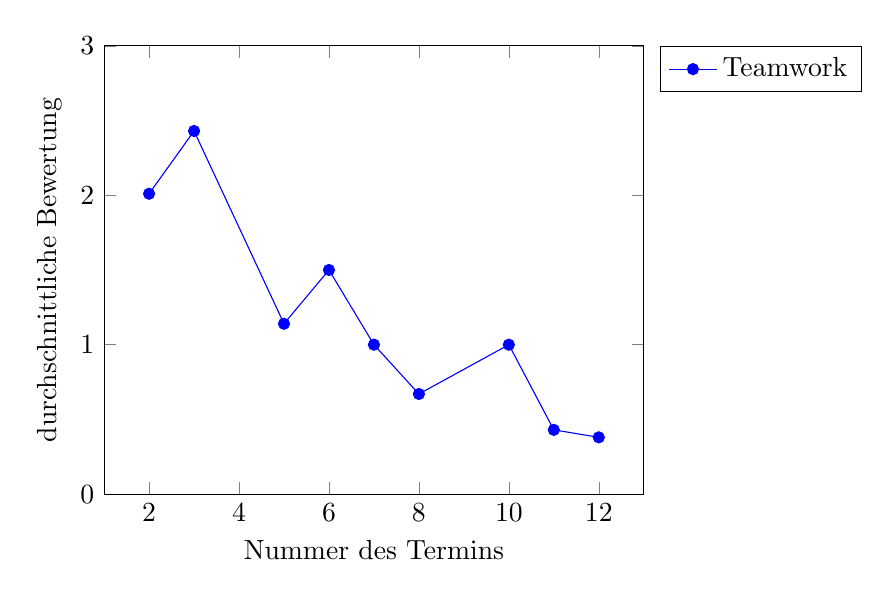
\begin{tikzpicture}
		\begin{axis}[legend pos=outer north east, ymin = 0, ymax = 3,xlabel={Nummer des Termins},ylabel={durchschnittliche Bewertung}]
			\addplot[mark=*,blue]
			coordinates {
				(2,2.01)(3,2.43)(5,1.14)(6,1.5)(7,1)(8,.67)(10,1)(11,.43)(12,.38)
			};
			\legend{Teamwork}
		\end{axis}
	\end{tikzpicture}
	\caption{Entwicklung von Lulu}
	\label{img:luluDevelopment}	
\end{figure}
Der Trend von Lulus in Entwicklung im Bereich Teamwork ist negativ. Nach einer kleinen Steigerungsphase zu Beginn, verschlechtert sich ihre Teamfähigkeit in den meisten Kursen. Hin und wieder sind Verbesserungen im Vergleich zu den voherigen Terminen sichtbar, diese knüpfen jedoch nicht mehr an die guten Leistungen im Bereich Teamwork an.



\subsection{Heinz}
\begin{figure}[H]
	\centering
	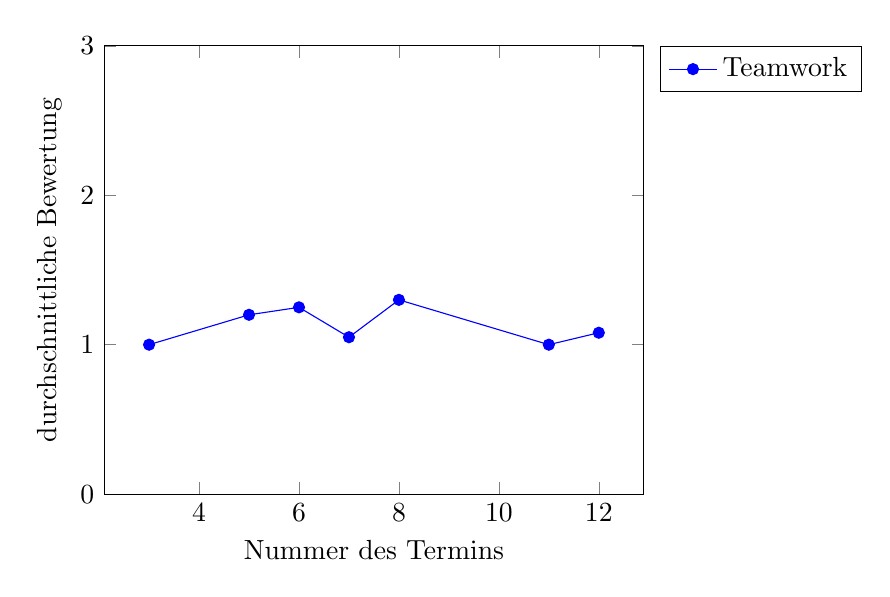
\begin{tikzpicture}
		\begin{axis}[legend pos=outer north east, ymin = 0, ymax = 3,xlabel={Nummer des Termins},ylabel={durchschnittliche Bewertung}]
			\addplot[mark=*,blue]
			coordinates {
				(3,1)(5,1.2)(6,1.25)(7,1.05)(8,1.3)(11,1)(12,1.08)
			};
			\legend{Teamwork}
		\end{axis}
	\end{tikzpicture}
	\caption{Entwicklung von Heinz}
	\label{img:heinzDevelopment}
	
\end{figure}
Während den Kursen zeigte Heinz wie in der Abbildung \ref{img:heinzDevelopment} dargestellt eine konstante Teamfähigkeit. Für ihn ist keine Entwicklung in diesem Bereich sichtbar, nur leichtere Schwankungen wurden notiert. Jedoch liegen seine Werte nur knapp über 1.0, damit liegt er sehr weit hinten im Vergleich zu den Bestwerten der anderen Kinder.


\section{Persönlichkeitstypen und Entwicklung}
\subsection{Teamwork}
\begin{figure}[H]
	\centering
	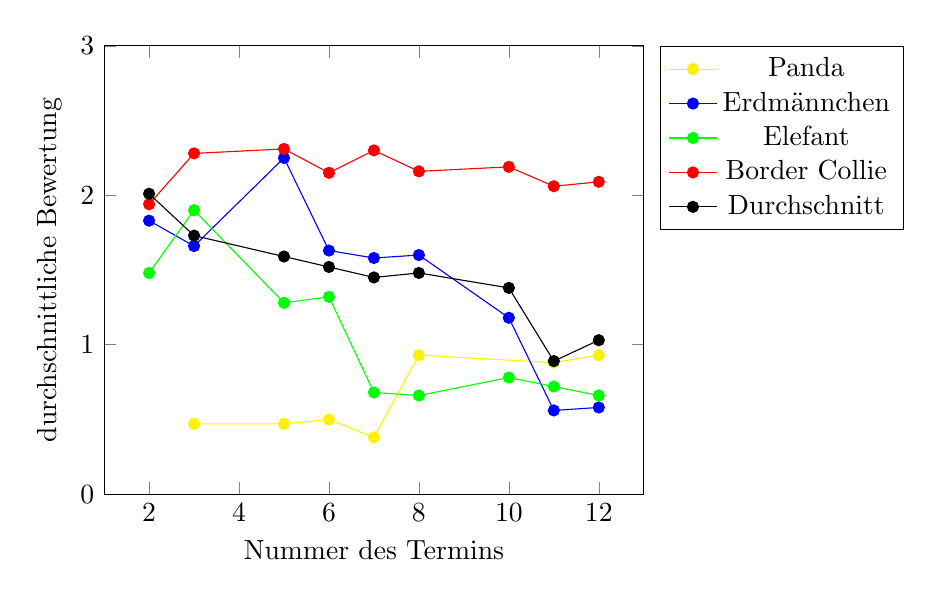
\begin{tikzpicture}
		\begin{axis}[legend pos=outer north east, ymin = 0, ymax = 3,xlabel={Nummer des Termins},ylabel={durchschnittliche Bewertung}]
			\addplot[mark=*,yellow]
			coordinates {
				(3,.47) (5,.47) (6,.5) (7,.38) (8,0.93) (11,.88) (12,.93)
			};
			\addlegendentry{Panda}
			\addplot[mark=*,blue]
			coordinates {
				(2,1.83)(3,1.66)(5,2.25)(6,1.63)(7,1.58)(8,1.6)(10,1.18)(11,.56)(12,.58)
			};
			\addlegendentry{Erdmännchen}
			\addplot[mark=*,green]
			coordinates {
				(2,1.48)(3,1.9)(5,1.28)(6,1.32)(7,0.68)(8,0.66)(10,.78)(11,.72)(12,.66)
			};
			\addlegendentry{Elefant}
			\addplot[mark=*,red]
			coordinates {
				(2,1.94)(3,2.28)(5,2.31)(6,2.15)(7,2.3)(8,2.16)(10,2.19)(11,2.06)(12,2.09)
			};
			\addlegendentry{Border Collie}
			\addplot[mark=*, black]
			coordinates{
				(2,2.01)(3,1.73)(5,1.59)(6,1.52)(7,1.45)(8,1.48)(10,1.38)(11,0.89)(12,1.03)
			};
			\addlegendentry{Durchschnitt}
		\end{axis}
	\end{tikzpicture}
	\caption{Entwicklung der Teamarbeitsfähigkeit}
	\label{img:teamDevelopment}
\end{figure}
Abbildung \ref{img:teamDevelopment} zeigt, wie sich das Verhalten der Kinder im Verlaufe der Termine entwickelt hat. Dazu wurde der Durchschnitt der Kinder eines Persönlichkeitstyps im Diagramm eingetragen. An Terminen, an denen ein Kind aufgrund Krankheit oder anderen Gründen nicht teilnehmen konnten, hatten keine Auswirkungen auf den Durchschnitt an diesem Termin, an diesen wurde dann der Durchschnitt aus den verbleibenden Kindern dieses Typs genommen.\\
Zuerst die generelle Entwicklung der Kinder der Studie. Die Fähigkeit, im Team zu arbeiten, nimmt im Verlauf des Kurses ab. Nur hin und wieder verbessert sich die Bewertungen der Kinder, jedoch nur in sehr geringem Ausmaß.\\
Da Sara das einzige Kind der Kategorie Panda ist, zeigt die obenstehende Abbildung, dass sich Pandas im Umgang mit Technologie im Rahmen der Studie ihre Teamfähigkeit verbessert haben. Da aber sie der einzige Panda der Studie ist, kann hier nicht generalisiert werden und auf andere Pandas geschlossen werden. Im Vergleich zu den anderen Kindern zeigt der Panda zwar eine Verbesserung, aber selbst das Maximum ihrer Teamfähigkeit übertrifft die Minima der anderen Kinder nur knapp und liegt durchgehend unter dem Durchschnitt. Ein Grund für das schlechte Abschneiden im Vergleich zu den Kindern kann ihre Schüchternheit sein, die während den Terminen oft an den Tag trat. Dadurch hatte sie Schwierigkeiten, sich im Team zu erweisen.\\
Die Kinder der Typen Border Collie zeigten keine Entwicklung in ihrer Teamfähigkeit, dafür ist diese jedoch im Verlaufe des Kurses konstant. An vielen Tagen haben diese Kinder eine der höchsten durchschnittlichen Bewertungen, wie aus Abb. \ref{img:teamDevelopment} hervor geht. Insgesamt ist ihre Teamfähigkeit innerhalb der Studie an der \acrshort{dhbw} Karlsruhe als überdurchschnittlich zu bewerten. Ein Grund dafür ist unter anderem die Konstanz der beiden Kinder. Bei den Teamaufgaben arbeiteten die beiden oft zusammen, die Angehörigkeit des gleichen Typs kann ein Grund für die durchgehende Konstanz ihrer Teamfähigkeit ist.\\
Die Kinder, die in ihrem Persönlichkeitstest als Ergebnis Elefant bekommen haben, verschlechterten sich in ihrer Teamfähigkeit deutlich. In den meisten Fällen ist ihre durchschnittliche Bewertung auch unterhalb des Durchschnitts der gesamten Gruppe. Grund hierfür wird vermutlich Unterforderung sein. Wie die Abbildungen \ref{img:auswertung_typus} und \ref{img:auswertung_typus_ctt} zeigen, erreichen die Kinder Höchstwerte in den einzelnen Kategorien, selbst bei dem schwierigen Test erzielten die Kinder sehr gute Ergebnisse. Für diese Kinder wäre es möglich, auch mit der nächsten Stufe der programmierbaren Roboter von Lego zu arbeiten. Die Unterforderung kann auch alterstechnisch bedingt sein. Moritz war während der Kurse bereits in der 4. Klasse und damit zwei Klassenstufen über den anderen Kindern.\\
Ebenso eine Verschlechterung zeigten die Kinder des Persönlichkeitstyps Erdmännchen. Anders als die Elefanten lag ihr Durchschnitt öfters über dem Durchschnitt aller Kinder und auch meist höher als der der Elefanten. Auch hier kann wieder als möglicher Grund für die Verschlechterung die Unterforderung der Kinder genannt werden. Erdmännchen erzielten in den Tests gute Ergebnisse und auch Benny besuchte bereits die 4. Klasse, weshalb sein Wissen und seine geistigen Fähigkeiten auf einem höheren Niveau lagen. 


\subsection{Divergentes Denken}
\begin{figure}[H]
	\centering
	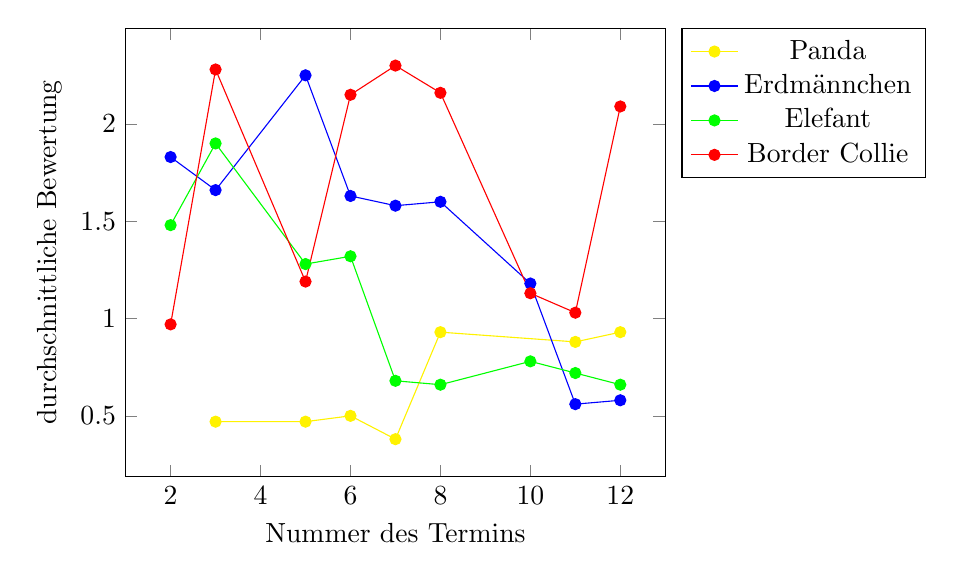
\begin{tikzpicture}
		\begin{axis}[legend pos=outer north east,xlabel={Nummer des Termins},ylabel={durchschnittliche Bewertung}]
			\addplot[mark=*,yellow]
			coordinates {
				(3,.47) (5,.47) (6,.5) (7,.38) (8,0.93) (11,.88) (12,.93)
			};
			\addlegendentry{Panda}
			\addplot[mark=*,blue]
			coordinates {
				(2,1.83)(3,1.66)(5,2.25)(6,1.63)(7,1.58)(8,1.6)(10,1.18)(11,.56)(12,.58)
			};
			\addlegendentry{Erdmännchen}
			\addplot[mark=*,green]
			coordinates {
				(2,1.48)(3,1.9)(5,1.28)(6,1.32)(7,0.68)(8,0.66)(10,.78)(11,.72)(12,.66)
			};
			\addlegendentry{Elefant}
			\addplot[mark=*,red]
			coordinates {
				(2,.97)(3,2.28)(5,1.19)(6,2.15)(7,2.3)(8,2.16)(10,1.13)(11,1.03)(12,2.09)
			};
			\addlegendentry{Border Collie}

			
		\end{axis}
	\end{tikzpicture}
	\caption{Entwicklung des divergenten Denkens}
\end{figure}	


\subsection{Emergentes Denken}
\begin{figure}[H]
	\centering
	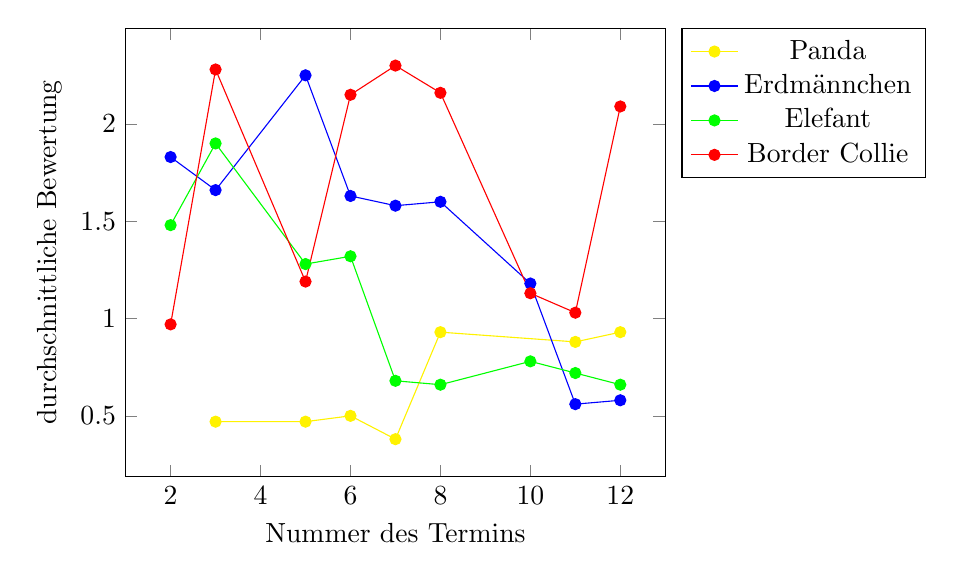
\begin{tikzpicture}
		\begin{axis}[legend pos=outer north east,xlabel={Nummer des Termins},ylabel={durchschnittliche Bewertung}]
			\addplot[mark=*,yellow]
			coordinates {
				(3,.47) (5,.47) (6,.5) (7,.38) (8,0.93) (11,.88) (12,.93)
			};
			\addlegendentry{Panda}
			\addplot[mark=*,blue]
			coordinates {
				(2,1.83)(3,1.66)(5,2.25)(6,1.63)(7,1.58)(8,1.6)(10,1.18)(11,.56)(12,.58)
			};
			\addlegendentry{Erdmännchen}
			\addplot[mark=*,green]
			coordinates {
				(2,1.48)(3,1.9)(5,1.28)(6,1.32)(7,0.68)(8,0.66)(10,.78)(11,.72)(12,.66)
			};
			\addlegendentry{Elefant}
			\addplot[mark=*,red]
			coordinates {
				(2,.97)(3,2.28)(5,1.19)(6,2.15)(7,2.3)(8,2.16)(10,1.13)(11,1.03)(12,2.09)
			};
			\addlegendentry{Border Collie}
			
		\end{axis}
	\end{tikzpicture}
	\caption{Entwicklung des emergenten Denkens}
\end{figure}	


\subsection{Kreative Haltung}
\begin{figure}[H]
	\centering
	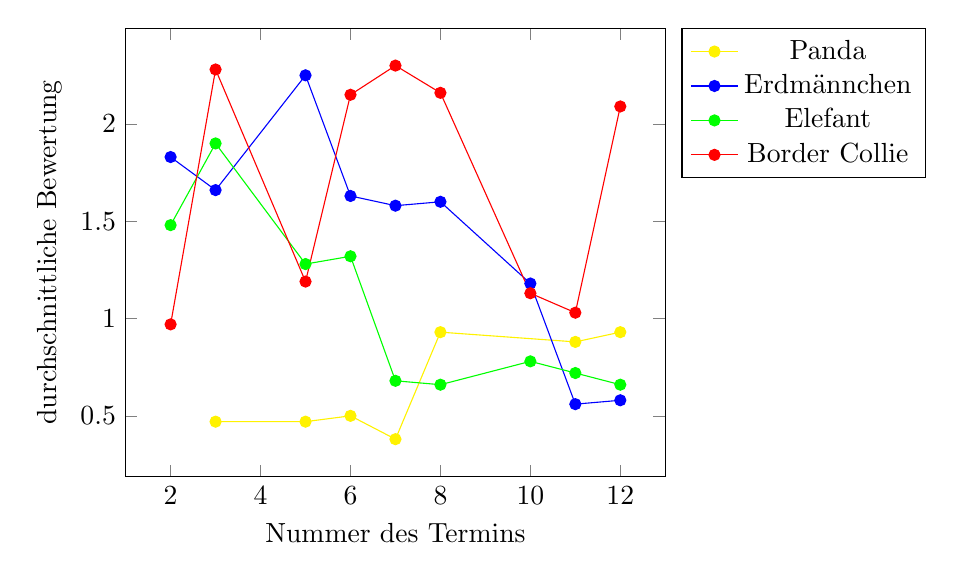
\begin{tikzpicture}
		\begin{axis}[legend pos=outer north east,xlabel={Nummer des Termins},ylabel={durchschnittliche Bewertung}]
			\addplot[mark=*,yellow]
			coordinates {
				(3,.47) (5,.47) (6,.5) (7,.38) (8,0.93) (11,.88) (12,.93)
			};
			\addlegendentry{Panda}
			\addplot[mark=*,blue]
			coordinates {
				(2,1.83)(3,1.66)(5,2.25)(6,1.63)(7,1.58)(8,1.6)(10,1.18)(11,.56)(12,.58)
			};
			\addlegendentry{Erdmännchen}
			\addplot[mark=*,green]
			coordinates {
				(2,1.48)(3,1.9)(5,1.28)(6,1.32)(7,0.68)(8,0.66)(10,.78)(11,.72)(12,.66)
			};
			\addlegendentry{Elefant}
			\addplot[mark=*,red]
			coordinates {
				(2,.97)(3,2.28)(5,1.19)(6,2.15)(7,2.3)(8,2.16)(10,1.13)(11,1.03)(12,2.09)
			};
			\addlegendentry{Border Collie}
			
		\end{axis}
	\end{tikzpicture}
	\caption{Entwicklung der kreativen Haltung}
\end{figure}	
	
	
\subsection{Konvergentes Denken}
\begin{figure}[H]
	\centering
	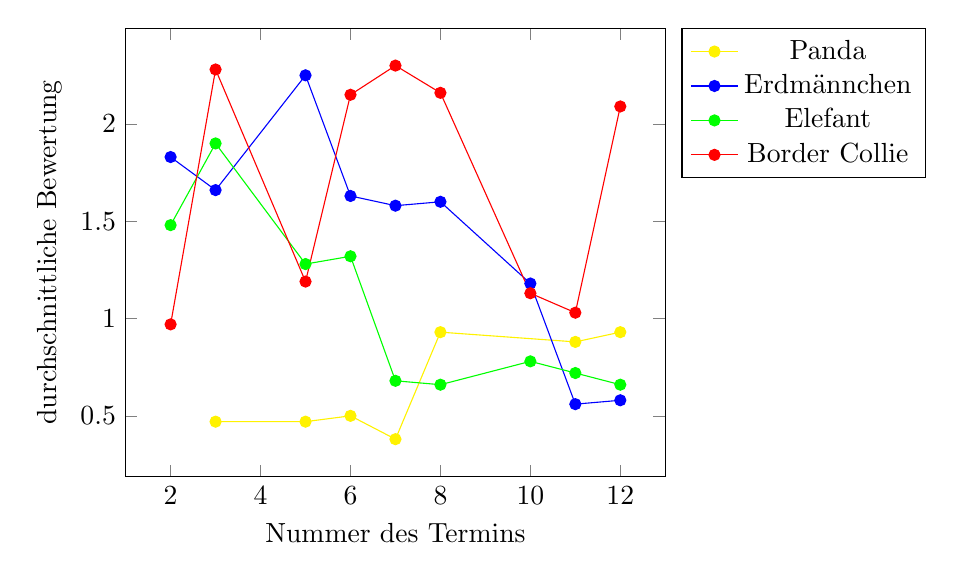
\begin{tikzpicture}
		\begin{axis}[legend pos=outer north east,xlabel={Nummer des Termins},ylabel={durchschnittliche Bewertung}]
			\addplot[mark=*,yellow]
			coordinates {
				(3,.47) (5,.47) (6,.5) (7,.38) (8,0.93) (11,.88) (12,.93)
			};
			\addlegendentry{Panda}
			\addplot[mark=*,blue]
			coordinates {
				(2,1.83)(3,1.66)(5,2.25)(6,1.63)(7,1.58)(8,1.6)(10,1.18)(11,.56)(12,.58)
			};
			\addlegendentry{Erdmännchen}
			\addplot[mark=*,green]
			coordinates {
				(2,1.48)(3,1.9)(5,1.28)(6,1.32)(7,0.68)(8,0.66)(10,.78)(11,.72)(12,.66)
			};
			\addlegendentry{Elefant}
			\addplot[mark=*,red]
			coordinates {
				(2,.97)(3,2.28)(5,1.19)(6,2.15)(7,2.3)(8,2.16)(10,1.13)(11,1.03)(12,2.09)
			};
			\addlegendentry{Border Collie}
			
		\end{axis}
	\end{tikzpicture}
	\caption{Entwicklung des konvergenten Denkens}
\end{figure}	

\section{Herkunft und Entwicklung}
Da wie bereits erwähnt die Daten der Parallelveranstaltung in Ägypten keine Vergleichsdaten zu den Persönlichkeitstests und den Computational Thinking Tests liefern, ist nur ein kultureller Vergleich beider Gruppen möglich. Deshalb werden im folgenden Abschnitt die beiden Studien in den fünf Bereichen miteinander verglichen.
\subsection{Teamwork}
\begin{figure}[H]
	\centering
	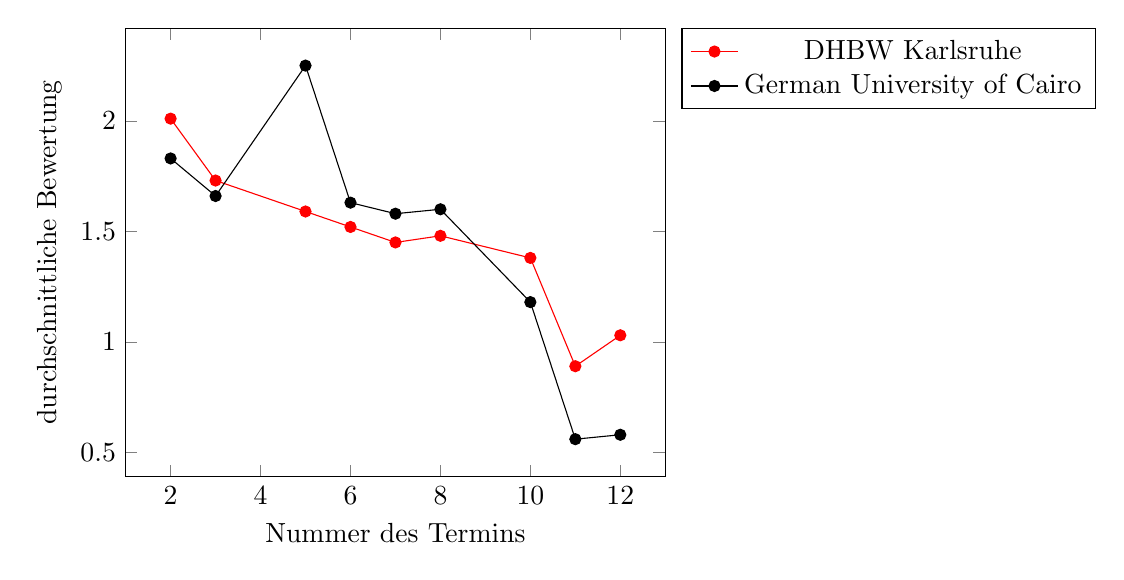
\begin{tikzpicture}
		\begin{axis}[legend pos=outer north east,xlabel={Nummer des Termins},ylabel={durchschnittliche Bewertung}]
			\addplot[mark=*,red]%Germany
			coordinates{
				(2,2.01)(3,1.73)(5,1.59)(6,1.52)(7,1.45)(8,1.48)(10,1.38)(11,0.89)(12,1.03)
			};
			\addlegendentry{DHBW Karlsruhe}
			\addplot[mark=*,black]
			coordinates {
				(2,1.83)(3,1.66)(5,2.25)(6,1.63)(7,1.58)(8,1.6)(10,1.18)(11,.56)(12,.58)
			};
			\addlegendentry{German University of Cairo}
			
		\end{axis}
	\end{tikzpicture}
	\caption{Entwicklung des konvergenten Denkens}
\end{figure}
\subsection{Divergentes Denken}
\begin{figure}[H]
	\centering
	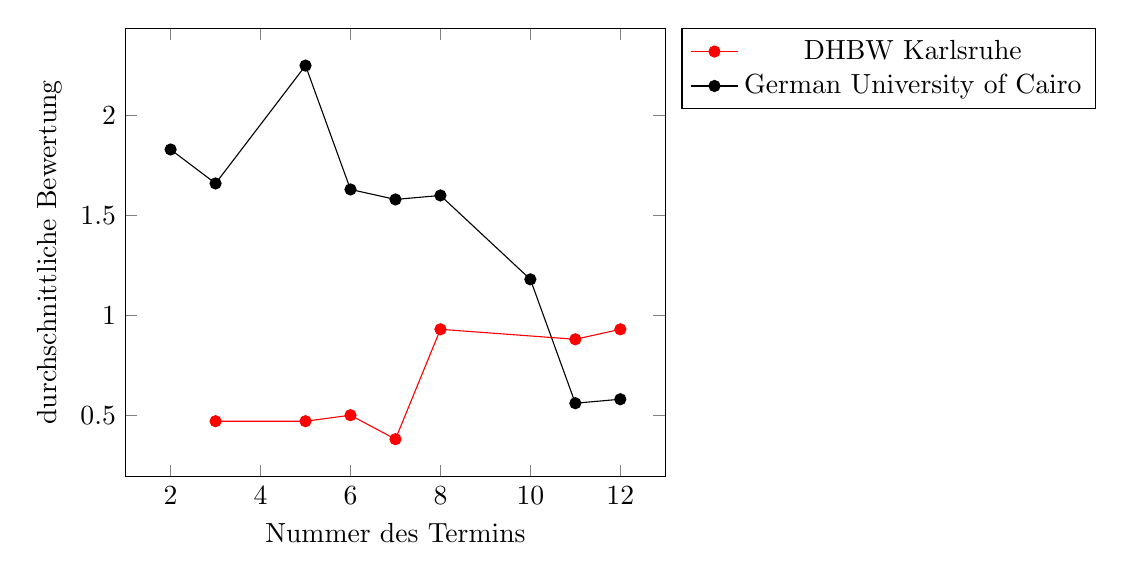
\begin{tikzpicture}
		\begin{axis}[legend pos=outer north east,xlabel={Nummer des Termins},ylabel={durchschnittliche Bewertung}]
			\addplot[mark=*,red]%Germany
			coordinates {
				(3,.47) (5,.47) (6,.5) (7,.38) (8,0.93) (11,.88) (12,.93)
			};
			\addlegendentry{DHBW Karlsruhe}
			\addplot[mark=*,black]
			coordinates {
				(2,1.83)(3,1.66)(5,2.25)(6,1.63)(7,1.58)(8,1.6)(10,1.18)(11,.56)(12,.58)
			};
			\addlegendentry{German University of Cairo}
			
		\end{axis}
	\end{tikzpicture}
	\caption[Vergleich Entwicklung Teamfähigkeit beider Veranstaltungen]{Vergleich der Entwicklung der Teamfähigkeit beider Veranstaltungen}
\end{figure}
\subsection{Emergentes Denken}
\begin{figure}[H]
	\centering
	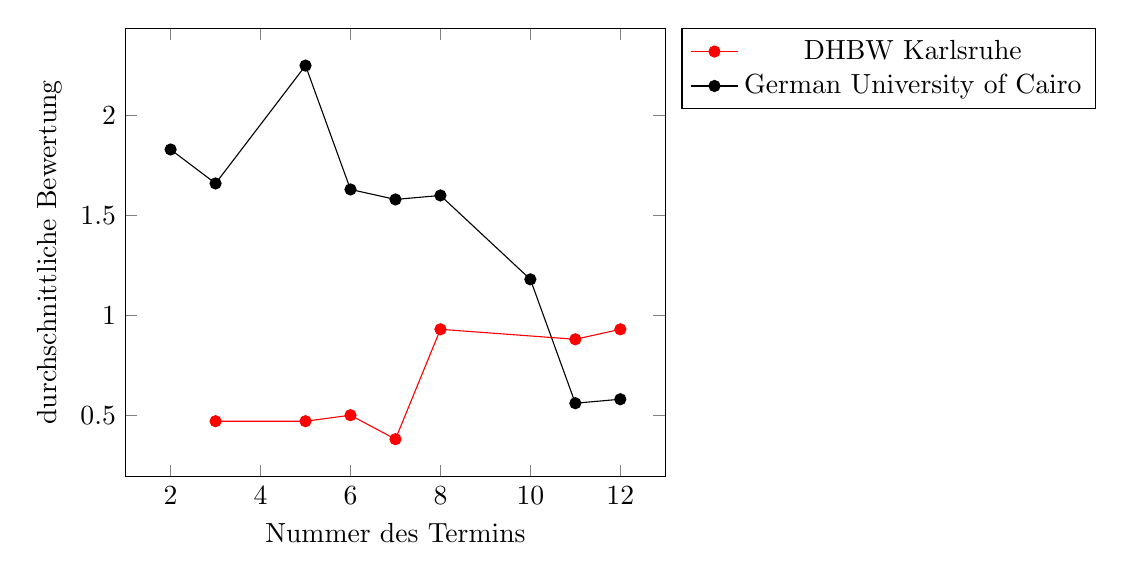
\begin{tikzpicture}
		\begin{axis}[legend pos=outer north east,xlabel={Nummer des Termins},ylabel={durchschnittliche Bewertung}]
			\addplot[mark=*,red]%Germany
			coordinates {
				(3,.47) (5,.47) (6,.5) (7,.38) (8,0.93) (11,.88) (12,.93)
			};
			\addlegendentry{DHBW Karlsruhe}
			\addplot[mark=*,black]
			coordinates {
				(2,1.83)(3,1.66)(5,2.25)(6,1.63)(7,1.58)(8,1.6)(10,1.18)(11,.56)(12,.58)
			};
			\addlegendentry{German University of Cairo}
			
		\end{axis}
	\end{tikzpicture}
	\caption[Vergleich Entwicklung emergentes Denken beider Veranstaltungen]{Vergleich der Entwicklung des emergenten Denkens beider Veranstaltungen}
\end{figure}
\subsection{Kreative Haltung}
\begin{figure}[H]
	\centering
	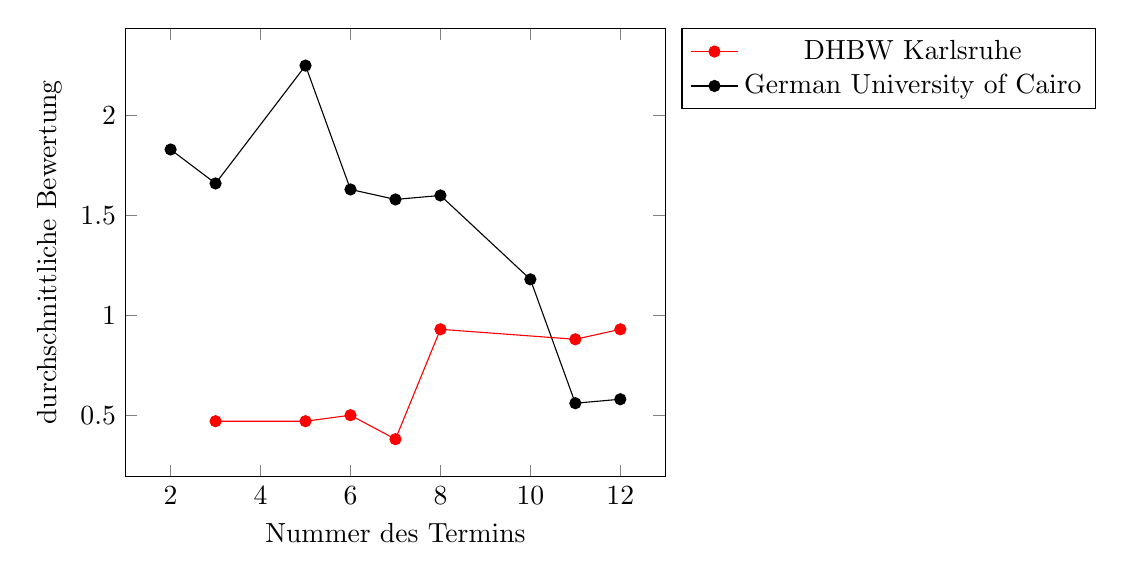
\begin{tikzpicture}
		\begin{axis}[legend pos=outer north east,xlabel={Nummer des Termins},ylabel={durchschnittliche Bewertung}]
			\addplot[mark=*,red]%Germany
			coordinates {
				(3,.47) (5,.47) (6,.5) (7,.38) (8,0.93) (11,.88) (12,.93)
			};
			\addlegendentry{DHBW Karlsruhe}
			\addplot[mark=*,black]
			coordinates {
				(2,1.83)(3,1.66)(5,2.25)(6,1.63)(7,1.58)(8,1.6)(10,1.18)(11,.56)(12,.58)
			};
			\addlegendentry{German University of Cairo}
			
		\end{axis}
	\end{tikzpicture}
	\caption[Vergleich Entwicklung kreative Haltung beider Veranstaltungen]{Vergleich der Entwicklung der kreativen Haltung beider Veranstaltungen}
\end{figure}
\subsection{Konvergentes Denken}
\begin{figure}[H]
	\centering
	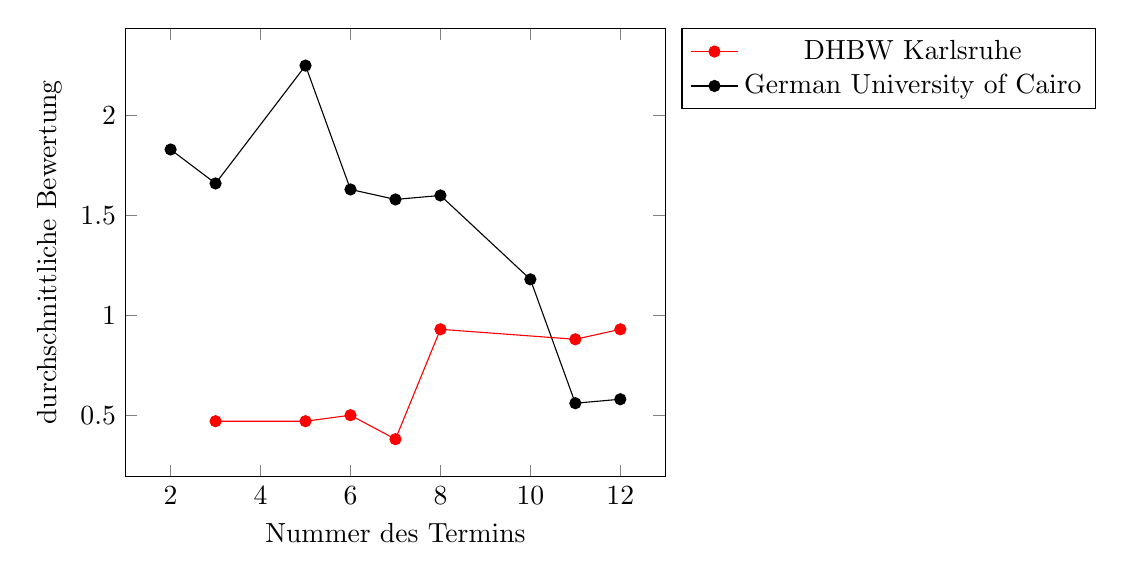
\begin{tikzpicture}
		\begin{axis}[legend pos=outer north east,xlabel={Nummer des Termins},ylabel={durchschnittliche Bewertung}]
			\addplot[mark=*,red]%Germany
			coordinates {
				(3,.47) (5,.47) (6,.5) (7,.38) (8,0.93) (11,.88) (12,.93)
			};
			\addlegendentry{DHBW Karlsruhe}
			\addplot[mark=*,black]
			coordinates {
				(2,1.83)(3,1.66)(5,2.25)(6,1.63)(7,1.58)(8,1.6)(10,1.18)(11,.56)(12,.58)
			};
			\addlegendentry{German University of Cairo}
			
		\end{axis}
	\end{tikzpicture}
	\caption[Vergleich Entwicklung konvergentes Denken beider Veranstaltungen]{Vergleich der Entwicklung des konvergenten Denkens beider Veranstaltungen}
\end{figure}

\section{Computational Thinking Test}
	In dem folgenden Abschnitt wird die Auswertung der Ergebnisse des \acrshort{bctt}, welcher zu Beginn der Studie durchgeführt wurde, sowie die des \acrshort{cctt}, welcher nach Abschluss aller Termine von den Kindern bearbeitet wurde. Die Ergebnisse der beiden Tests befinden sich im Kapitel \ref{sec:ErgebnisseCTT}.
	\subsection{BCTt}
	In Kapitel \ref{sec:ct} wurde aufgeführt, welche Ergebnisse bei einer Durchführung des \acrshort{bctt} bei einer Stichprobe von 299 Schülern und Schülerinnen auftreten. Anhand dieser Daten kann nun die Gruppe der Kinder, die an dieser Studie an der \acrshort{dhbw} Karlsruhe teilnahmen, in ihrem informatischen Denken eingeordnet werden. Dazu werden die Daten der Kinder aus Tabelle \ref{tab:data} in der untenstehenden Tabelle noch einmal aufbereitet, so dass ein guter Vergleich gezogen werden kann. Generell ist zu beachten, dass die Stichprobe, die von \citeauthor{bcct} aufgeführt wurde, eine deutlich höhere Anzahl an Teilnehmern hat als die Anzahl, die in dieser Studienarbeit zur Verfügung stand. Dadurch kann nur beurteilt werden, ob die Kinder dieser Studie dem Durchschnitt entsprachen oder über- bzw. unterdurchschnittlich abschnitten.
	\begin{table}[H]
		\centering
		\begin{tabular}{|l|l|l|l|}
			\hline
			\rowcolor[HTML]{C0C0C0} 
			\textbf{Klassenstufe} & \textbf{Anzahl} & \textbf{Durchschnitt} & \textbf{Std. Abweichung} \\ \hline
			2                     & 6               & 19.5                  & 5,188                    \\ \hline
			3                     & 2               & 24                    & 1                        \\ \hline
		\end{tabular}
	\label{tab:statisticAufbereitung}
	\caption{Statistische Aufbereitung der Werte der Tabelle \ref{tab:data}}
	\end{table}

	Für die Altersgruppe der Kinder, die sich während des Tests in der dritten Klassenstufe befanden, existieren seitens der Autoren des \acrshort{bctt} keine Vergleichsdaten. Die Kinder, die die dritte Stufe besuchten, übertrafen im Vergleich zu den Daten aus Tabelle \ref{tab:statisticsBCTT}. Diese Kinder schnitten im Durchschnitt besser ab und die Standardabweichung lag auch deutlich unter den von \citeauthor{bcct} angegebenen Daten. Die Stichprobe, die von den Autoren dieser Studienarbeit durchgeführt wurde, ist jedoch nicht sehr groß, weshalb die Aussagekraft über das Abschneiden der Kinder nicht sehr hoch ist.\\
	Anders sieht es bei den Kindern der Klassenstufe Zwei aus. Wie aus der obenstehenden Tabelle zu entnehmen ist, lag der Durchschnitt, den die Kinder beim Bearbeiten des \acrlong{bctt} erzielten, zwar ebenfalls über dem Durchschnitt aus Tabelle \ref{tab:statisticsBCTT}, jedoch ist die Standardabweichung, die für diese Gruppe ermittelt wurde, doppelt so hoch als die Vergleichsdaten der Kinder aus Spanien. Wie aus der Tabelle \ref{tab:data} erkennbar ist, lag die Streuung der Ergebnisse der Kinder, die die Klassenstufe Zwei besuchten, in einem Bereich von 10 Punkten bis hin zur maximal erreichbaren Punktzahl von 25 Punkten.   
	\subsection{CCTt}
	Der \acrshort{cctt} fiel im Vergleich zum \acrshort{bctt} wie erwartet schlechter aus. Wenig überraschend dagegen ist das Abschneiden der Elefanten und auch das der Erdmännchen, da diese bereits im \acrshort{bctt} sehr gut abgeschnitten hatten. Ein großes Problem der Kinder war die Zeit. Das wird anhand der Punkte, die die Kinder in den einzelnen Kategorien erreicht haben, ersichtlich, da Kategorien, die weiter hinten angesiedelt waren, aufgrund der Zeit nicht bearbeitet wurden. Auffallend sind daher die Ergebnisse des Persönlichkeitstyps Panda, da dieser im \acrshort{bctt} schlechter abgeschnitten hatte. Da alle anderen Gruppen in den Typen weiter rechts auf der X-Achse weniger Punkte sammelten und auch bei Sara kein zufälliges bzw. unsortiertes Lösen der Aufgaben beobachtet werden konnte, gibt es hierfür einen anderen Grund. Beim Korrigieren des \acrshort{cctt} ist aufgefallen, dass weiter hinten Sara vermutlich aus Zeitgründen immer die gleiche Antwort angekreuzt hat. Dadurch hatte sie viel Glück und die Antworten waren sogar teilweise richtig, jedoch verfälschte das das Ergebnis. Also wurde um Glücksantworten zu filtern für falsche Fragen ein Minuspunkt berechnet, für nicht beantwortete Fragen kein Punkt. So kann überprüft werden, ob die Kinder wirklich die Antworten wussten oder eben Glückstreffer dabei waren. Dabei ergab sich nach Abzug der falschen Punkte die untenstehenden Werte.
	
	
	\pgfplotstableread[row sep=\\,col sep=&]{
		Name &Ohne Abzug &Mit Abzug \\
		Henriette     & 4  & 1 \\
		Moritz     & 16 & 15 \\
		Heinz    & 0 & 0\\
		Benny   & 11 & 11\\
		Lulu   & 6  & 4\\
		Mario      & 3 & -5\\
		Sara &6 & -6\\
		Jonas&3 & -2\\
	}\mydata

	\begin{figure}[H]
		\begin{tikzpicture}
			\begin{axis}[ ybar,
				bar width=.5cm,
				width=\textwidth,
				height=.5\textwidth,
				legend style={at={(0.5,1)},
					anchor=north,legend columns=-1},
				symbolic x coords={Henriette, Moritz, Heinz, Benny, Lulu, Mario, Sara, Jonas},
				xtick=data,
				nodes near coords,
				nodes near coords align={vertical},
				ymin=-10,ymax=20,
				ylabel={Anzahl erreichter Punkte}, xlabel = {Name des Kindes}]
				\addplot table[x=Name,y=Ohne Abzug]{\mydata};
				\addplot table[x=Name,y=Mit Abzug]{\mydata};
				\addlegendentry{Ohne Abzug}
				\addlegendentry{Mit Abzug}
			\end{axis}
		\end{tikzpicture}
		\caption[Änderungen Punktzahlen nach Abzug]{Änderungen der Punktzahlen nach Abzug der falschen Antworten}
		\label{img:wrongAnswerCorrection}
	\end{figure}

	Auffallend ist, wie bereits vermutet, das Ergebnis von Sara. Statt voher insgesamt sechs korrekt beantworteten Fragen hatte sie nun ein Ergebnis von -6, also zwölf falsch beantwortete Fragen. Natürlich kann hier angemerkt werden, dass die Kinder nicht wussten, dass wir für falsche Fragen Punkte abziehen, ihre Anweisungen waren lediglich: \glqq Es ist nicht wichtig, dass du alle Fragen beantwortest\grqq. Deshalb könnte dies anders ausfallen, sollten die Kinder vorher darüber informiert werden. Bei dem Großteil der Kinder zeigte sich jedoch, dass die Fragen, die sie beantwortet hatten, korrekt waren und Fragen, die sie nicht beantworten konnten, übersprungen wurden. Die Abzüge waren meist nur sehr gering. Lediglich die 12-Punkte-Differenz bei Sara zeigt, dass die Ergebnisse aus \ref{img:auswertung_typus_ctt} verfälscht sind und man daraus nicht schließen kann, dass sie in diesen Bereichen besser ist als die anderen Kinder.\\
	Ebenso ist auch das Ergebnis von Mario. Auch er verlor einen Großteil seiner Punkte durch den Abzug falscher Antworten. Er hatte den Test nach nicht einmal sieben Minuten beendet und einige Aufgaben übersprungen, bei denen er keine Antwort wusste. Statt die 13 Minuten, die er noch hatte, zu nutzen und seine Antworten zu überprüfen, gab er ab und schnitt dementsprechend schlecht ab. Hier spielte also weniger die Zeit eine Rolle, als das Wissen bzw. die Fähigkeit, das Computational Thinking anzuwenden.\\
	Aufgrund der nicht zufälligen Bearbeitung kann für weiter hinten angesiedelte Typen auch kein Vergleich zwischen den einzelnen Typen gezogen werden, lediglich kann bewertet werden, wie gut die Kinder in den ersten drei Kategorien abschnitten. Über den zeitlichen Verlauf kann gesagt werden, dass Kinder, die in den hinteren Aufgaben mehr Punkte holten, in den vorderen Kategorien besser sind als Kinder, die weiter hinten weniger Punkte holten, da sich daraus schließen lässt, dass die besseren Kinder weniger Zeit bei den ersten Aufgaben in Anspruch nehmen mussten. Dies würde bedeuten, dass die Kinder der beiden Typen Elefant und Erdmännchen in den vorderen Kategorien besser waren, im direkten Vergleich sind die Elefanten jedoch besser, da diese im Durchschnitt mehr Punkte erzielten. Innerhalb der beiden Typen gibt es jedoch große Diskrepanzen zwischen den einzelnen Kindern, beispielsweise erzielte Moritz in fast allen Kategorien Punkte, während Lulu nur in den ersten beiden Kategorien Punkte sammeln konnte. Dasselbe ist auch zwischen Benny und Henriette sichtbar, auch hier zeigen sich Differenzen zwischen den beiden Kindern in den gesammelten Punkten.\\
	Wie auch bei den Entwicklungen schneiden die beiden Typen auch aufgrund der Altersunterschiede der Kinder deutlich besser ab, da diese in ihrer geistigen Entwicklung aufgrund des Alters fortgeschrittener sind und somit mit diesen schwereren Fragen besser klar kommen. Der \acrshort{cctt} ist zudem genau für diese Altersgruppe ausgelegt, in der sich Benny und Moritz befinden, weshalb sie hier einen Vorteil im Vergleich zu den anderen Kindern haben.
    \chapter{Diskussion}

\section{Fazit}



\section{Verbesserungen}
\subsection{Gruppengröße}
Die aus der Beobachtung der Kinder gewonnenen Daten 




\begin{itemize}
	\item gleiche Testbedingungen
	\item größere Gruppen
	\item andere Gruppenkonstellationen
	\item verbesserte Skalierung bei der Bewertung des CT
\end{itemize}


\end{onehalfspace}

\clearpage
\pagenumbering{roman}
\setcounter{page}{4}
\appendix

% bibliography
\printbibliography[title={Literaturverzeichnis}]
\addcontentsline{toc}{chapter}{Literaturverzeichnis}

\printglossary

\chapter{Beobachtungsbogen}

\begin{figure}[h]
	\centering
	\begin{tabular}{@{}c@{\hspace{.5cm}}c@{}}
		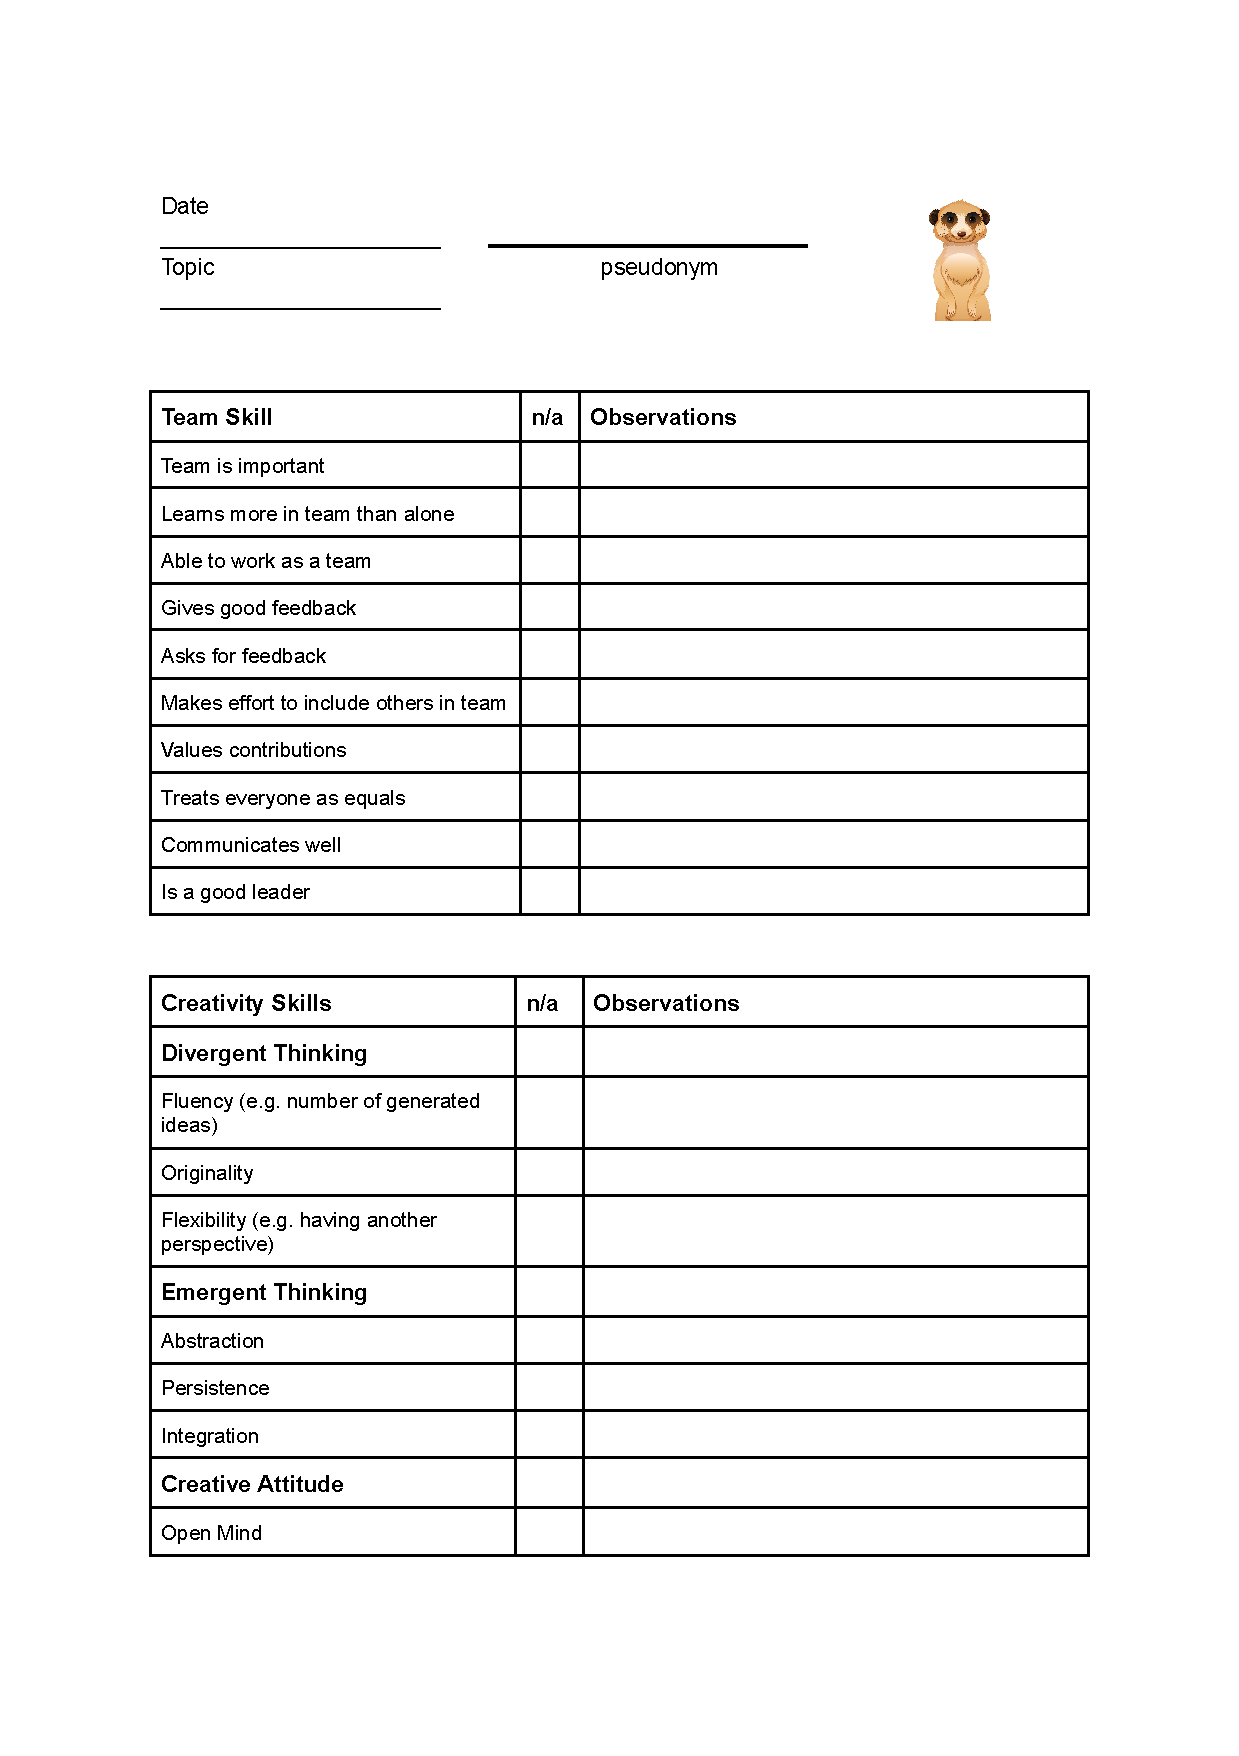
\includegraphics[page=1,width=.45\textwidth]{observation_sheets} & 
		\includegraphics[page=2,width=.45\textwidth]{observation_sheets} \\
	\end{tabular}
	\caption{Beobachtungsbogen Beispiel}
	\label{pdf:observation_sheets}
\end{figure}




\end{document}
